\graphicspath{{Figures/}}

\title{\fontsize{33}{45}{\huge Pattern Classification (EET 3035)\newline \vspace{8pt} \Large Lecture 02\vspace{-1.1cm}}}
\author{\vspace{-0.4cm}\\\normalsize{\bf Dr. Kundan Kumar}\\ PhD (IIT Kharagpur)\\
Associate Professor\\Department of ECE}
% - Give the names in the same order as the appear in the paper.
% - Use the \inst{?} command only if the authors have different
%   affiliation.

\institute[Indian Institute of Technology Kharagpur] % (optional, but mostly needed)
{

\includegraphics[height=.17\textheight]{SOAlogo.png}\\
 Faculty of Engineering (ITER)\\ S`O'A Deemed to be University, Bhubaneswar, India-751030\\
 \copyright\  2020 Kundan Kumar, All Rights Reserved\\
  \vspace{-1.1cm}}
% - Use the \inst command only if there are several affiliations.
% - Keep it simple, no one is interested in your street address.
\date{}
% To remove page number from a perticular slide
{
\setbeamertemplate{logo}{}
\makeatletter
\setbeamertemplate{footline}{
        \leavevmode%
  
  % First line.
  \hbox{%
  \begin{beamercolorbox}[wd=.2\paperwidth,ht=\beamer@decolines@lineup,dp=0pt]{}%
  \end{beamercolorbox}%
  \begin{beamercolorbox}[wd=.8\paperwidth,ht=\beamer@decolines@lineup,dp=0pt]{lineup}%
  \end{beamercolorbox}%
  } %
  % Second line.
  \hbox{%
  \begin{beamercolorbox}[wd=\paperwidth,ht=\beamer@decolines@linemid,dp=0pt]{linemid}%
  \end{beamercolorbox}%
  } %
  % Third line.
  \hbox{%
  \begin{beamercolorbox}[wd=.1\paperwidth,ht=\beamer@decolines@linebottom,dp=0pt]{}%
  \end{beamercolorbox}%
  \begin{beamercolorbox}[wd=.9\paperwidth,ht=\beamer@decolines@linebottom,dp=0pt]{linebottom}%
  \end{beamercolorbox}%
  }%
        }
\makeatother
\begin{frame}
\titlepage
\end{frame}
}

\section{Feature Extraction}
\subsection{}
\begin{frame}{}
\begin{variableblock}{\centering \Large \textbf{\vspace{4pt}\newline Feature Extraction\vspace{4pt}}}{bg=slidecolor,fg=white}{bg=slidecolor,fg=white}
\end{variableblock}
\end{frame}

\begin{frame}{Topics to be covered}
\begin{itemize}
%\setlength{\itemsep}{-2pt}
\item Boundary Representation\nocite{gonzalez2002digital}
\begin{itemize}
\setlength{\itemsep}{-2pt}
\item Boundary (Border) following
\item Chain codes
\item Polynomial Approximation
\item Signatures
\item Boundary Segments
\item Skeletons
\end{itemize}
\item Boundary Descriptors
\begin{itemize}
\setlength{\itemsep}{-2pt}
\item Some Simple Descriptors
\item Shape Numbers
\item Fourier Descriptors
\item Statistical Moments
\end{itemize}
\item Regional Descriptors
\begin{itemize}
\setlength{\itemsep}{-2pt}
\item Texture: Moment Invariants
\item Texture: GLCM, LBP
\end{itemize}
\item Transformed domain features
\begin{itemize}
\item 2D-Gabor filter features
\end{itemize}
\end{itemize}
\end{frame}

\begin{frame}{Introduction to feature extraction}
\begin{itemize}
\item Scale invariant
\item Translation invariant
\item Rotation invariant
\item Luminance invariant
\end{itemize}
\vspace{-12pt}
\begin{figure}
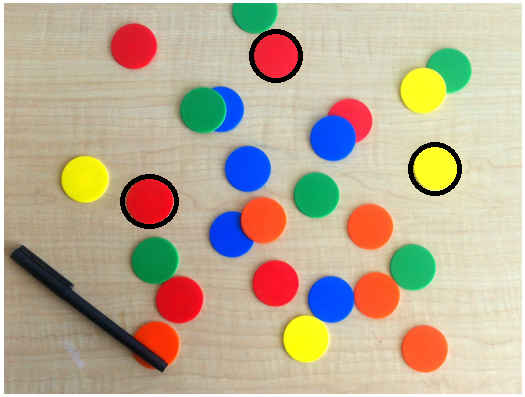
\includegraphics[height=4cm]{ArcCircle.png}~~~~
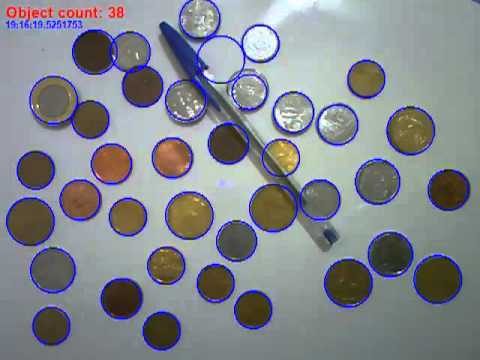
\includegraphics[height=4cm]{ArcCircle01.jpg}
\end{figure}
\end{frame}

\begin{frame}{Feature extraction from an ECG signal}
\begin{figure}
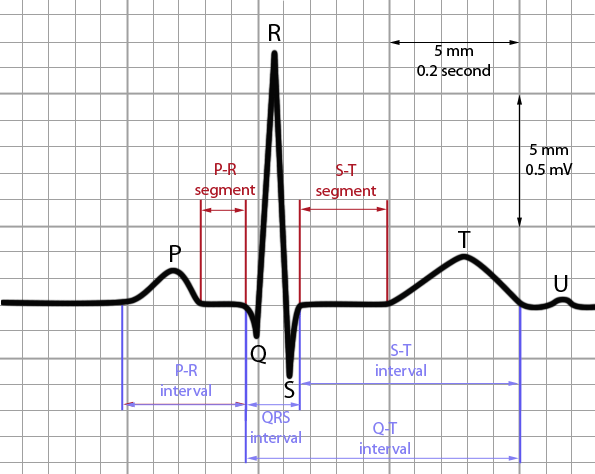
\includegraphics[height = 5cm]{ECG02.png}\\
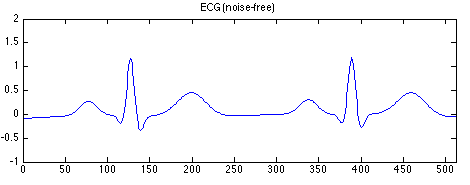
\includegraphics[width = 0.5\textwidth]{Figures/ECG01a.png}~~~
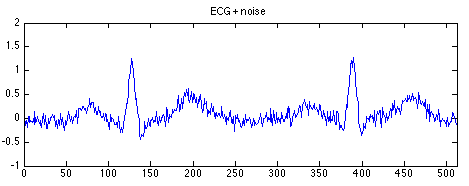
\includegraphics[width = 0.5\textwidth]{Figures/ECG01b.png}
\end{figure}
\end{frame}

\begin{frame}{Good features and Bad features}
\begin{itemize}
\item Extract features which are good for {\color{maroon}classification}.
\item {\color{maroon}Good features}:
\begin{itemize}
\item Objects from the same class have similar feature values
\item Objects from different classes have different values.
\end{itemize}
\item {\color{maroon}Bad Features:} features simply do not contain the information needed to separate the classes, doesn't matter how much effort you put into designing the classifier.
\end{itemize}
\begin{figure}
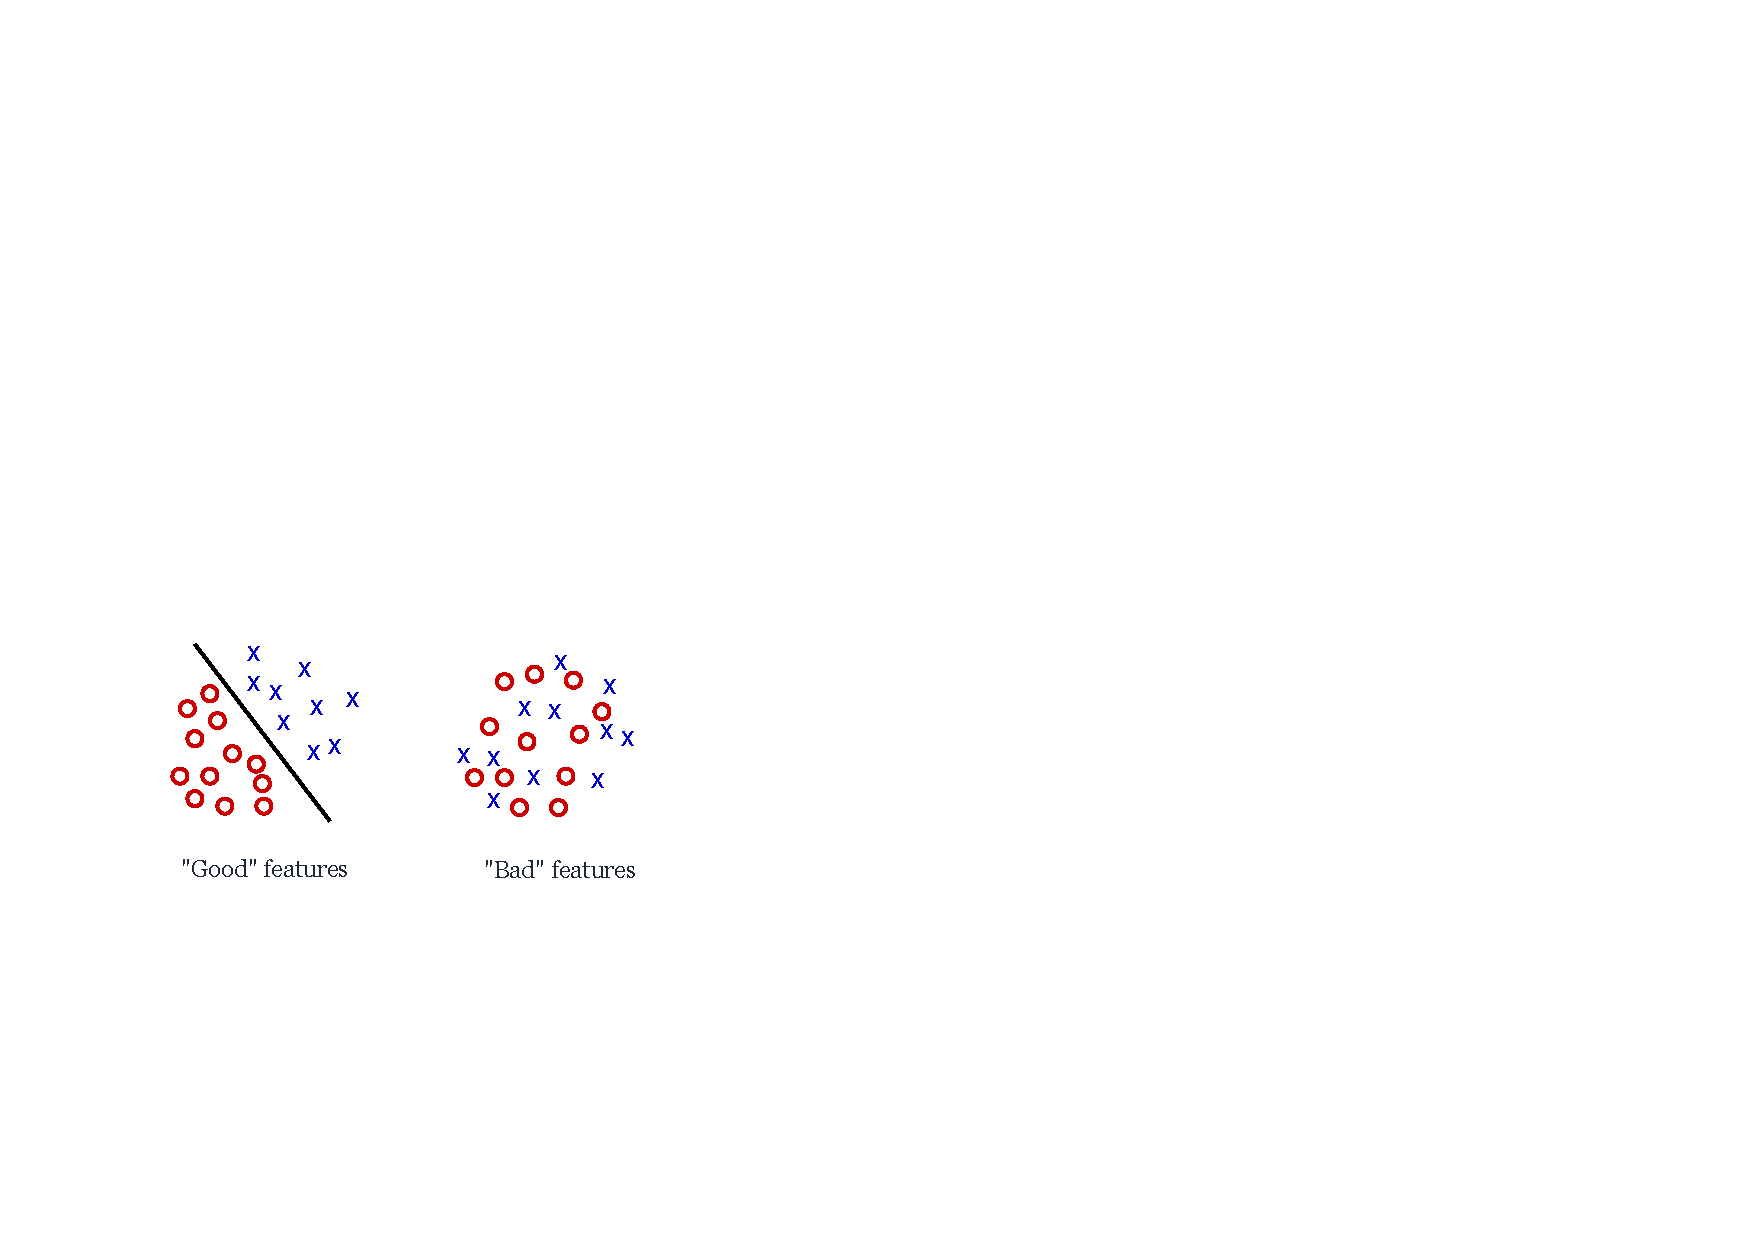
\includegraphics[scale=0.7]{Figures/goodbadFeatures}
\end{figure}
\end{frame}

\begin{frame}{Feature separability}
\begin{figure}
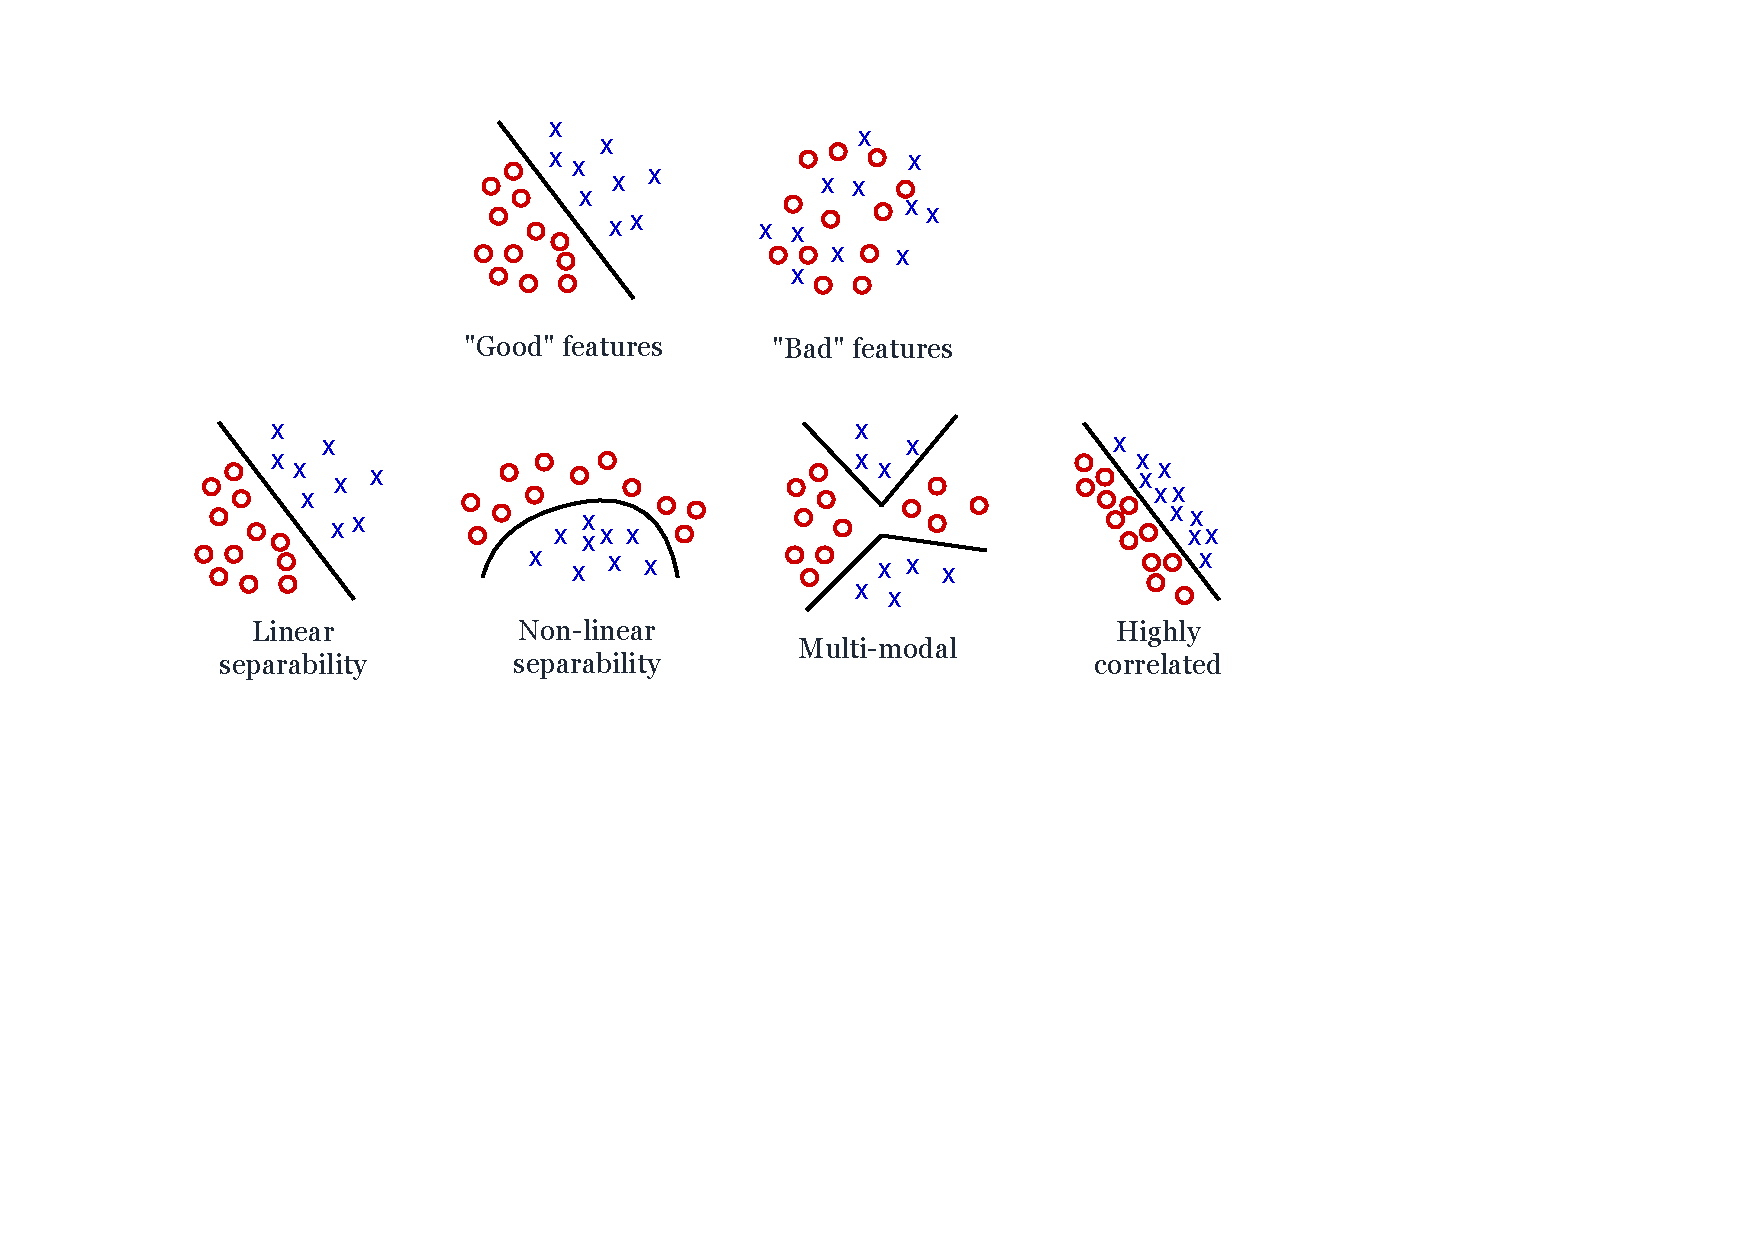
\includegraphics[scale=0.63]{Figures/FeatureSep}
\end{figure}
\end{frame}

\begin{frame}{Nature of separating plane?}
\begin{itemize}
\item For 2 dimensional feature space -- {\color{maroon}line}
\item For 3 dimensional feature space -- {\color{maroon}plane}
\item For more than 3 dimensional feature space -- {\color{maroon}hyperplane}
\end{itemize}
\begin{figure}
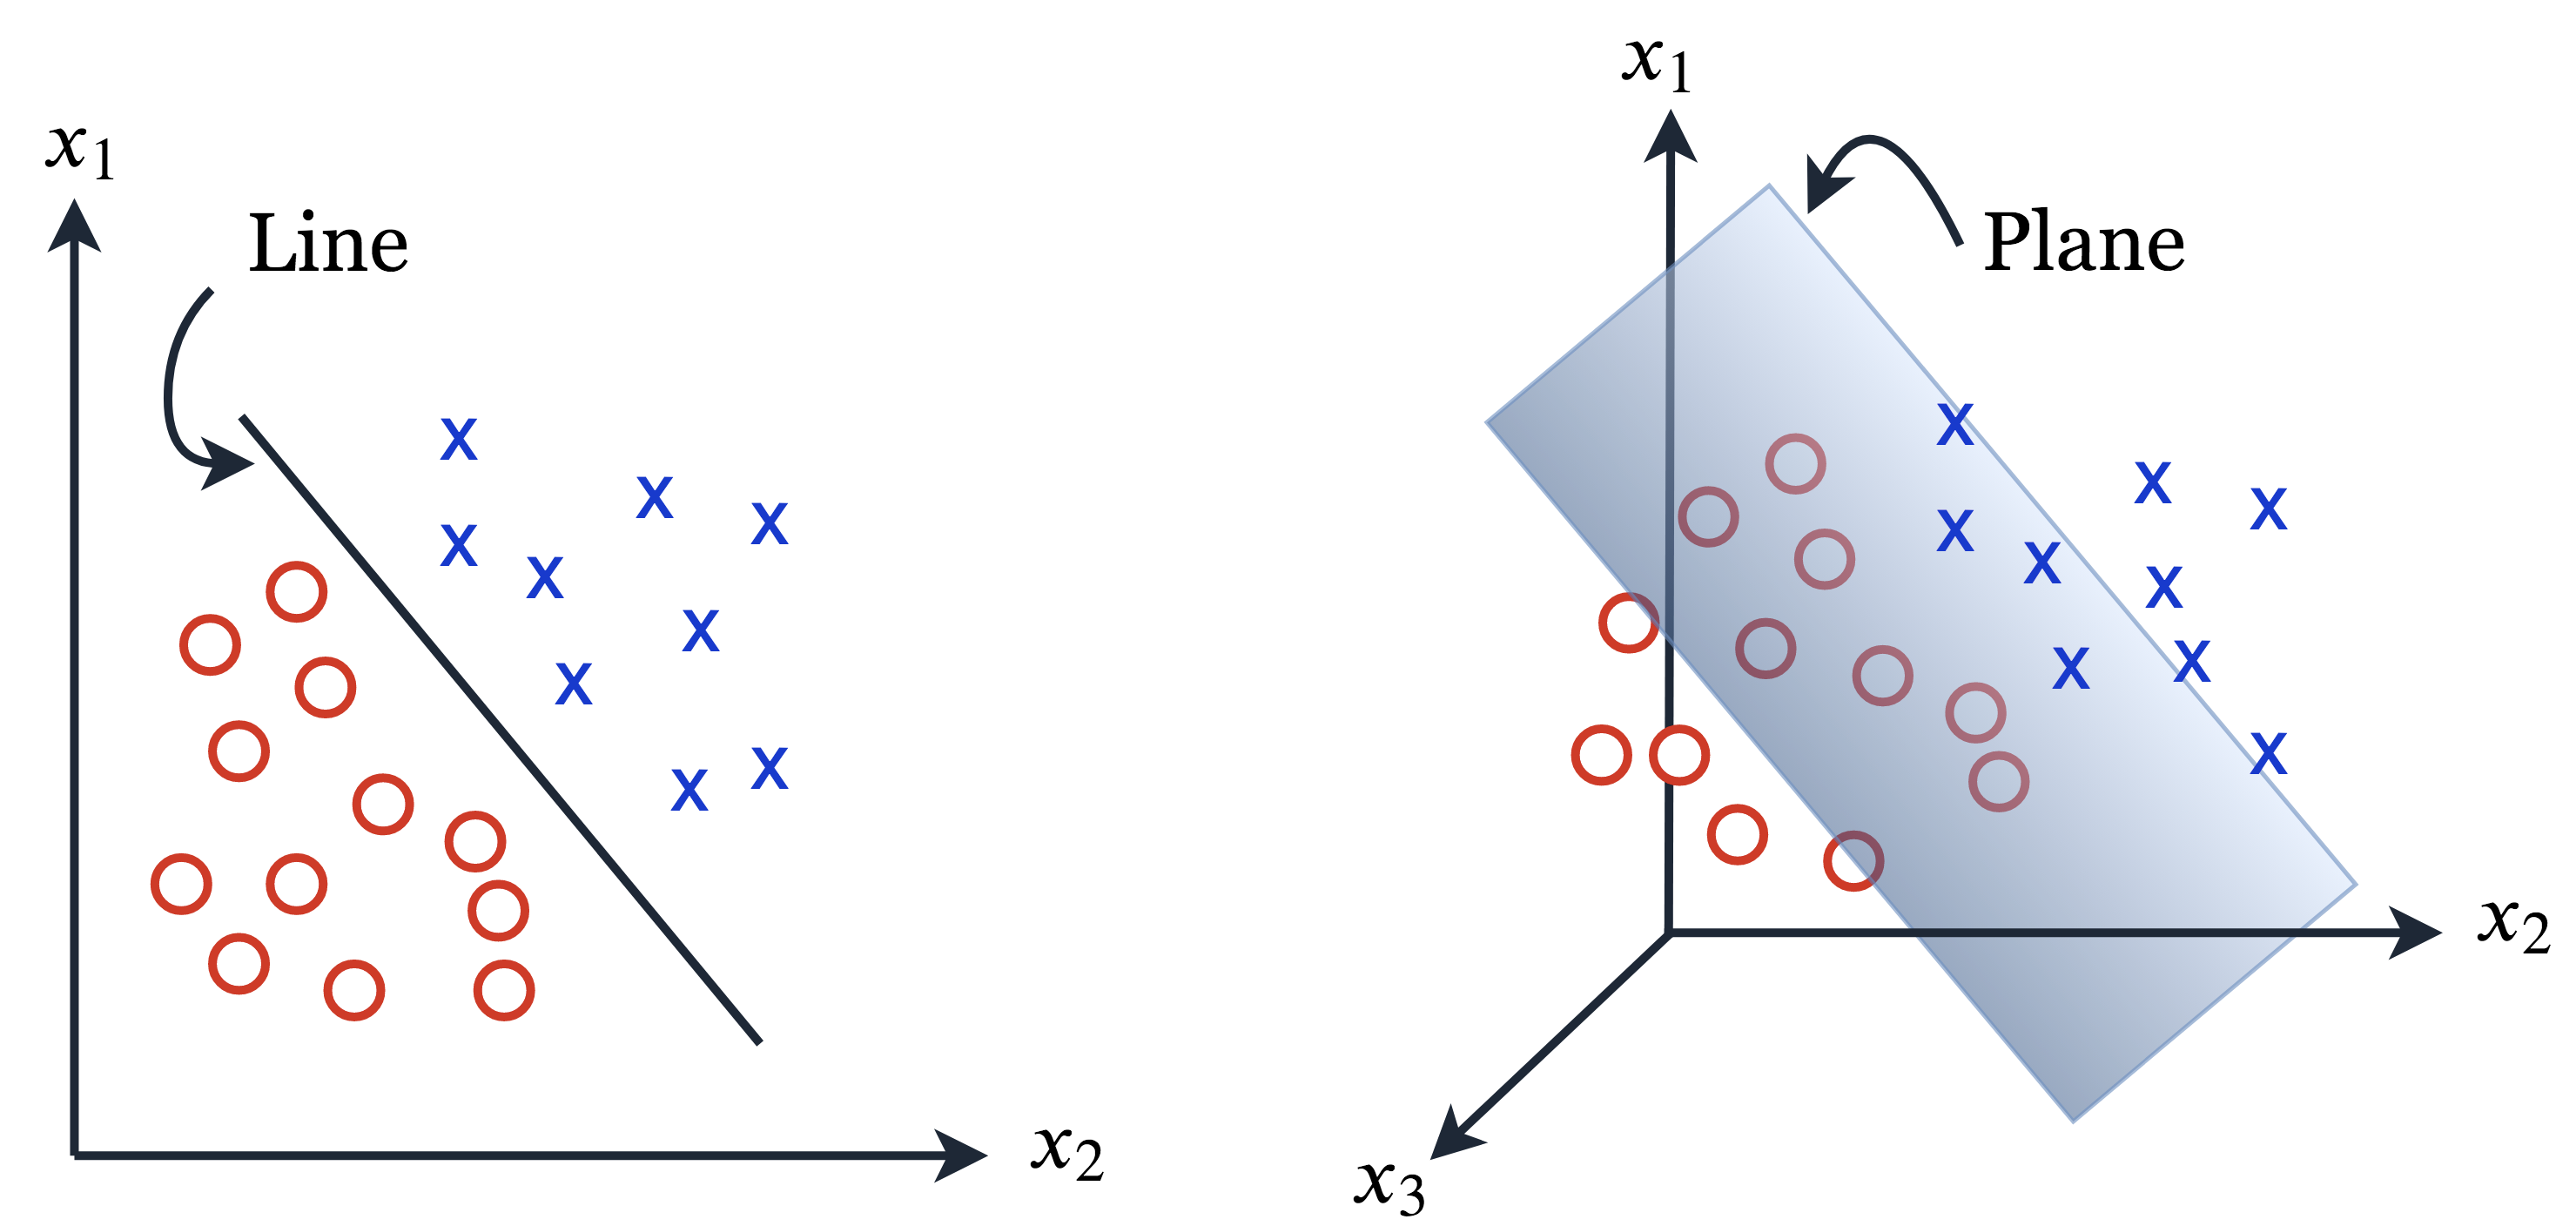
\includegraphics[scale=0.36]{Figures/Plane.png}
\end{figure}
\end{frame}

\begin{frame}{Labeled features}
\begin{columns}
\begin{column}{5cm}
\begin{figure}
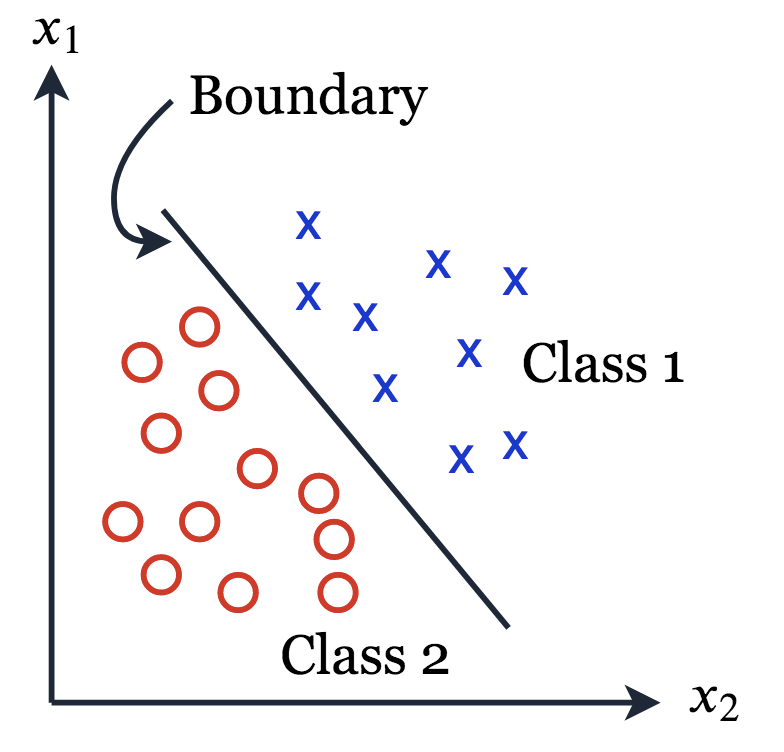
\includegraphics[scale=0.65]{Figures/label.png}
\end{figure}
\end{column}
\begin{column}{5cm}
\[\begin{array}{*{20}{c}}
{\left. {\begin{array}{*{20}{c}}
{{f_1}}\\
{{f_2}}\\
{{f_3}}
\end{array}} \right\} \in {C_1}}\\
{\left. {\begin{array}{*{20}{c}}
{{f_4}}\\
{{f_5}}\\
{{f_6}}\\
{{f_7}}
\end{array}} \right\} \in {C_2}}
\end{array}\]
\end{column}
\end{columns}
\begin{itemize}
\item In general, we use labeled features for supervised learning.
\end{itemize}
\end{frame}

\begin{frame}{Some property of features}
\begin{itemize}
\item The mapping from pattern to features that is unique whereas mapping from feature vector to pattern is not immediate.
\item So many patterns may be matched to the same feature of vector.
\item In pattern recognition, we never talk about a single pattern. We always talk about {\color{maroon}feature vector}.
\end{itemize}
\vspace{12pt}
\textbf{Types of Boundary Features:}
\begin{enumerate}
\item Boundary features/Descriptors
\item Region features/Descriptors
\end{enumerate}
\end{frame}

\section{Boundary Representation}
\subsection{}
\begin{frame}{}
\begin{variableblock}{\centering \Large \textbf{\vspace{4pt}\newline Boundary Representation\vspace{4pt}}}{bg=slidecolor,fg=white}{bg=slidecolor,fg=white}
\end{variableblock}
\begin{figure}
\centering
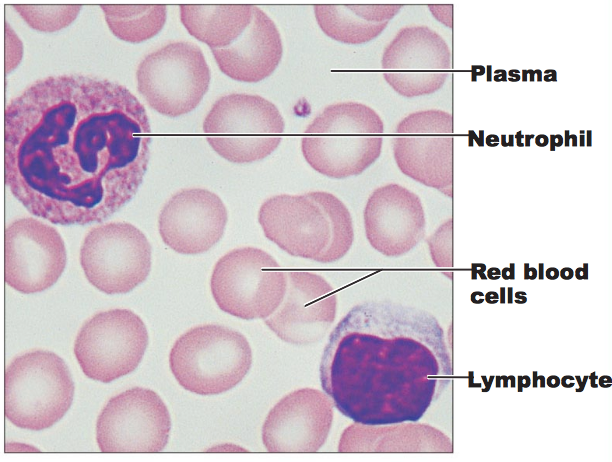
\includegraphics[width=4cm]{Figures/Paper0.png}\\\vspace{4pt}
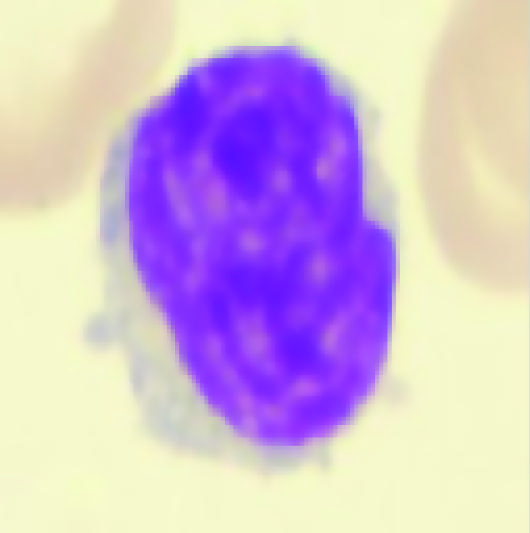
\includegraphics[width=2.5cm]{Figures/Paper1.jpg}~~~~~~
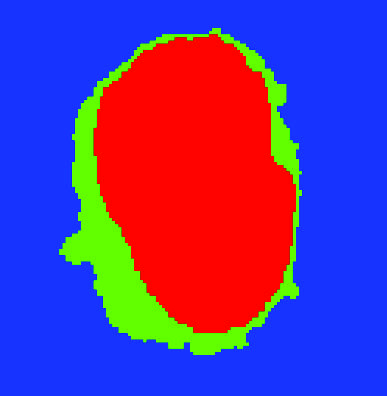
\includegraphics[width=2.5cm]{Figures/Paper2.jpg}~~~~~~
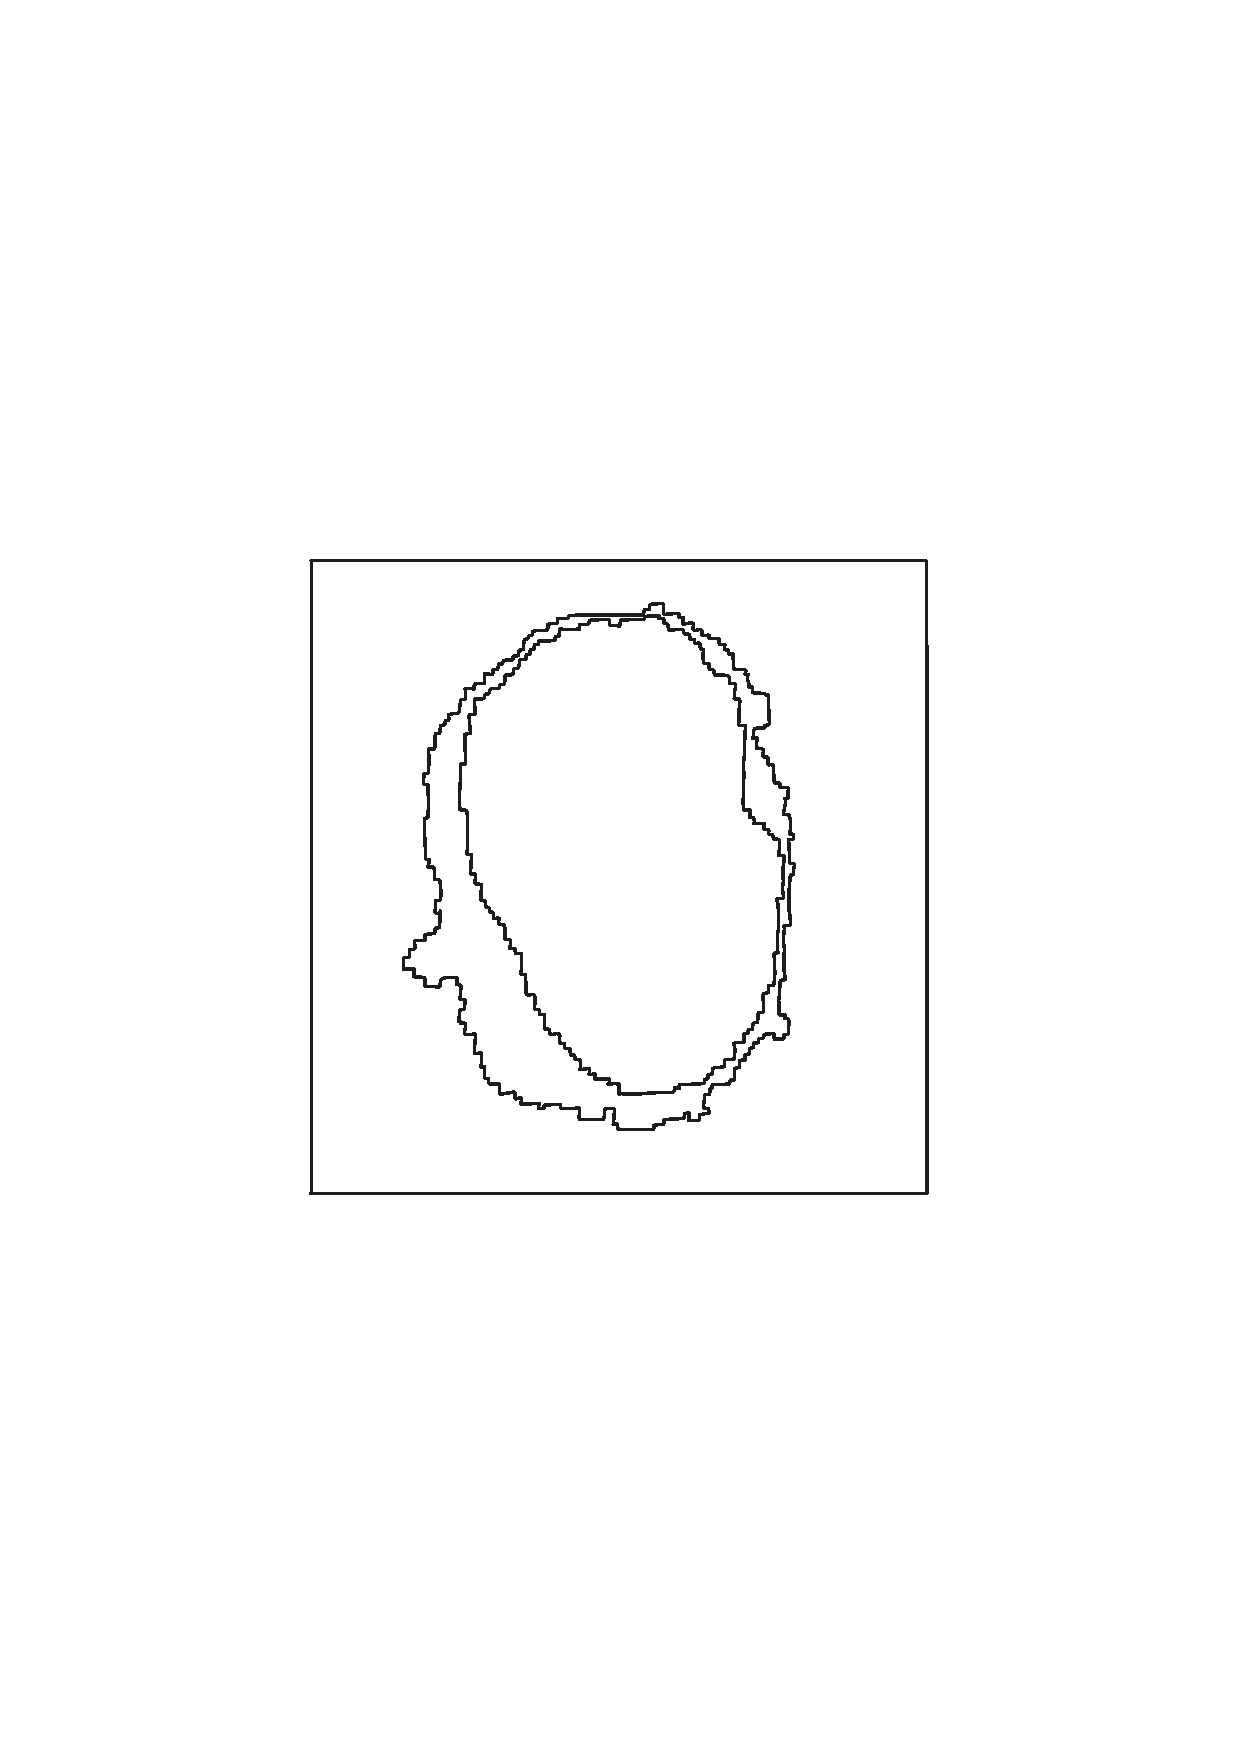
\includegraphics[width=2.5cm]{Figures/Paper3}
\end{figure}
\end{frame}

\begin{frame}{Binary Images}
\begin{figure}

\includegraphics[scale=0.35]{Binary01.png}\\
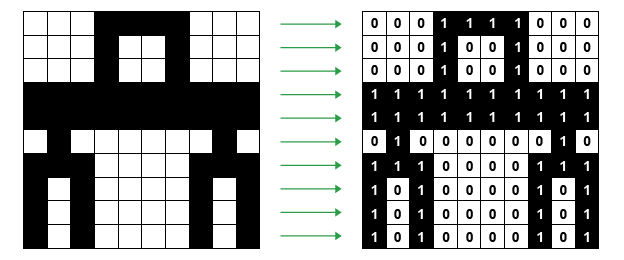
\includegraphics[scale=0.35]{Binary02.png}
\caption{Binary Images}
\end{figure}
\end{frame}

\begin{frame}{Boundary (Border) algorithm}
\begin{itemize}
\item Assume a binary image in which object and background points are labeled 1 and 0, respectively.
\item Assume images are padded with the border of 0s to avoid object merging with the image border
\end{itemize}
\begin{figure}
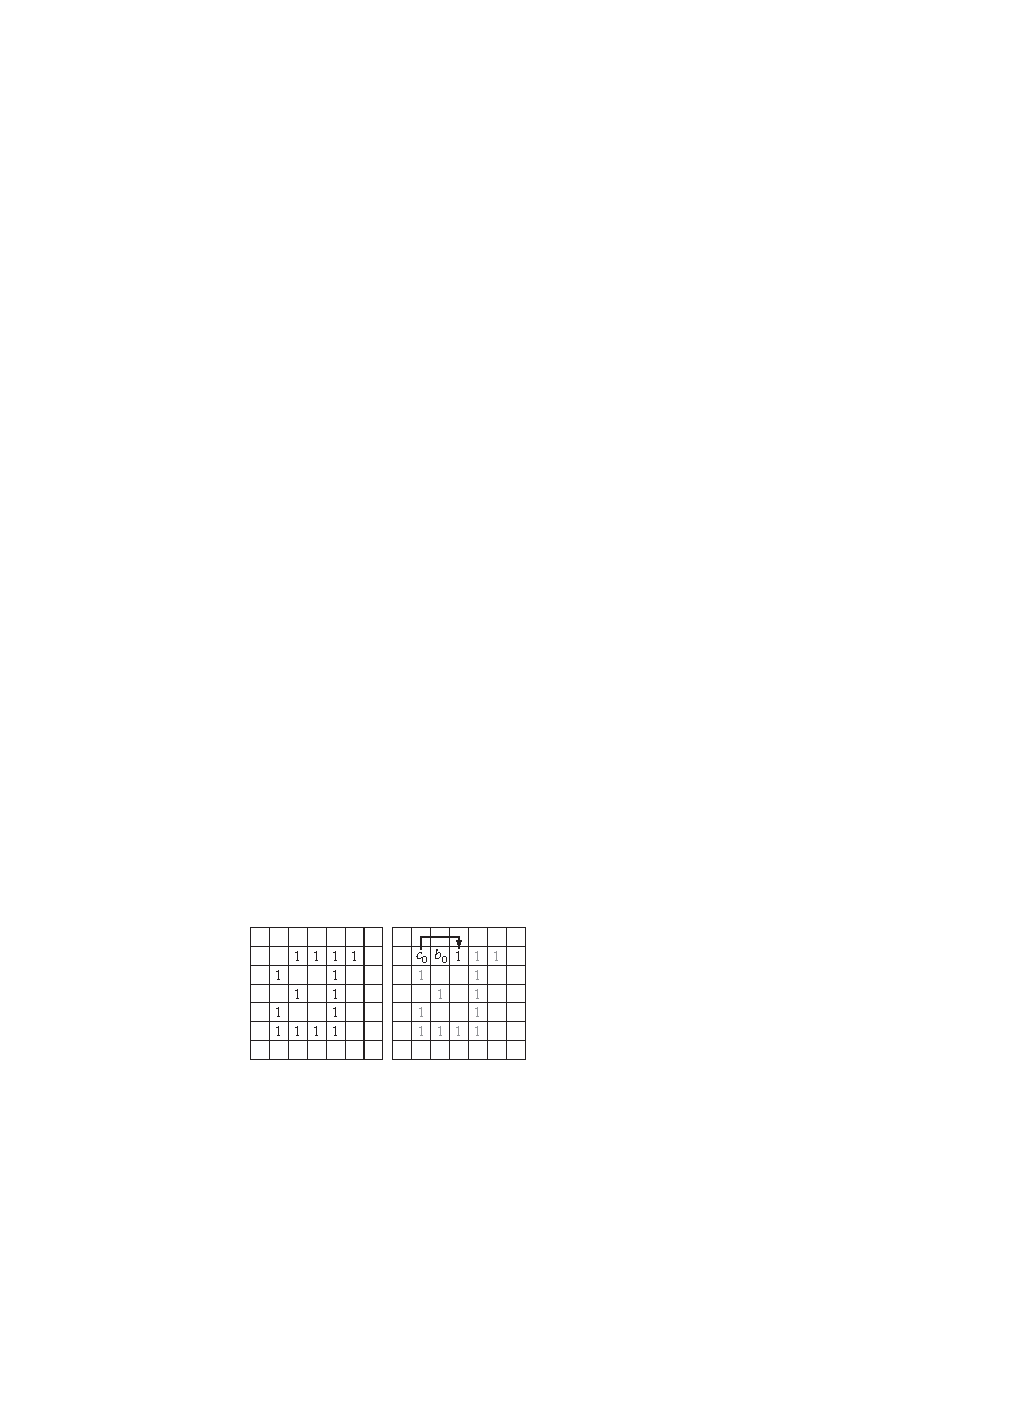
\includegraphics[scale=0.9]{Feature06}\\
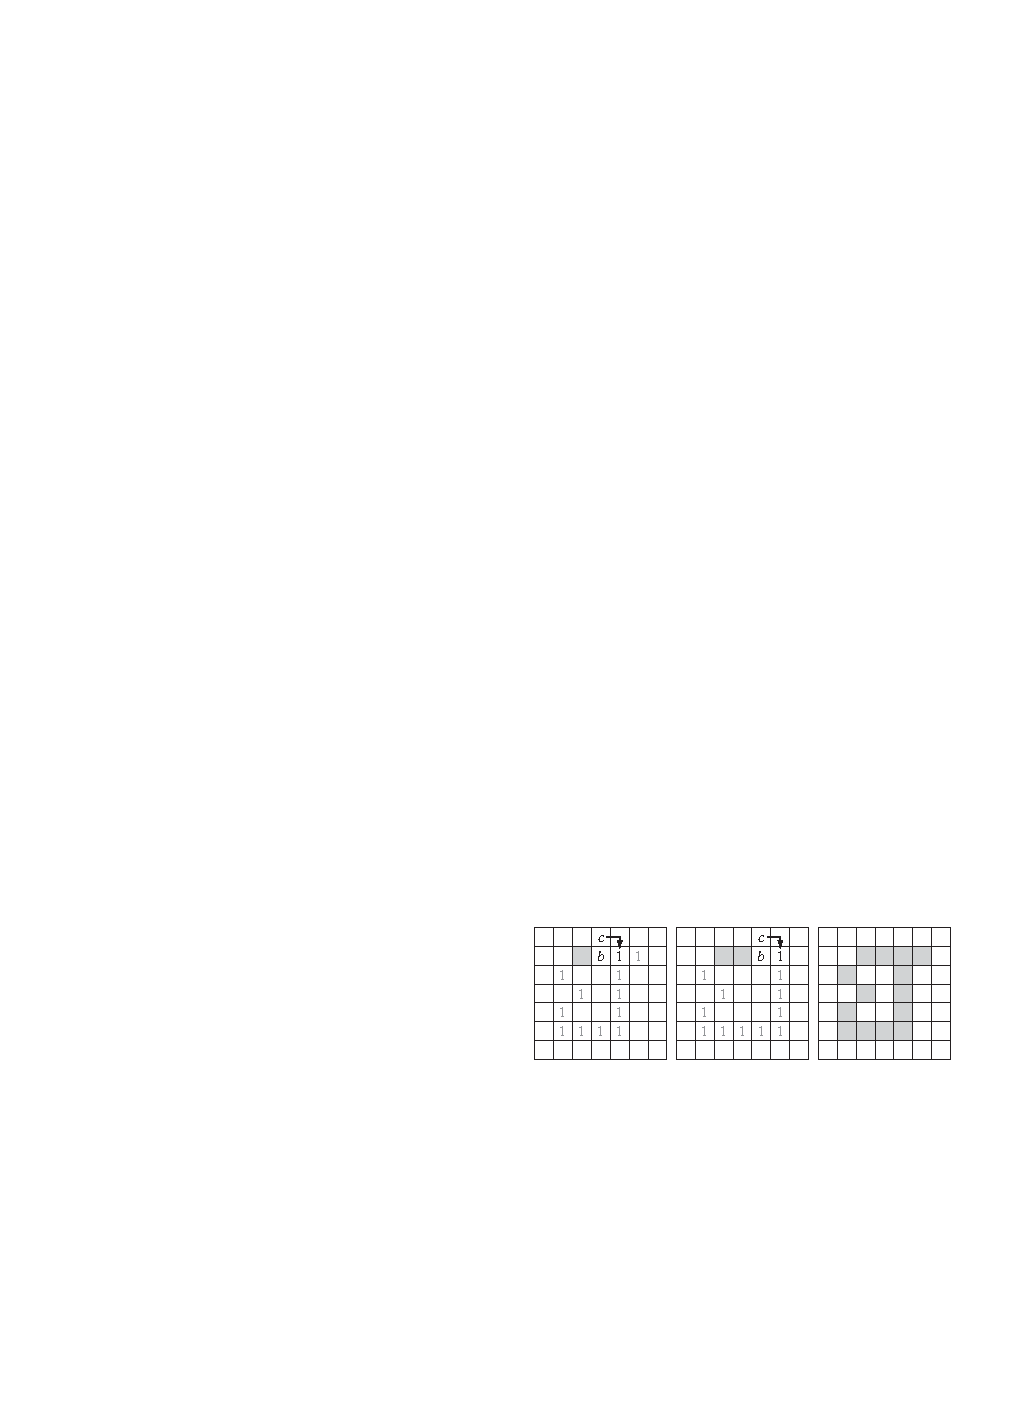
\includegraphics[scale=0.9]{Feature07}
\caption{Illustration of the first few steps in the {\color{maroon}boundary-following algorithm}}
\end{figure}
\end{frame}

\begin{frame}{Boundary algorithm (Moore boundary tracking algorithm)}
\begin{footnotesize}
\begin{itemize}
\item[1.] Let the starting point, $b_0$ be the \textit{uppermost, leftmost} point in the image that is labeled 1. Denote by $c_0$ the \textit{west} neighbor of $b_0$.
Clearly, $c_0$ always is a background point. Examine the 8-neighbors of $b_0$, starting at $c_0$ and proceeding in a clockwise direction. Let $b_1$ denote
the \textit{first} neighbor encountered whose value is 1, and let $c_1$ be the (back-ground) point immediately preceding $b_1$ in the sequence. Store the locations of $b_0$ and $b_1$ for use in Step 5.
\item[2.] Let $b=b_1$ and $c=c_1$.
\item[3.] Let the 8-neighbors of $b$, starting at $c$ and proceeding in a clockwise direction, be denoted by $n_1,n_2,\ldots,n_8$. Find the first $n_k$ labeled 1.
\item[4.] Let $b=n_k$ and $c=n_{k-1}$
\item[5.] Repeat Step 3 and 4 until $b=b_0$ and the next boundary point found in $b_1$. The sequence of $b$ points found when the algorithm stops constitutes the set of ordered boundary points.
\end{itemize}
\end{footnotesize}
\end{frame}

\begin{frame}{Boundary algorithm - stopping criterion}
\begin{figure}
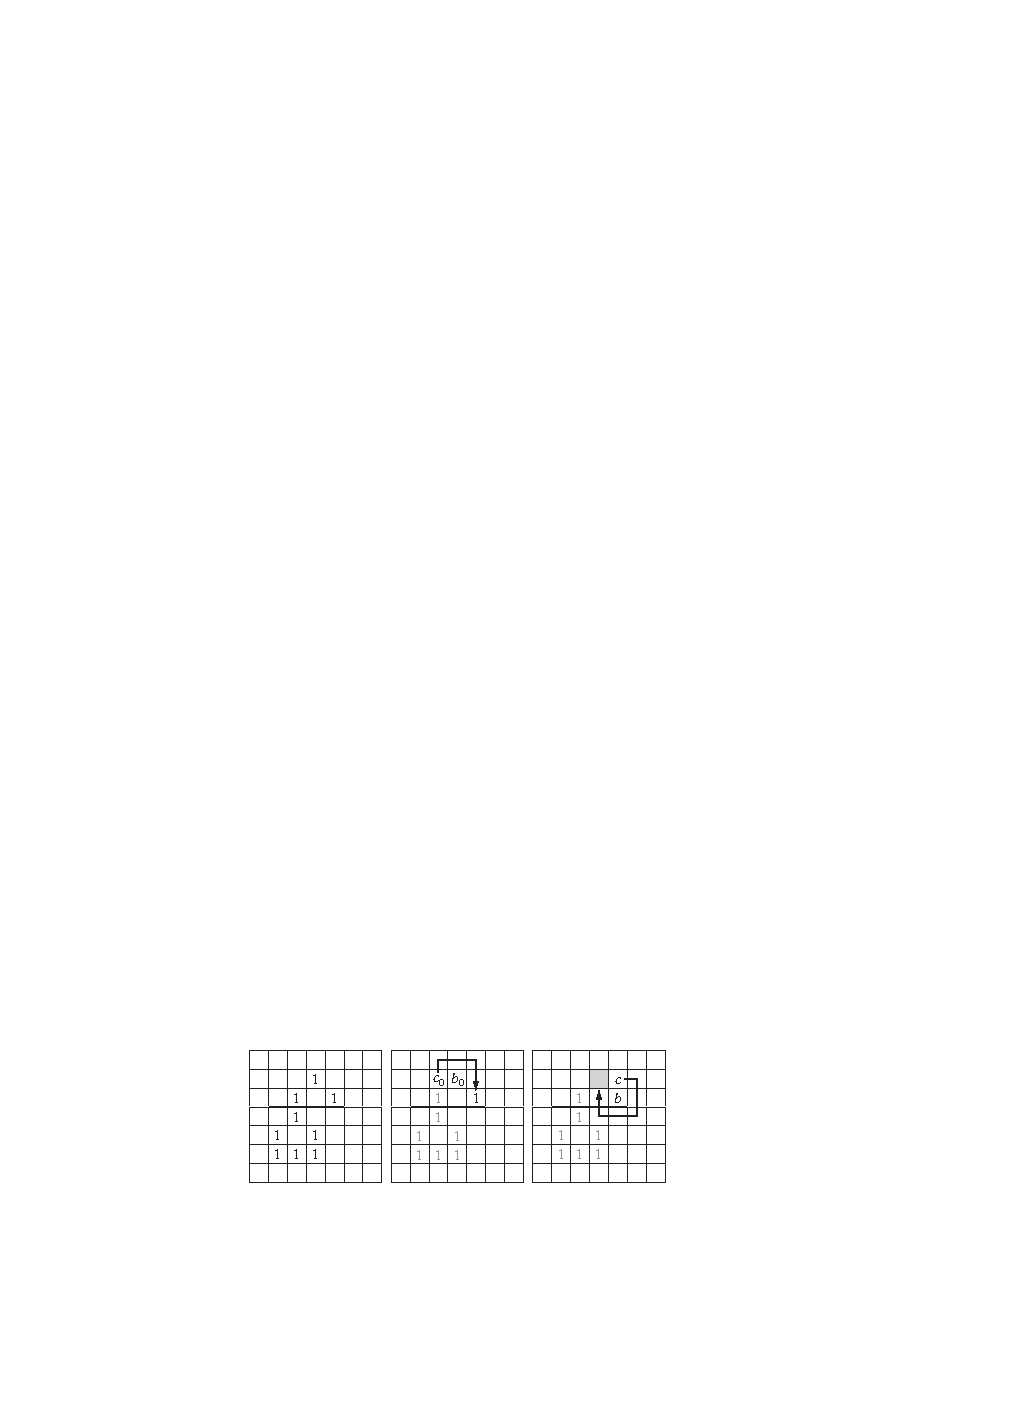
\includegraphics[scale=1.1]{Feature08}
\caption{Illustration of an erroneous result when the stopping rule is such that boundary-following stops when the starting point, $b_0$, is encountered again}
\end{figure}
\end{frame}

\begin{frame}{Boundary representation: Chain Codes}
\begin{itemize}
\item In order to represent a boundary, it is useful to compact the raw data ({\color{mycolor2}list of boundary pixels})
\item {\color{mycolor1}Chain codes:} list of segments with defined length and direction
\begin{itemize}
\item 4-directional chain codes
\item 8-directional chain codes
\end{itemize}
\begin{figure}
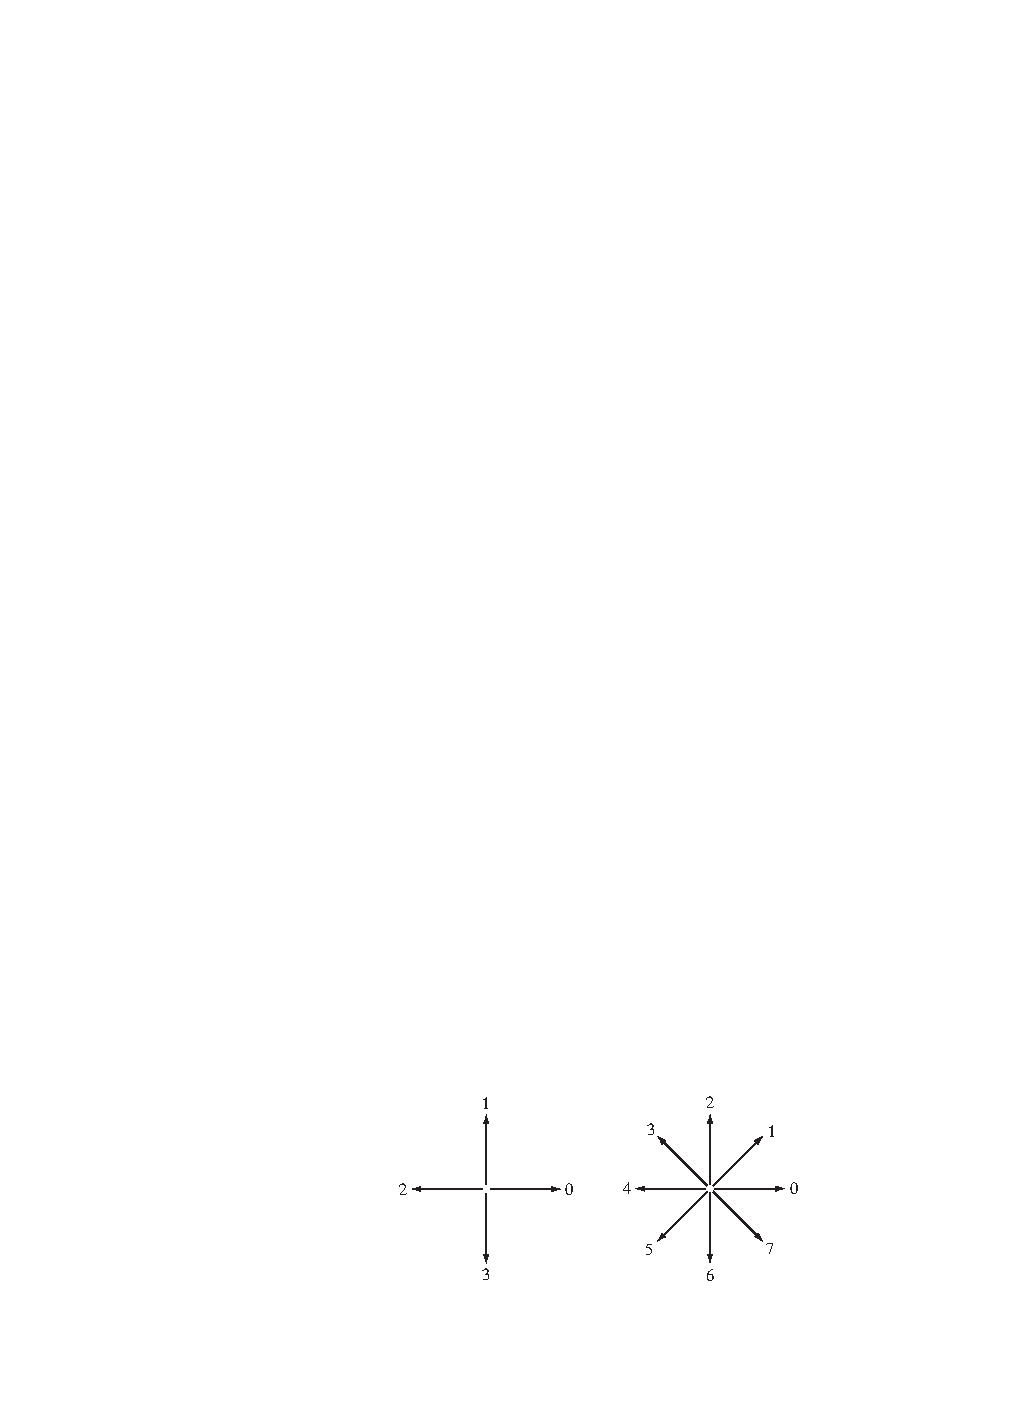
\includegraphics[scale=1]{Feature01}
\caption{Direction numbers for (a) 4-directional chain code, and (b) 8-directional chain code}
\end{figure}
\end{itemize}
\end{frame}

\begin{frame}{Boundary representation: Chain Codes}
\begin{itemize}
\item It may be useful to downsample the data before computing the chain code
\begin{itemize}
\item to reduce the code dimension
\item to remove small detail along the boundary
\end{itemize}
\begin{figure}
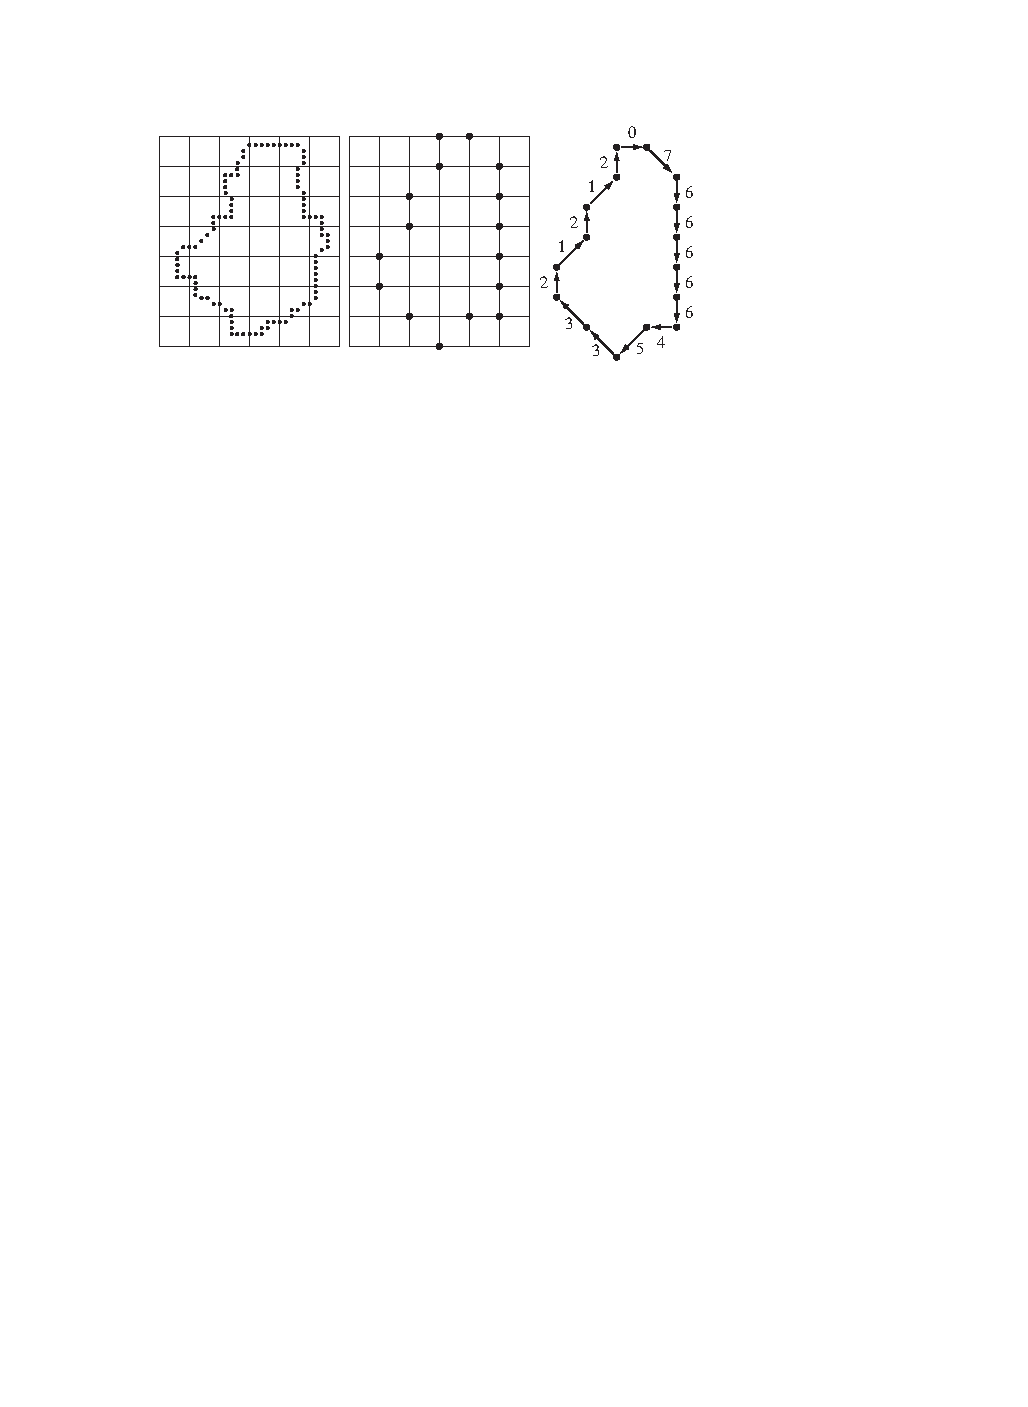
\includegraphics[scale=0.75]{Feature02}
\caption{(a) Digital boundary with resampling grid superimposed, (b) Result of resampling, (c) 8-directional chain-coded boundary.}
\end{figure}
\item Can you draw 4-directional chain-coded boundary?
\end{itemize}
\begin{tikzpicture}[remember picture,overlay]
    \node (img1) at (10.5,5.5) {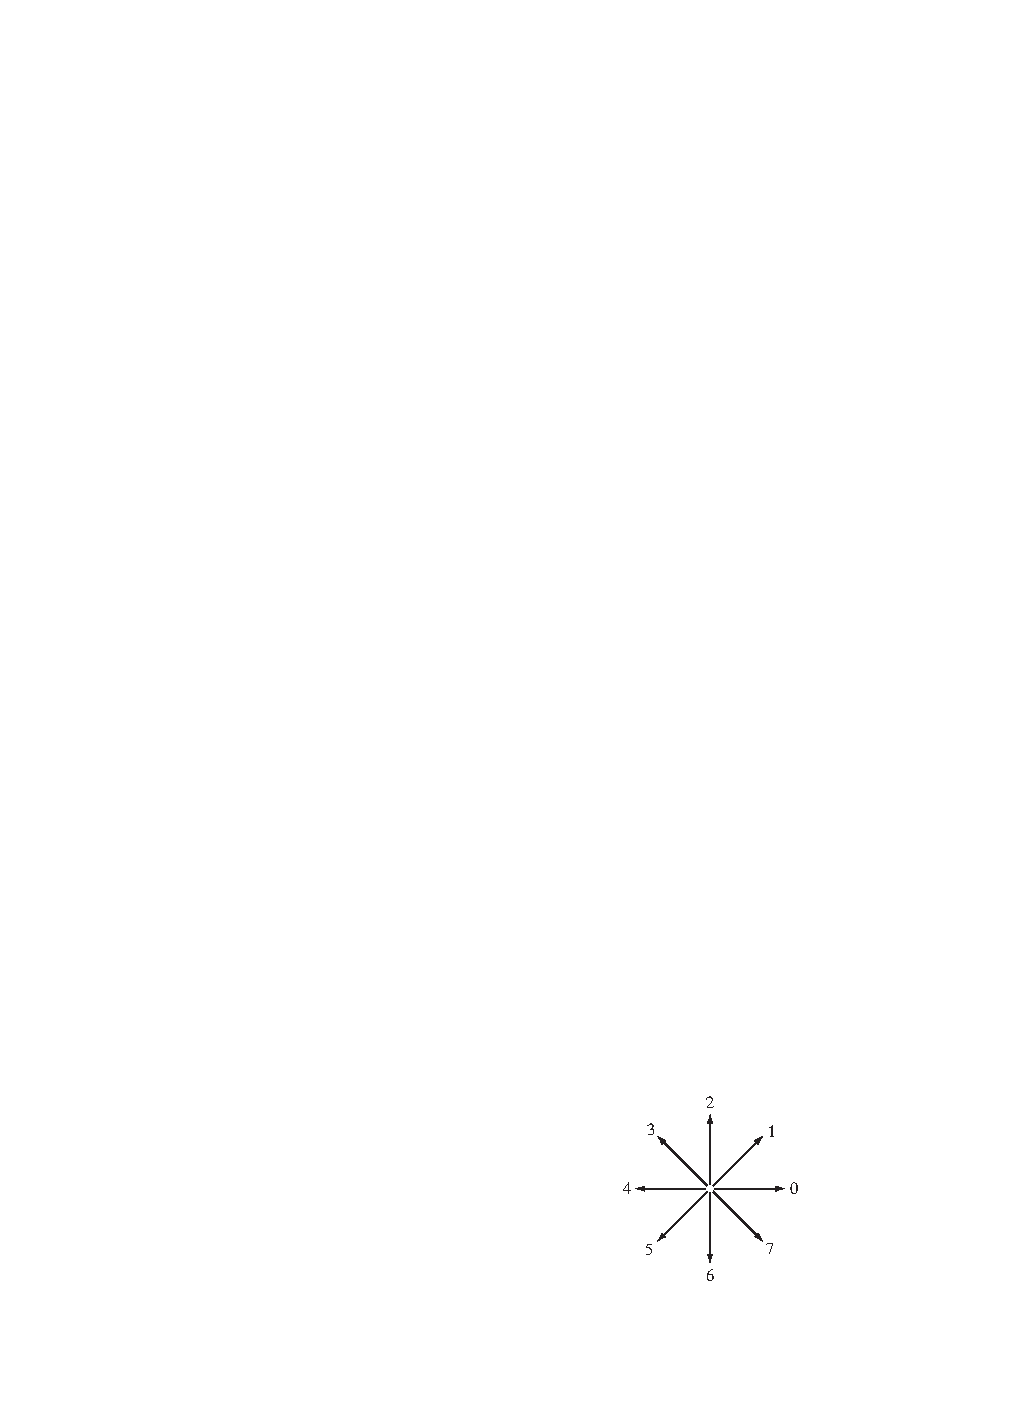
\includegraphics[scale=0.7]{Figures/Feature01a}};
\end{tikzpicture}
\end{frame}

\begin{frame}{Boundary representation: Chain Codes}
\vspace{2.3cm}
\begin{figure}
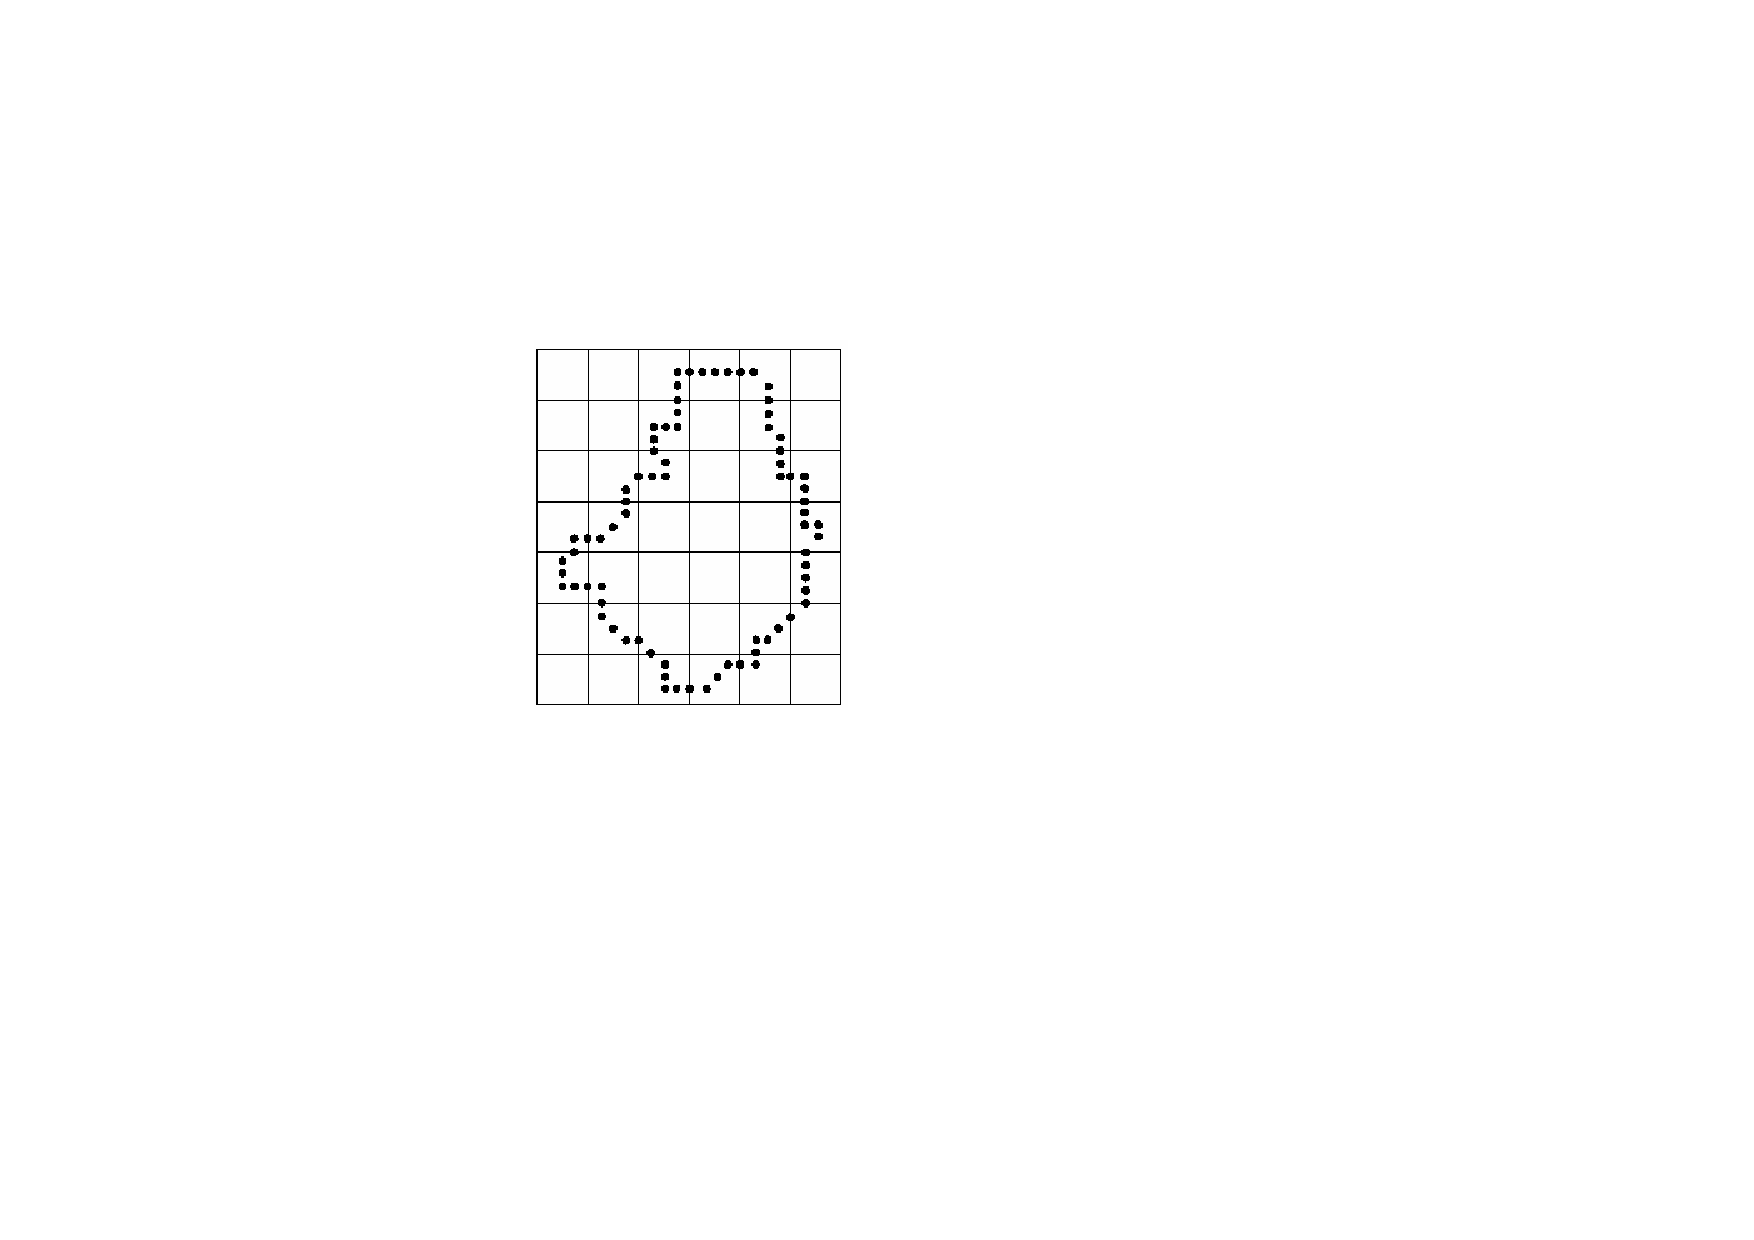
\includegraphics[scale=0.7]{Feature09}~~~
\onslide<2->{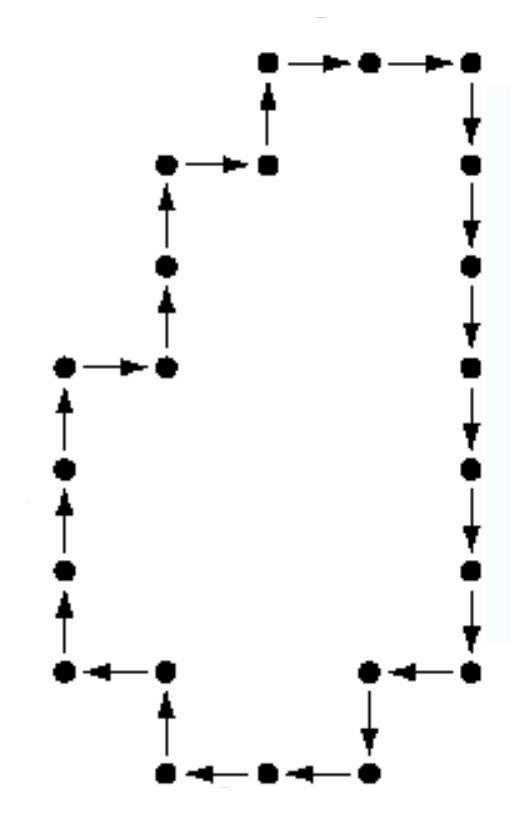
\includegraphics[scale=0.235]{Feature10_1.png}~~~}
\onslide<3->{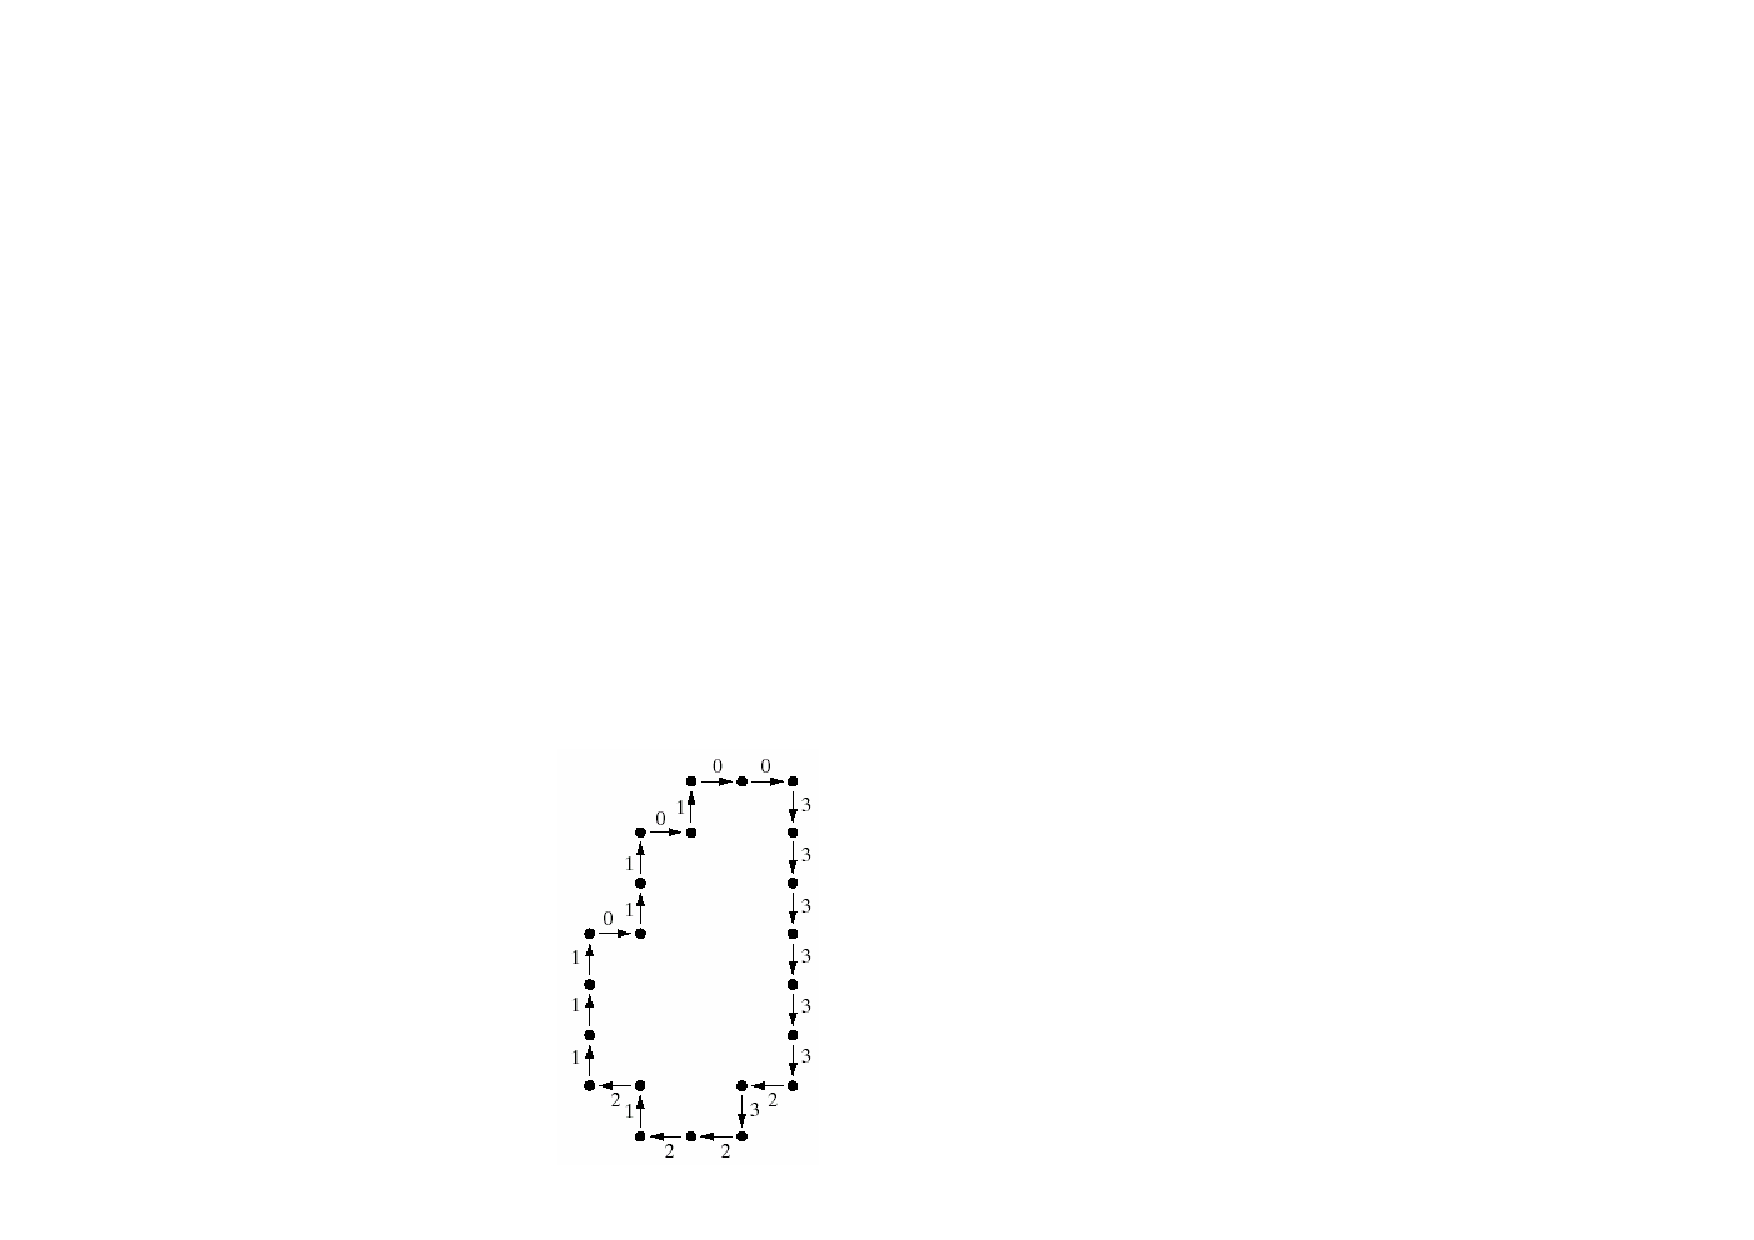
\includegraphics[scale=0.65]{Feature10}}
\end{figure}
\begin{tikzpicture}[remember picture,overlay]
\node (img1) at (2,6.5) {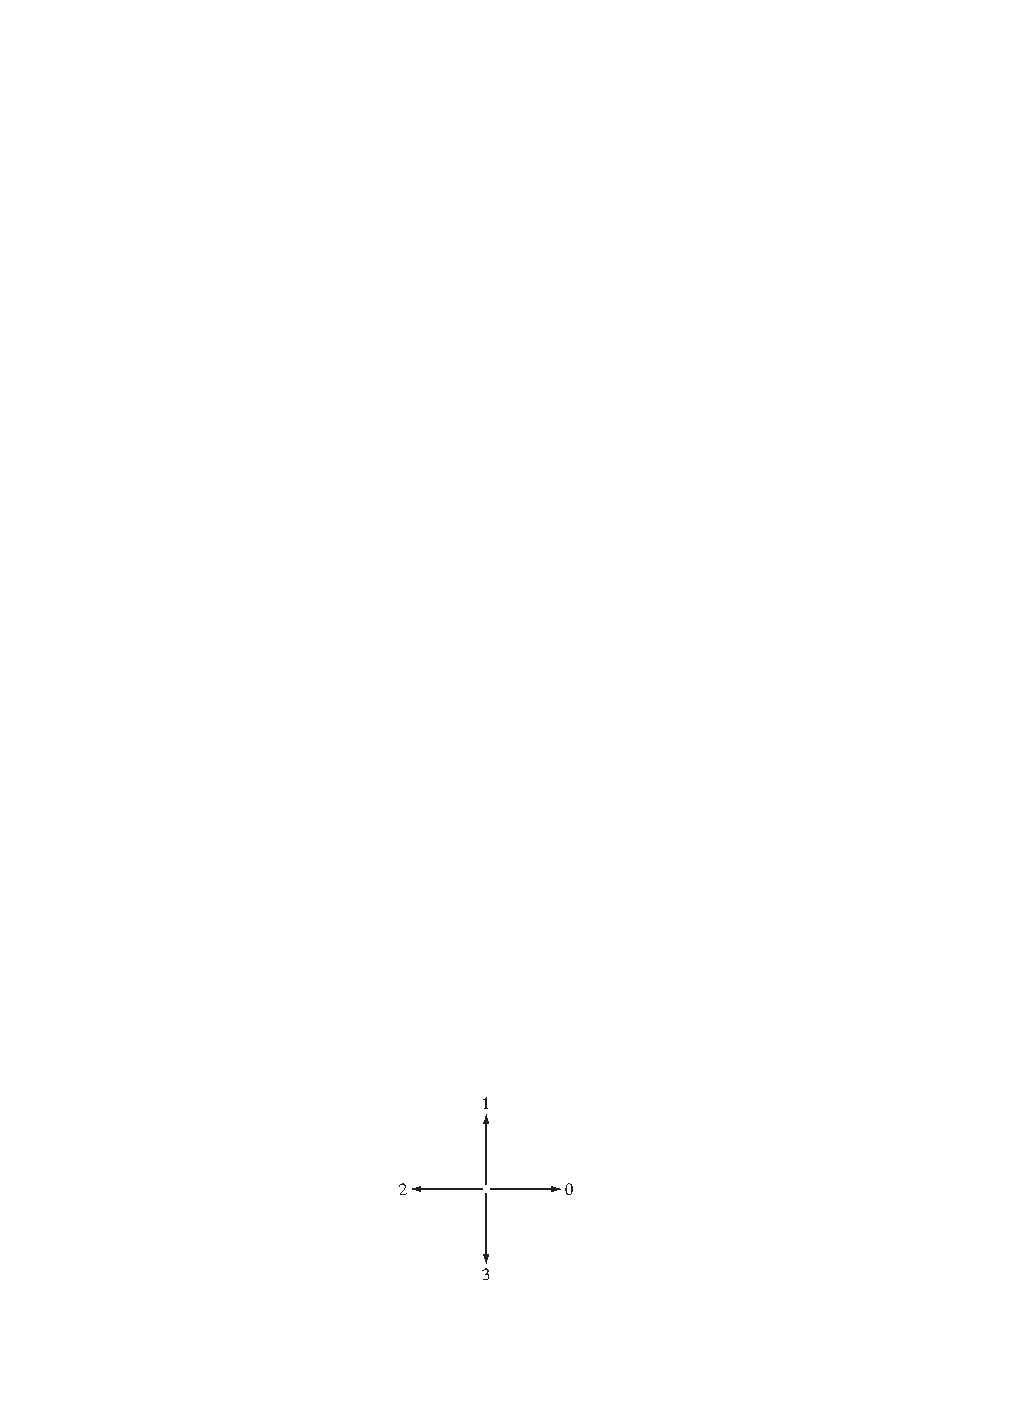
\includegraphics[scale=0.75]{Figures/Feature01b}};
\onslide<4->{\node (img1) at (7,6.5) {{\color{mycolor1}Chain code:} 0033333323221211101101};}
\end{tikzpicture}
\end{frame}

%\begin{frame}{Boundary representation: Chain Codes}
%\begin{itemize}
%\item Chain codes are used to represent a boundary by a connected sequence of straight-line segments of specified length and direction.
%\item The direction of each segment is coded by using a numbering scheme that we discussed.
%\end{itemize}
%\end{frame}

\begin{frame}{Boundary representation: Differential Chain Code}
\begin{itemize}
\item The chain code of a boundary depends on the starting point.
\begin{itemize}
\item normalize with respect to the starting point (circular sequence)
\item the new starting point is the one who gives a sequence of numbers giving the \textit{\color{mycolor1}smallest/largest integer}.
\end{itemize}
\item Normalize with respect to rotation:
\begin{itemize}
\item First difference can be used
\item E.g., $10103322\Rightarrow 3133030$ (counting CCW) and adding the last transition (circular sequence: $2\Rightarrow 1$)\\ $\Rightarrow$ 31330303 (\textit{\color{mycolor2}Differential Chain Code})\\ $\Rightarrow$ 03033133 (\textit{\color{mycolor2}Independent of starting point}, \textit{\color{mycolor1} i.e., rotation invariant})
\end{itemize}
\begin{figure}
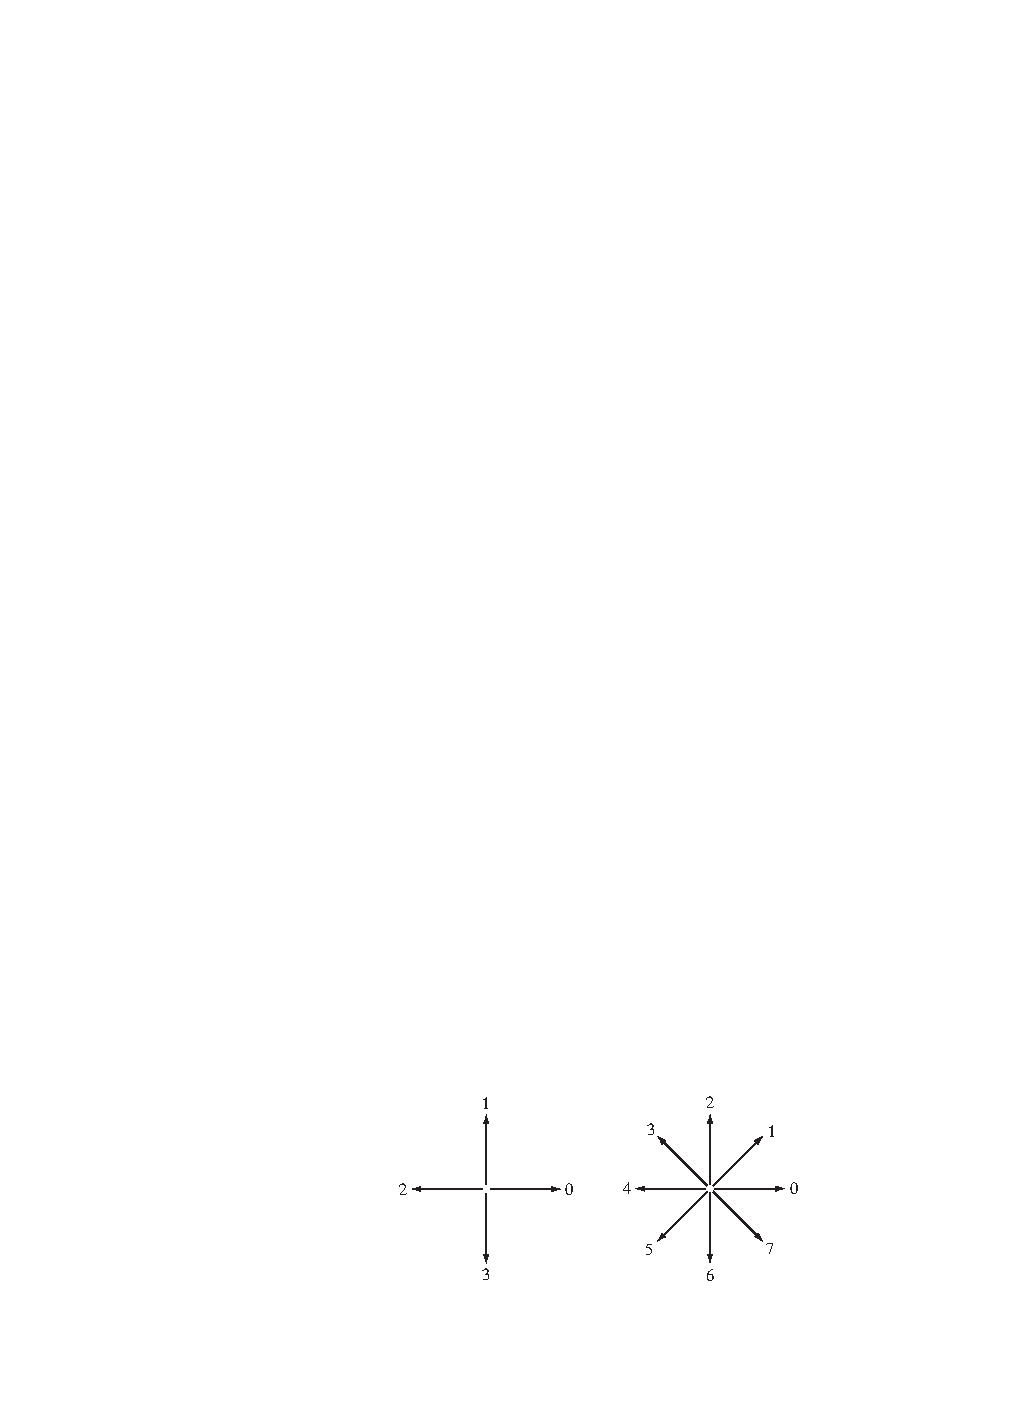
\includegraphics[scale=0.8]{Feature01}
\end{figure}
\end{itemize}
\end{frame}

\begin{frame}{Differential Chain Code}
\begin{figure}
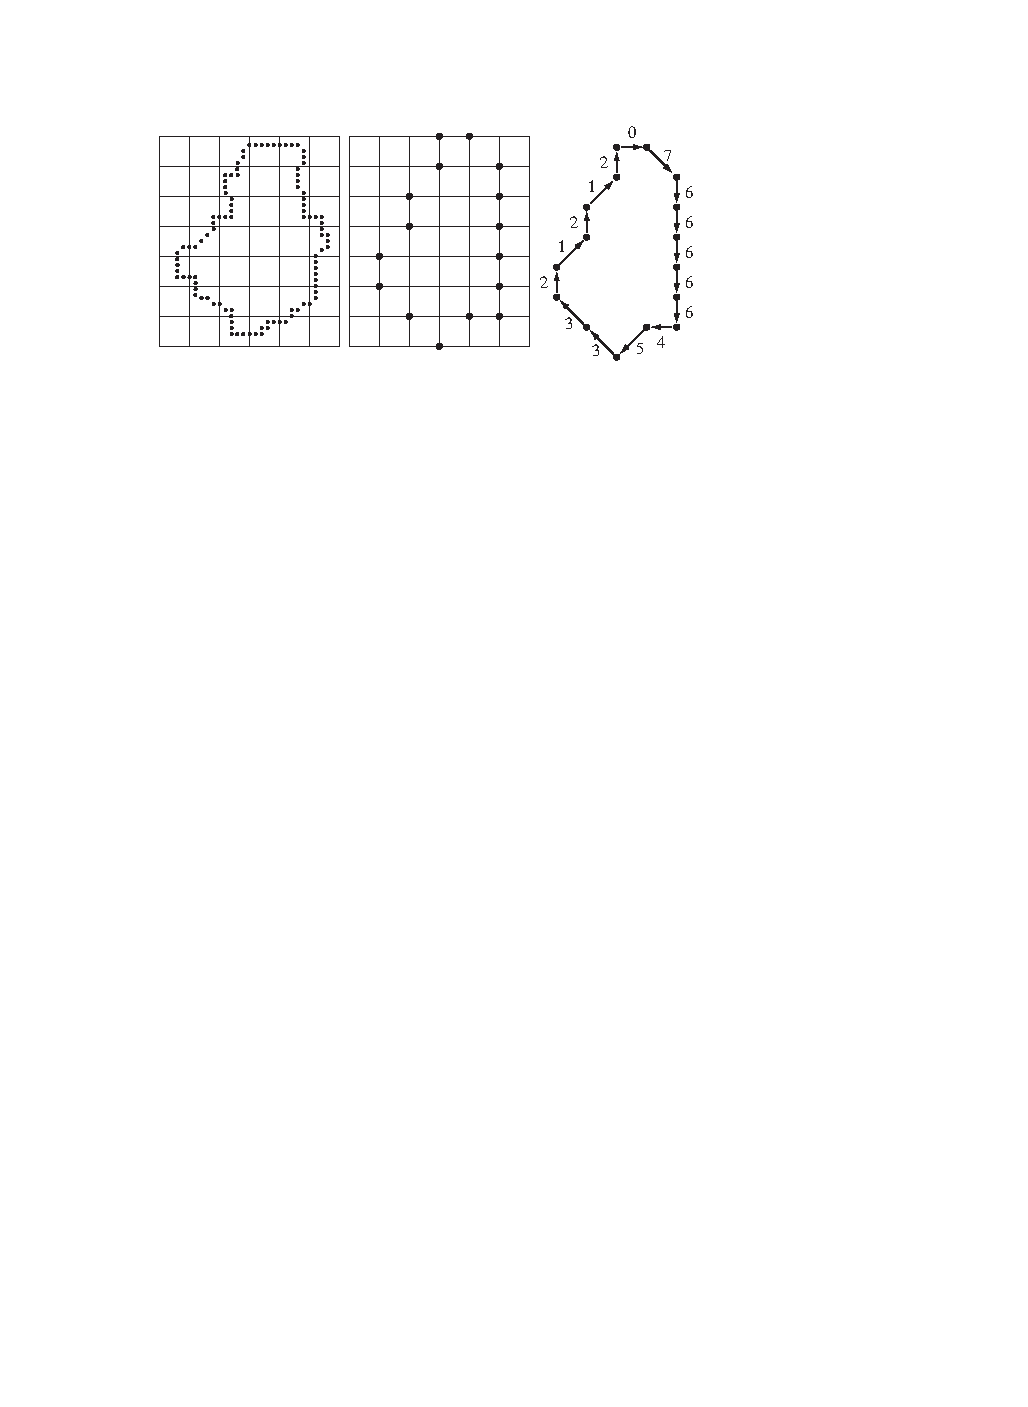
\includegraphics[scale=1]{Feature02}
\end{figure}
\onslide<1>{Can you write the Differential Chain Code?
\begin{itemize}}
\onslide<2->{\item Chain code: 0766666453321212}
\onslide<3->{\item Differential chain code: 7700006160771716}
\onslide<4->{\item Differential chain code (rotation invariant): 0000616077171677}
\end{itemize}
\end{frame}


\begin{frame}{Differential Chain Code: Validation}
\begin{figure}
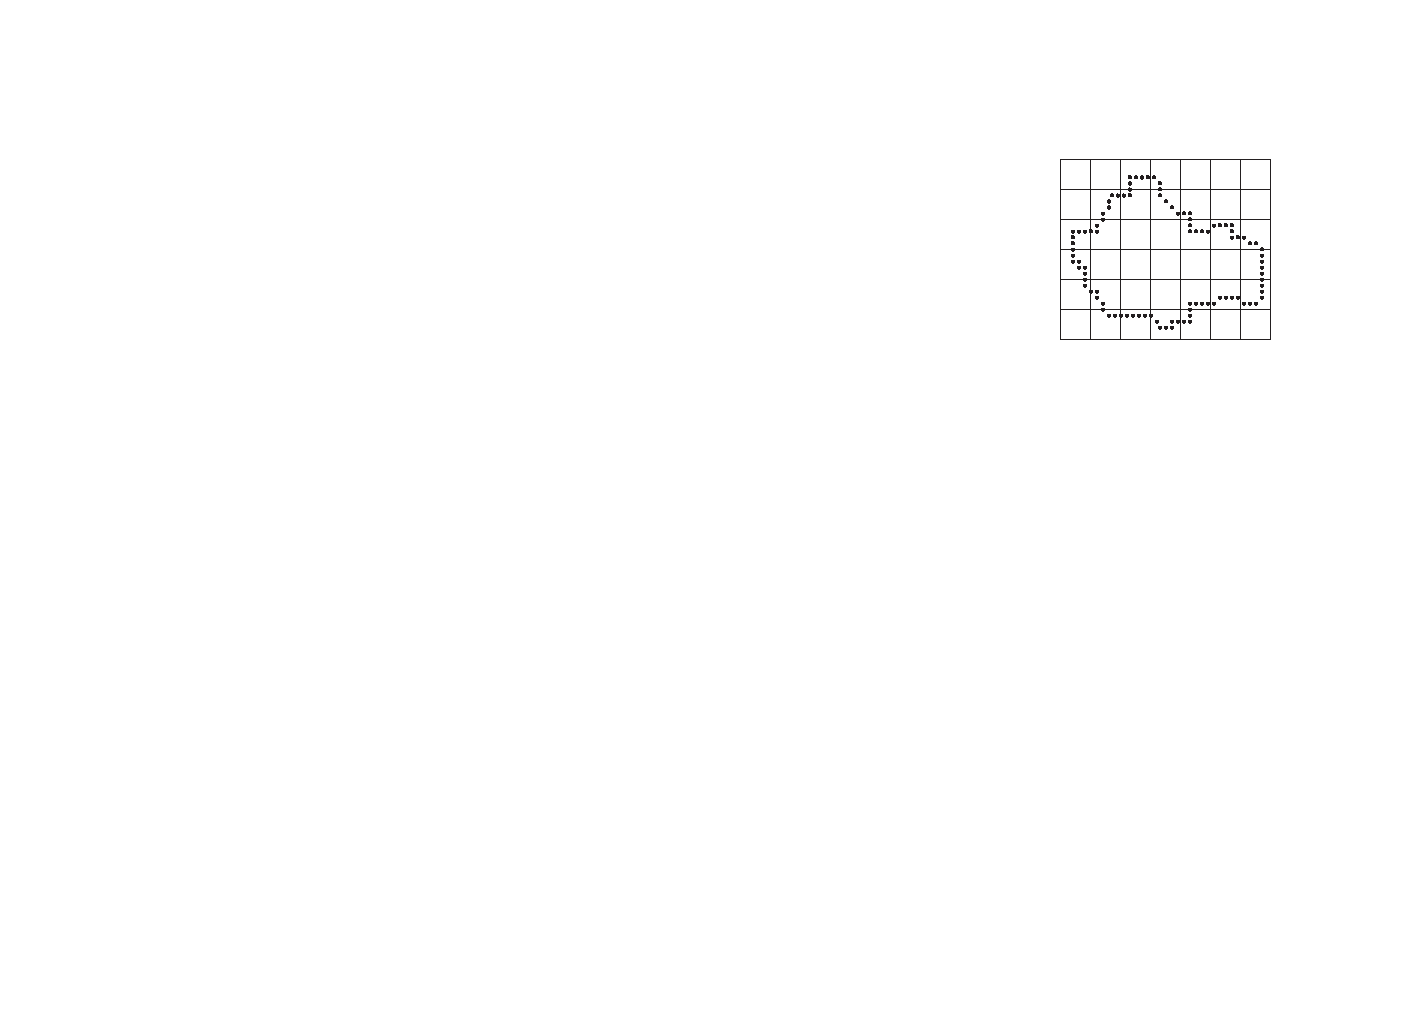
\includegraphics[scale=0.9]{Figures/Feature02a}~~~
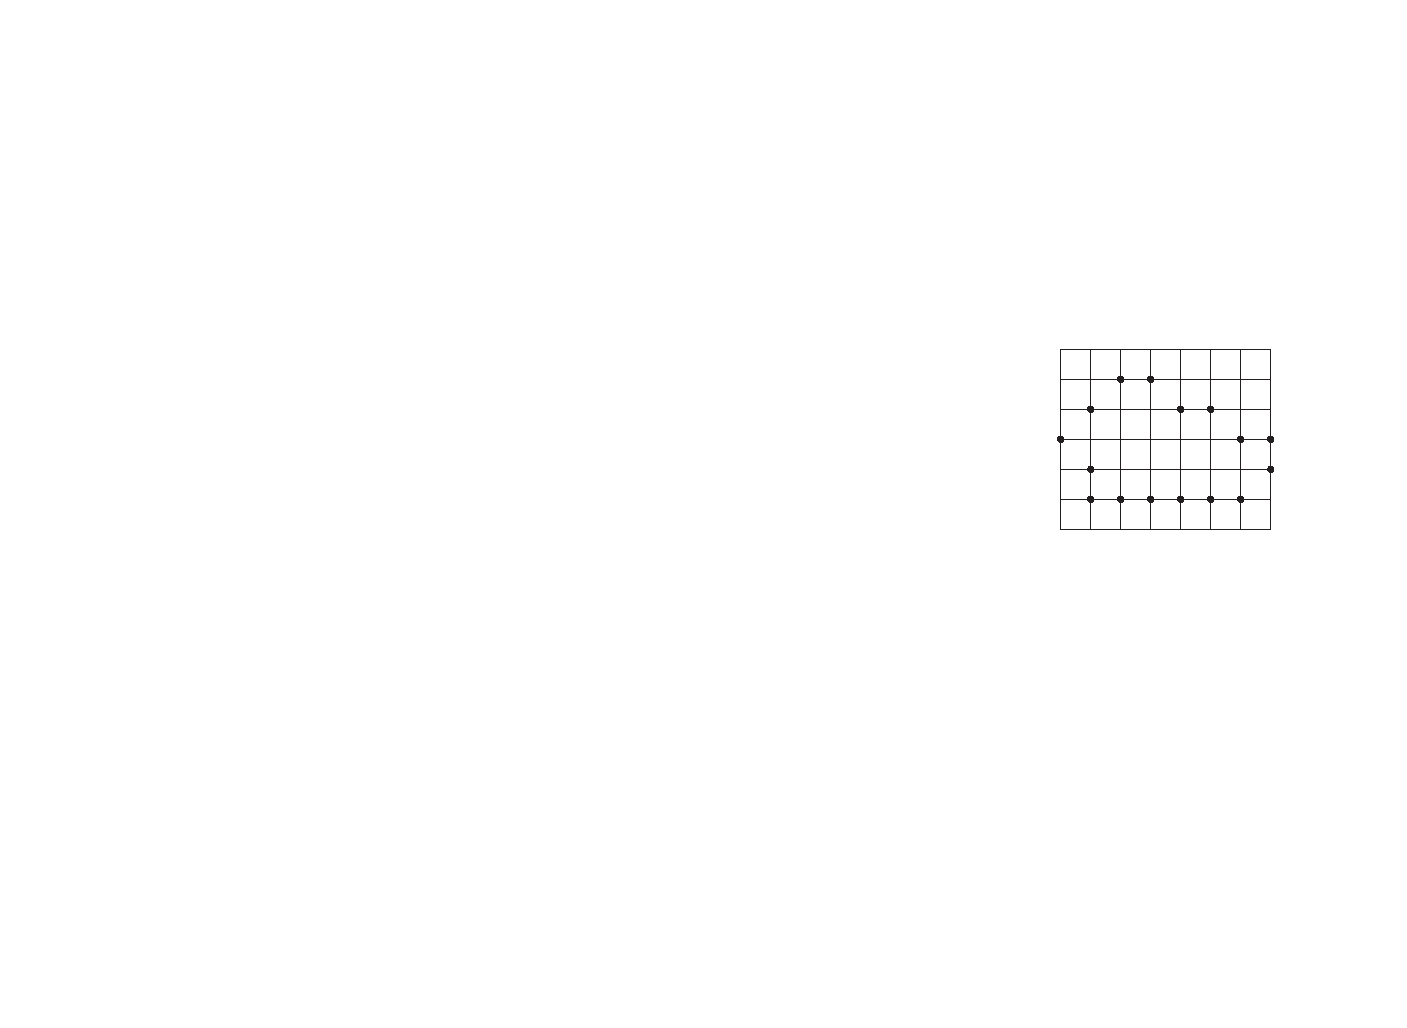
\includegraphics[scale=0.9]{Figures/Feature02b}~~~
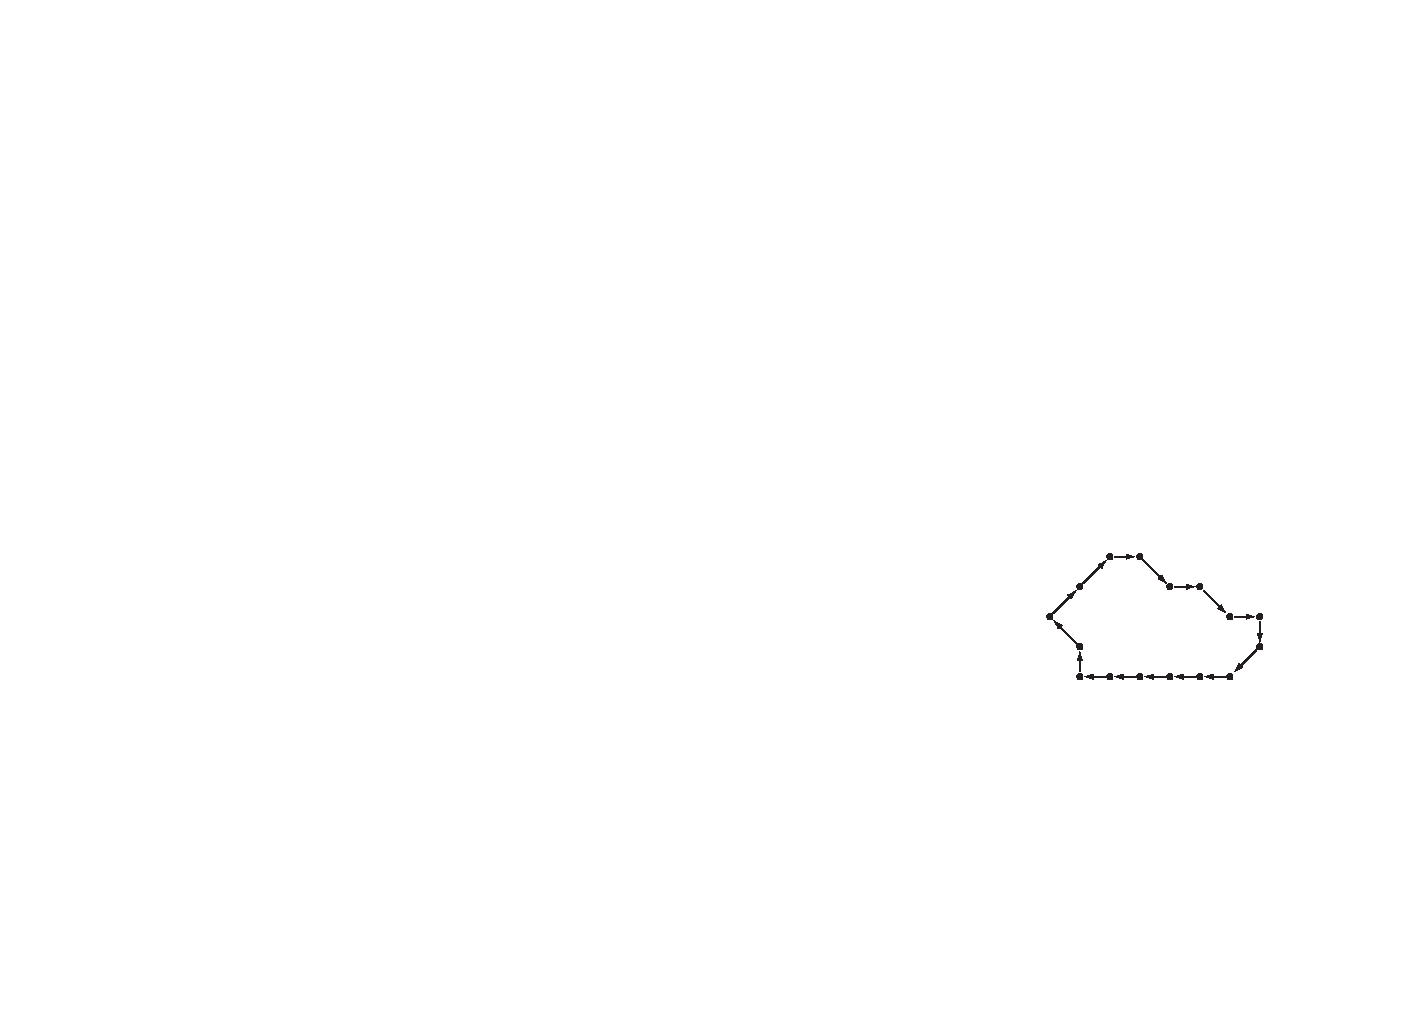
\includegraphics[scale=0.9]{Figures/Feature02c1}
\end{figure}
\onslide<1>{Can you write the Differential Chain Code?
\begin{itemize}}
\onslide<2->{\item Chain code: 0707065444442311}
\onslide<3->{\item Differential chain code: 7171677000061607}
\onslide<4->{\item Differential chain code: 0000616077171677 (validated)}
\onslide<5->{\item Is the differential chain code is invariant to rotation at any angle? ({\color{mycolor2}HW})}
\end{itemize}
\end{frame}

%\begin{frame}{Polygonal Approximation: Minimum-Perimeter polygon}
%\begin{figure}
%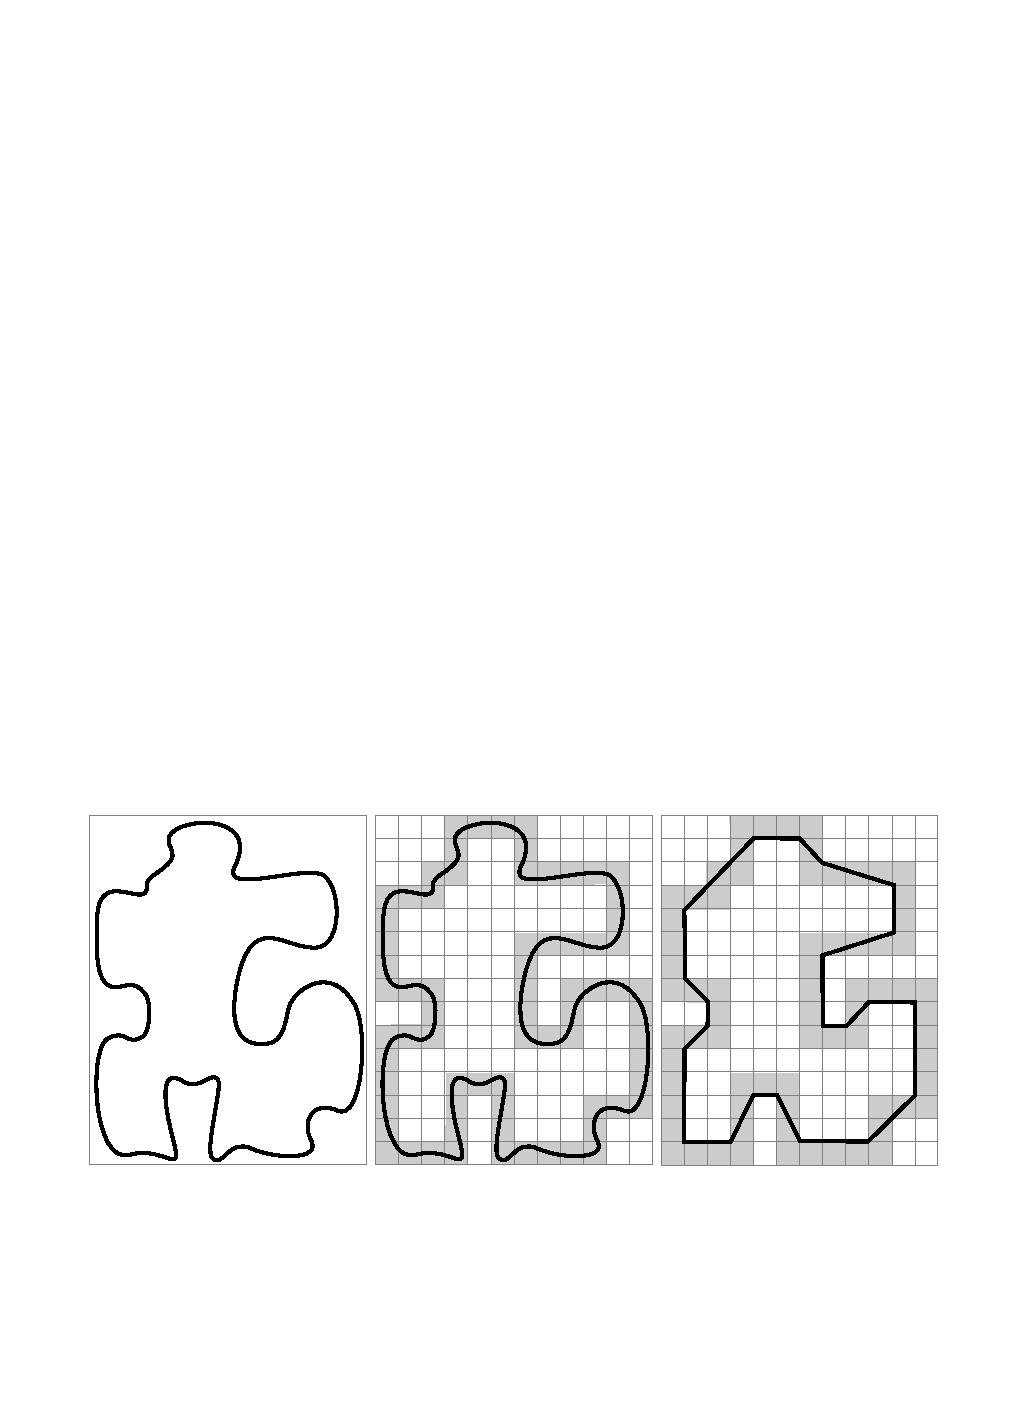
\includegraphics[scale=0.7]{Feature03}
%\end{figure}
%\end{frame}

\begin{frame}{Polygonal Approximation}
\begin{itemize}
\begin{small}
\item A digital boundary can be approximated with arbitrary accuracy by a polygon.
\item In practice, the goal of polygonal approximation is to capture the ``essence'' of the {\color{mycolor1}boundary shape} with the {\color{mycolor3}fewest possible polygonal segments}.
\begin{itemize}
\item Minimum-perimeter polygon
\item Splitting technique
\end{itemize}
\end{small}
\end{itemize}
\begin{figure}
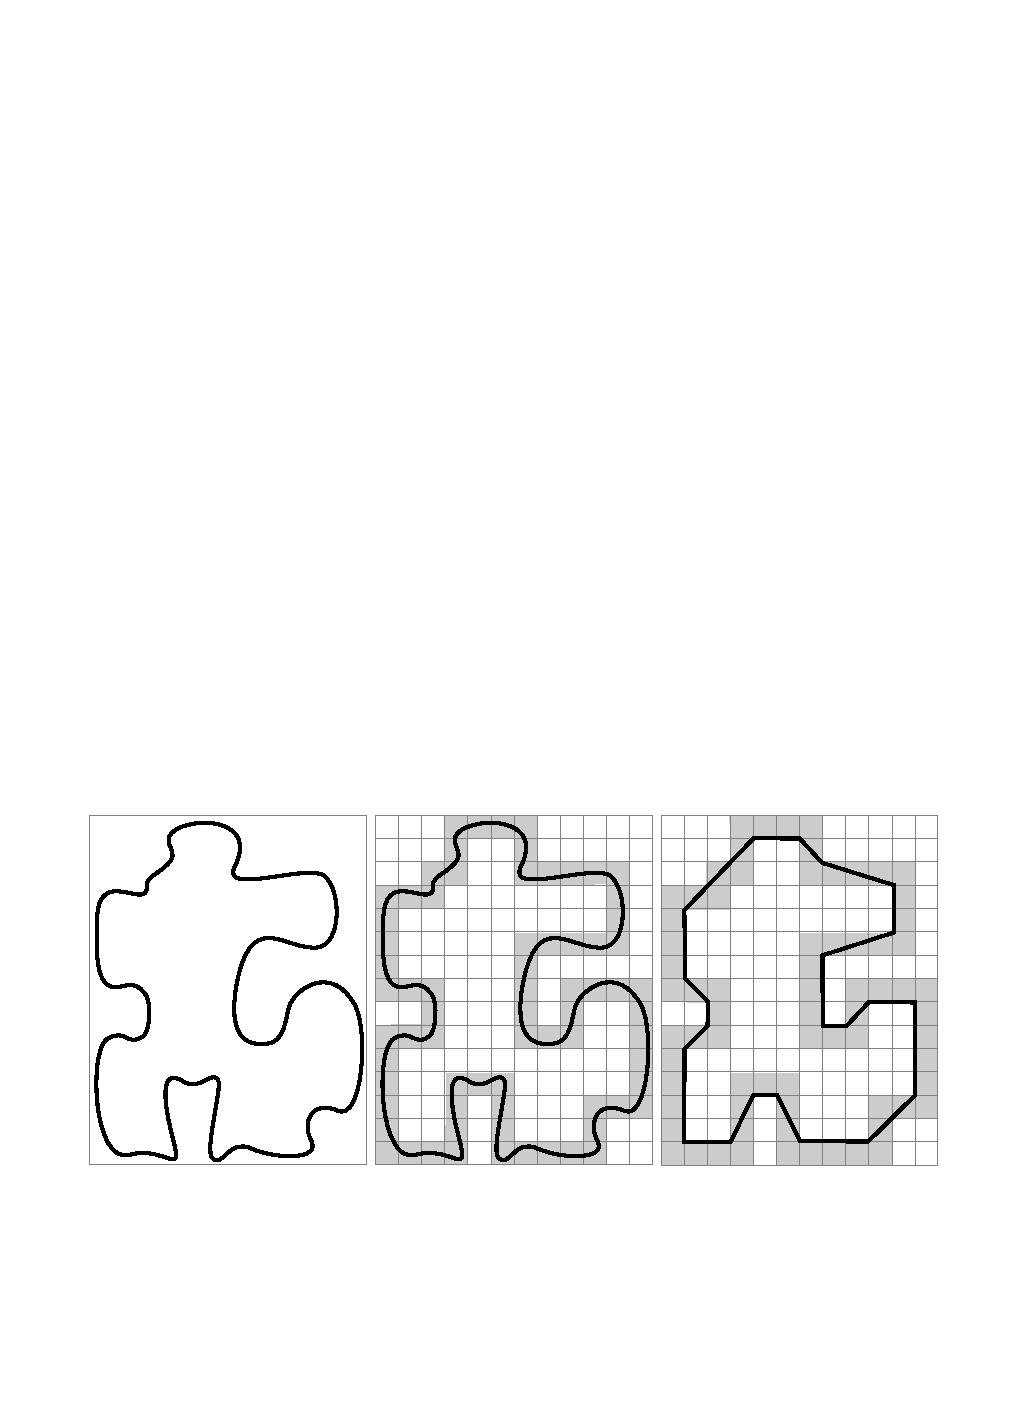
\includegraphics[scale=0.43]{Feature03}
\caption{(a) An object boundary (black curve). (b) Boundary enclosed by cells (in gray). (c) Minimum-perimeter polygon obtained by allowing the boundary to shrink. The vertices of the polygon are created by the corners of the inner and outer walls of the gray region.}
\end{figure}
\end{frame}

\begin{frame}{Polygonal Approximation: Minimum-Perimeter Polygon}
\begin{figure}
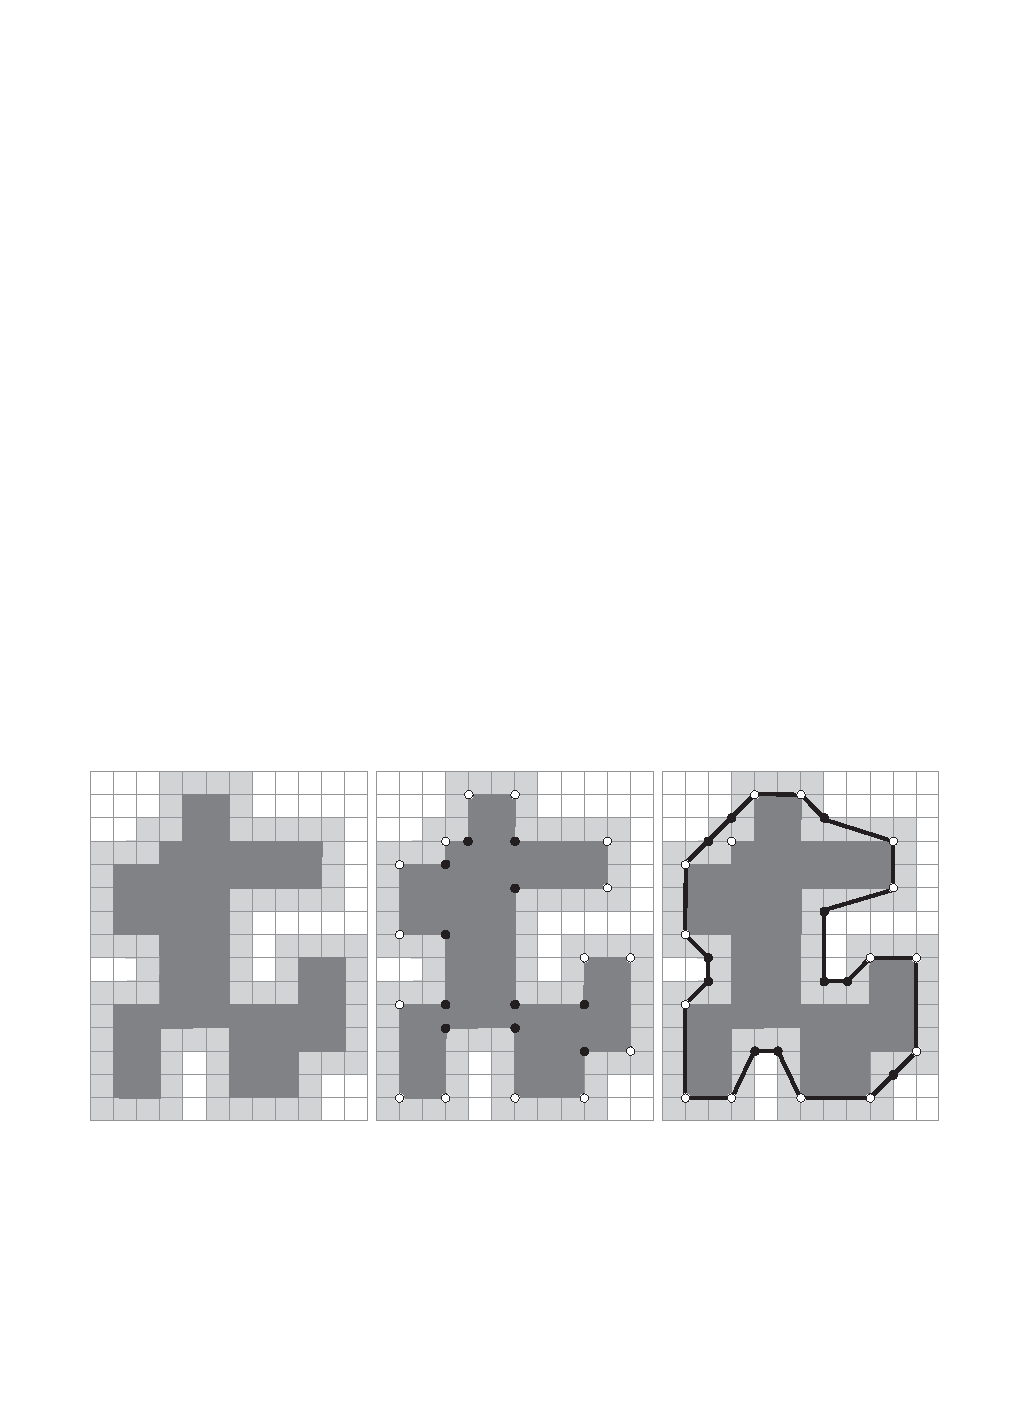
\includegraphics[scale=0.75]{Feature11}
\caption{(a) Region (dark gray) resulting from enclosing the original boundary by cells.
(b) Convex (white dots) and concave (black dots) vertices obtained by following the boundary of the dark
gray region in the counterclockwise direction. (c) Concave vertices (black dots) displaced to their diagonal
mirror locations in the outer wall of the bounding region; the convex vertices are not changed. The MPP
(black boundary) is superimposed for reference.}
\end{figure}
\end{frame}

\begin{frame}{Polygonal Approximation: Splitting Technique}
\begin{itemize}
\item One approach to boundary segment splitting is 
to subdivide a segment successively into two 
part until a \textit{\color{mycolor1}specified criterion} is satisfied.
\begin{figure}
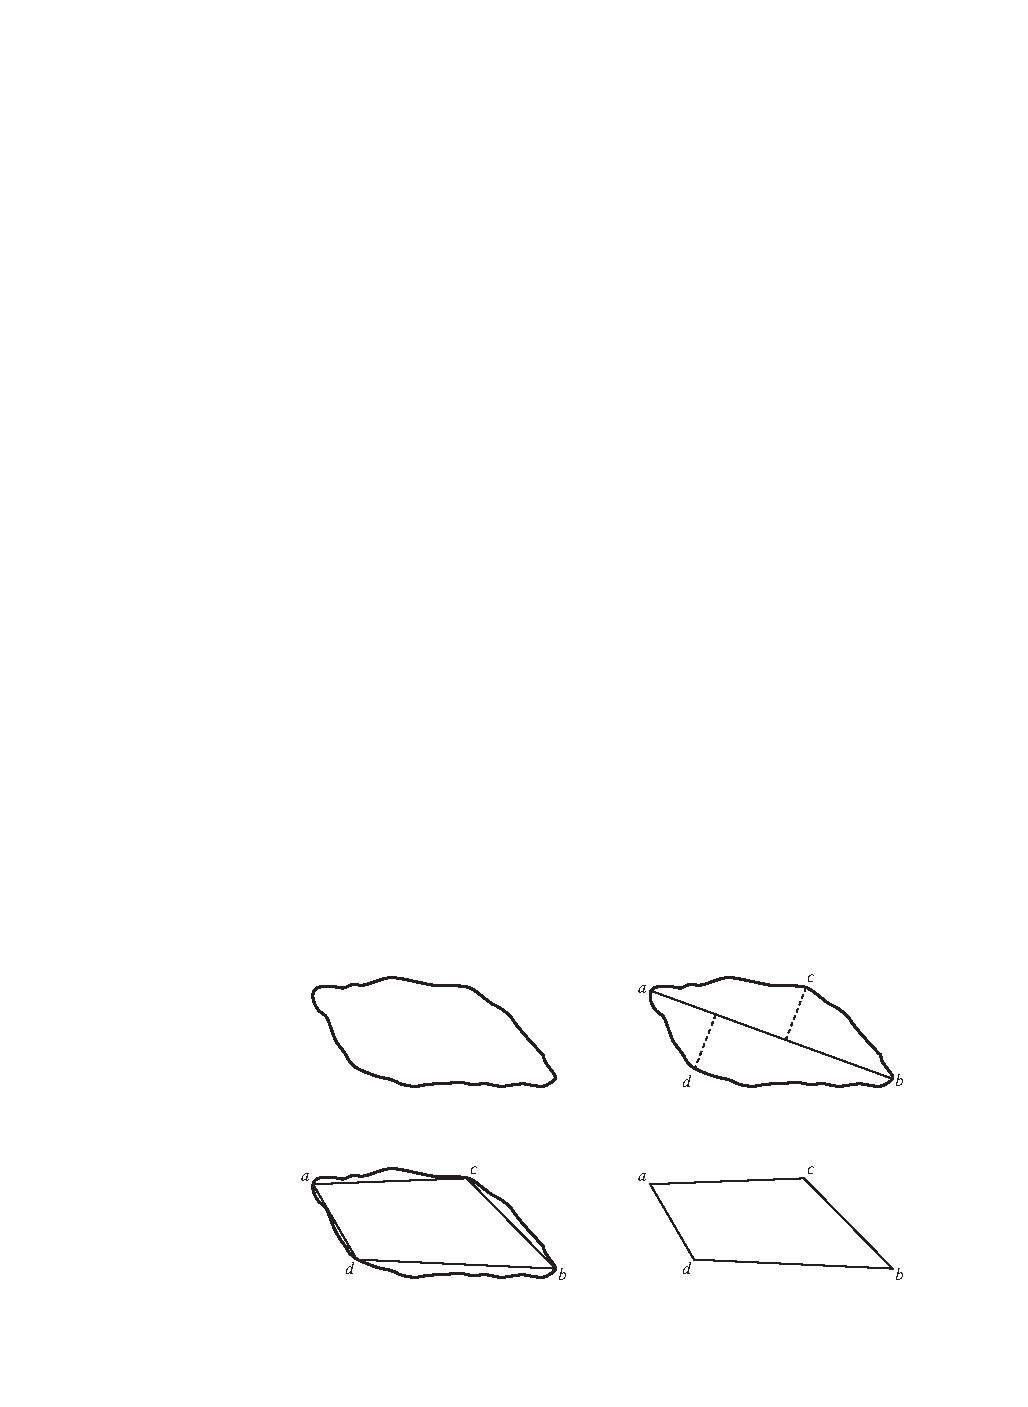
\includegraphics[scale=0.7]{Ch0001}
\caption{(a) Original boundary, (b) Boundary divided into segments based on extreme points, (c) Joining of vertices, (d) Resulting polygon}
\end{figure}
\end{itemize}
\end{frame}

\begin{frame}{Polygonal Approximation: Splitting Technique}
\begin{itemize}
\item For a closed boundary, the best starting points 
usually are two farthest points in the boundary.
\item Farthest point can be obtained by \textit{\color{mycolor1}Karhunen-Loeve transform (KLT)}.
\item The maximum perpendicular distance from a boundary segment to the line joining its two end points not exceed a preset threshold.
\item Splitting procedure with a threshold equal to 
0.25 times the length of line $ab$.
\end{itemize}
\end{frame}

\begin{frame}{Signatures}
\begin{itemize}
\item A signature is a 1-D representation of a boundary (which is a 2-D thing): it should be easier to describe.\\ e.g., distance form the centroid vs angle.
\begin{figure}
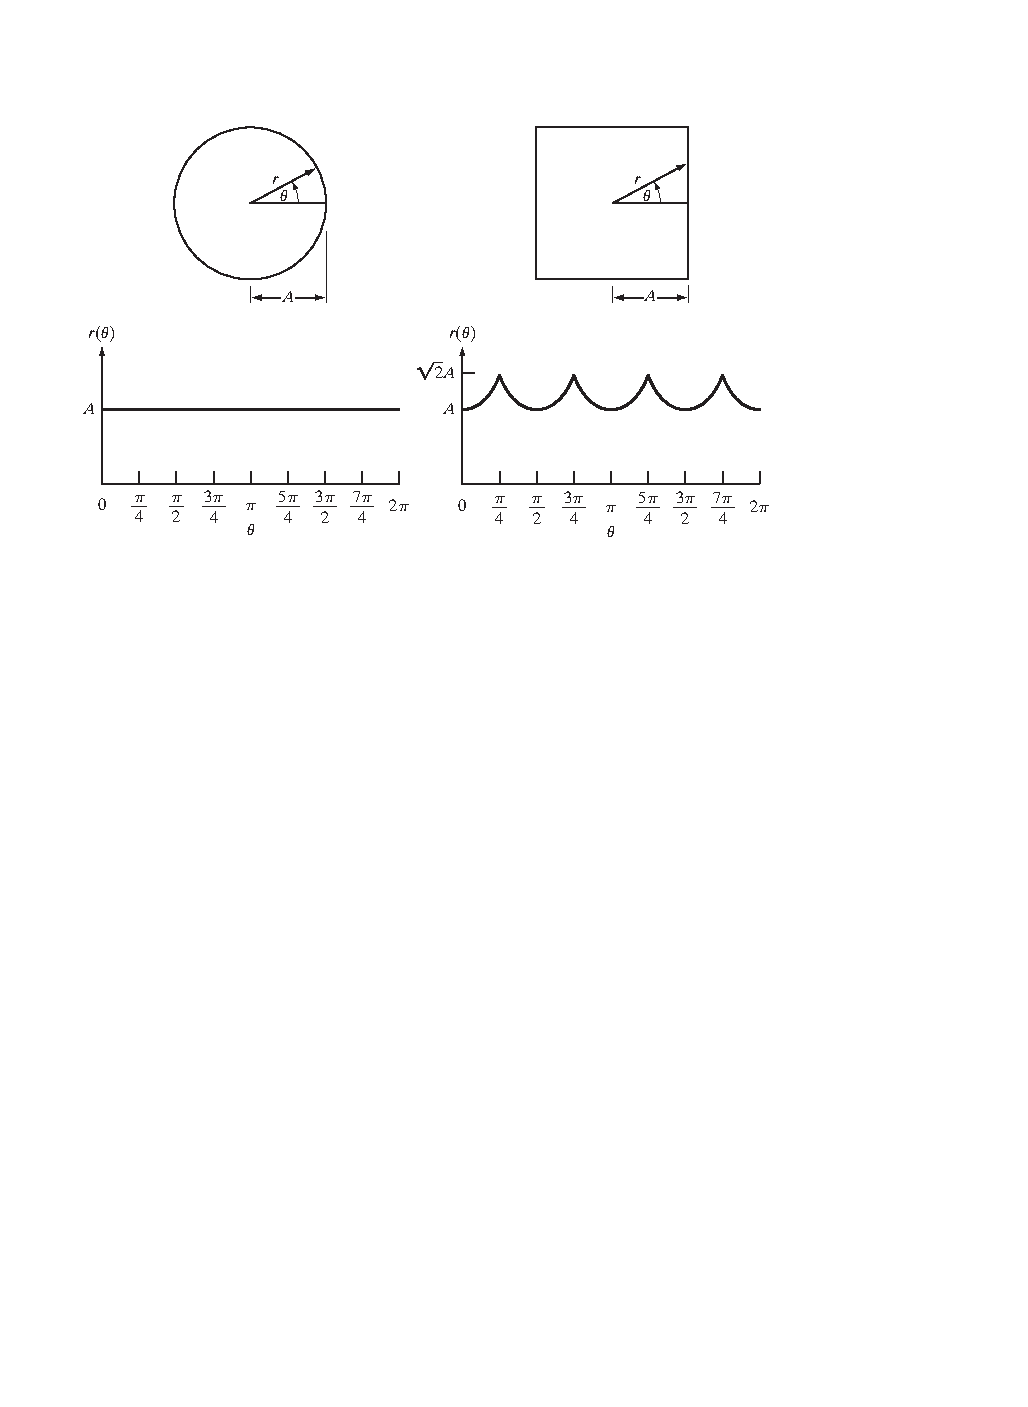
\includegraphics[scale=0.6]{Ch0002}
\caption{Distance-versus-angle signatures. (a) $r(\theta)$, is constant, (b) the signature consists of repetitions of the pattern $r(\theta)=Asec(\theta)$ for $0\leq \theta \leq \pi/4$ and $r(\theta)=Acsc(\theta)$ for $\pi/4<\theta\leq \pi/2$}
\end{figure}
\end{itemize}
\end{frame}

\begin{frame}{Signatures}
\begin{itemize}
\setlength{\itemsep}{12pt}
\item Signatures are invariant to translation, but variant to rotation.
\item Invariant to rotation: depends on the starting point
\begin{itemize}
\item the starting point could be the farthest point from the \textit{\color{mycolor1}centroid}. 
\end{itemize}
\item Scaling varies the amplitude of the signature
\begin{itemize}
\item invariance can be obtained by normalizing between 0 and 1, or
\item by dividing by the variance of the signature (does not work on circle)
\end{itemize}
\end{itemize}
\end{frame}

\begin{frame}{Boundary Segments}
\begin{itemize}
\item Decomposing a boundary into segments often 
is useful.
\item Decomposition reduces the boundary's 
complexity and thus simplifies the description 
process.
\item In this case use of the \textit{\color{mycolor1}convex hull} of the region 
enclosed by the boundary is a powerful tool for 
robust decomposition of the boundary.
\end{itemize}
\end{frame}

\begin{frame}{Boundary Segments}
\begin{itemize}
\item \textit{\color{mycolor1} Convex hull} $H$ of an arbitrary set $S$ is the 
smallest convex set containing $S$.
\item The set difference $H-S$ is called the \textit{\color{mycolor1} convex 
deficiency} $D$ of the set $S$.
\item Note that in principle, this scheme is 
independent of region size and orientation.
\end{itemize}
\begin{figure}
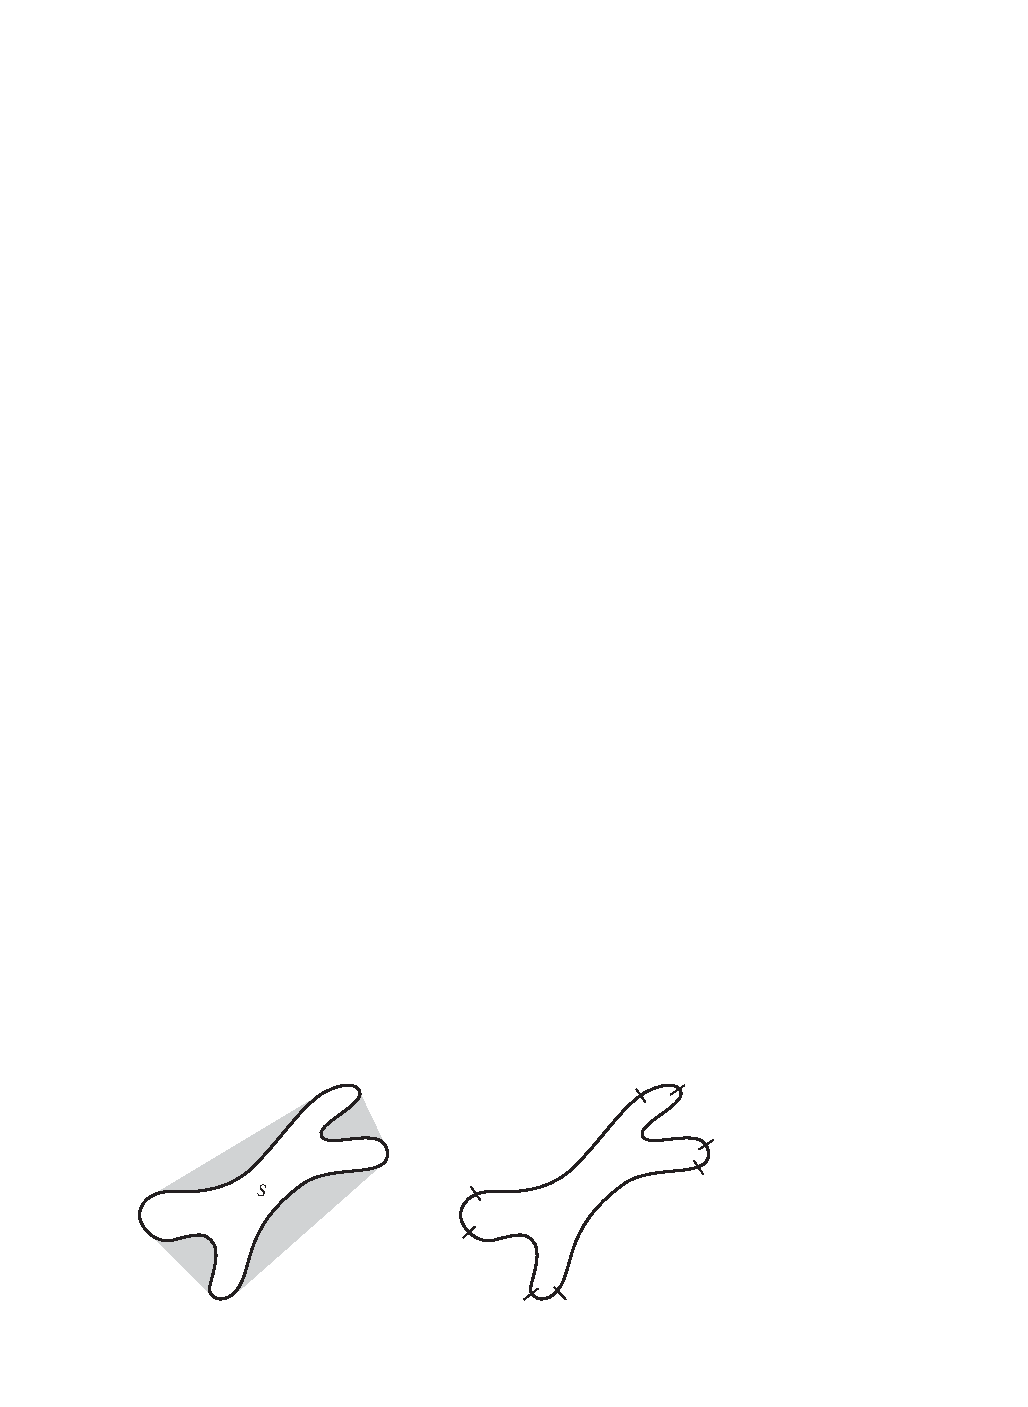
\includegraphics[scale=0.7]{Feature12}
\caption{(a) A region, $S$, and its convex deficiency (shaded). (b) Partitioned boundary.}
\end{figure}
\end{frame}

\begin{frame}{Skeletonization}
\begin{itemize}
\item One way to represent a shape is to reduce it to a graph, by obtaining its \textit{\color{mycolor1}skeleton} via thinning (\textit{\color{mycolor1}skeletonization})
\item \textit{\color{mycolor2}MAT (Medial axis transformation)} is composed by all the points which have more than one 
closest boundary points (``\textit{\color{mycolor2}prairie fire concept}'')
\end{itemize}
\begin{figure}
\subfigure[]{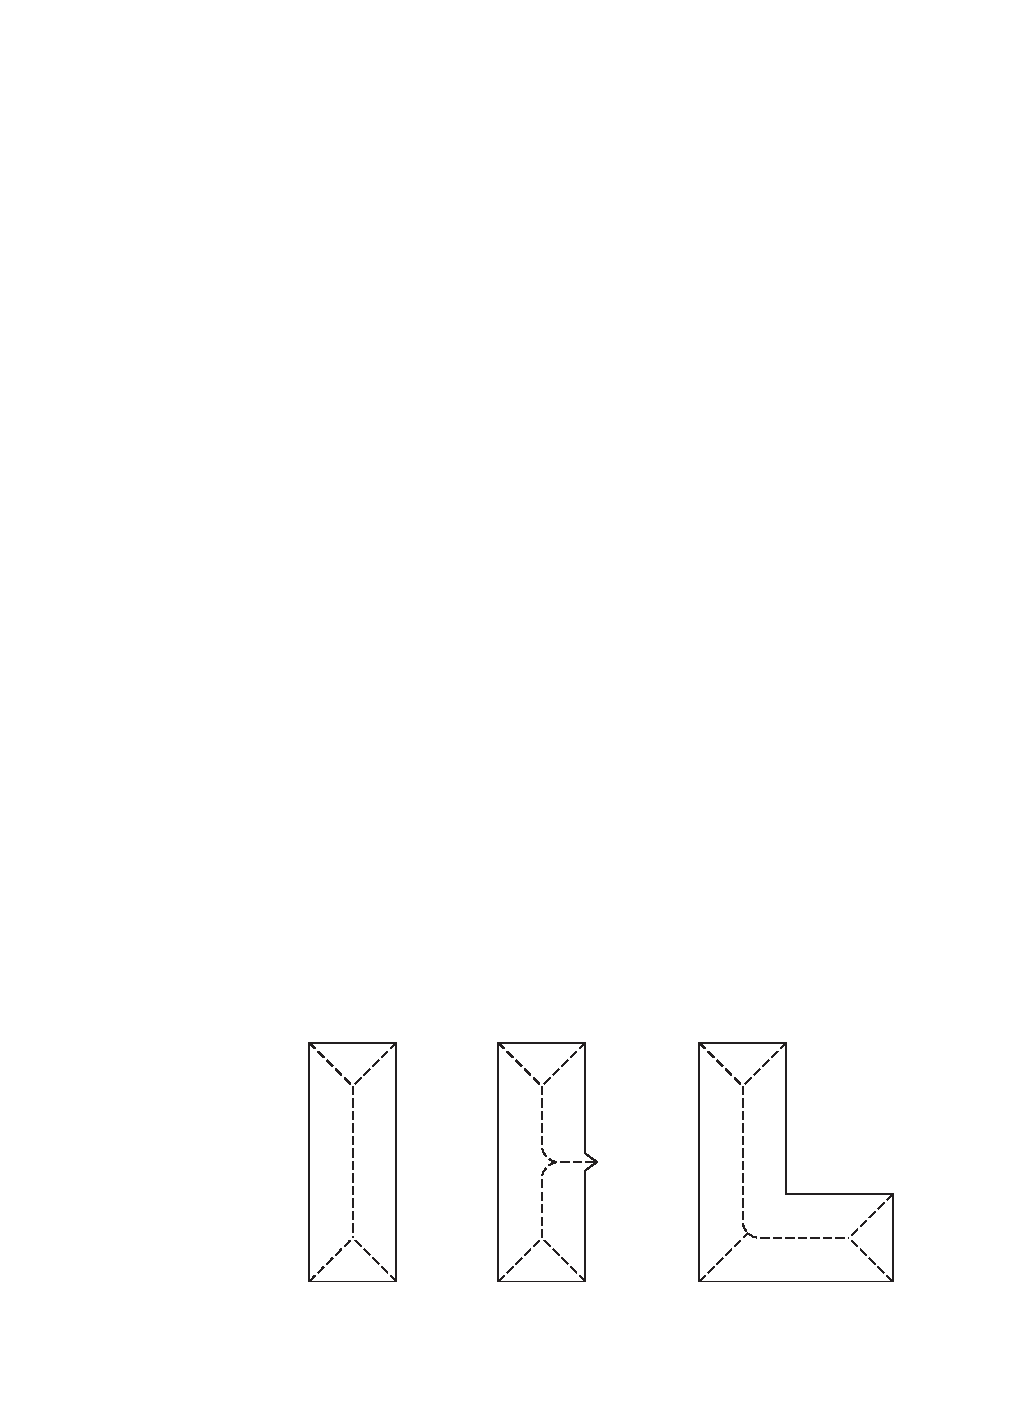
\includegraphics[scale=0.6]{Feature13}}~~~
\subfigure[]{
\includegraphics[scale=0.4]{Feature14}}
\caption{(a) Medial axes (dashed) of three simple regions,(b) Human leg bone and skeleton of the region}
\end{figure}
\end{frame}

\section{Boundary Descriptors}
\subsection{}

\begin{frame}{}
\begin{variableblock}{\centering \Large \textbf{\vspace{4pt}\newline Boundary Features/Descriptors\vspace{4pt}}}{bg=slidecolor,fg=white}{bg=slidecolor,fg=white}
\end{variableblock}
\end{frame}

\begin{frame}{Simple descriptors}
\vspace{-4pt}
\begin{itemize}
\item \textit{\color{mycolor1}length} of a boundary is one of its simplest descriptors.
\begin{itemize}
\item The number of pixels along a boundary gives a rough approximation of its length.
\item For a chain coded curve with unit spacing:
\[\boxed{\textit{\color{mycolor1}length} ={\rm Horizontal}+{\rm Vertical}+\sqrt{2}\times {\rm Diagonal}}\]
\end{itemize}
%where, Horizontal is the no. horizontal components, Vertical is the no. of vertical components, and Diagonal is the no. of diagonal components.
\item \textit{\color{mycolor1}diameter} (length of the major axis)
\[\boxed{{\rm Diam}(B)=\max_{i,j}{[D(p_i,p_j)]}}\]
\item The \textit{\color{mycolor1}minor axis} of a boundary is defined as the 
line perpendicular to the \textit{\color{mycolor1}major axis}.
\item \textit{\color{mycolor1}Basic rectangle} (formed by the major and the minor axis; 
encloses the boundary) and its
\[\boxed{{\sf \color{mycolor2} eccentricity}=\frac{\it \sf major~axis}{\it \sf minor~axis}}\]
\end{itemize}
\end{frame}

\begin{frame}{Shape Number}
\begin{itemize}
\item {\color{mycolor1}Shape number:} the first difference as {\color{mycolor2}smallest magnitude} (treating the chain code as a circular sequence)
\item {\color{mycolor1}Order of a shape:} the number of digits in Shape number.
\end{itemize}
\vspace{-0.5cm}
\begin{figure}
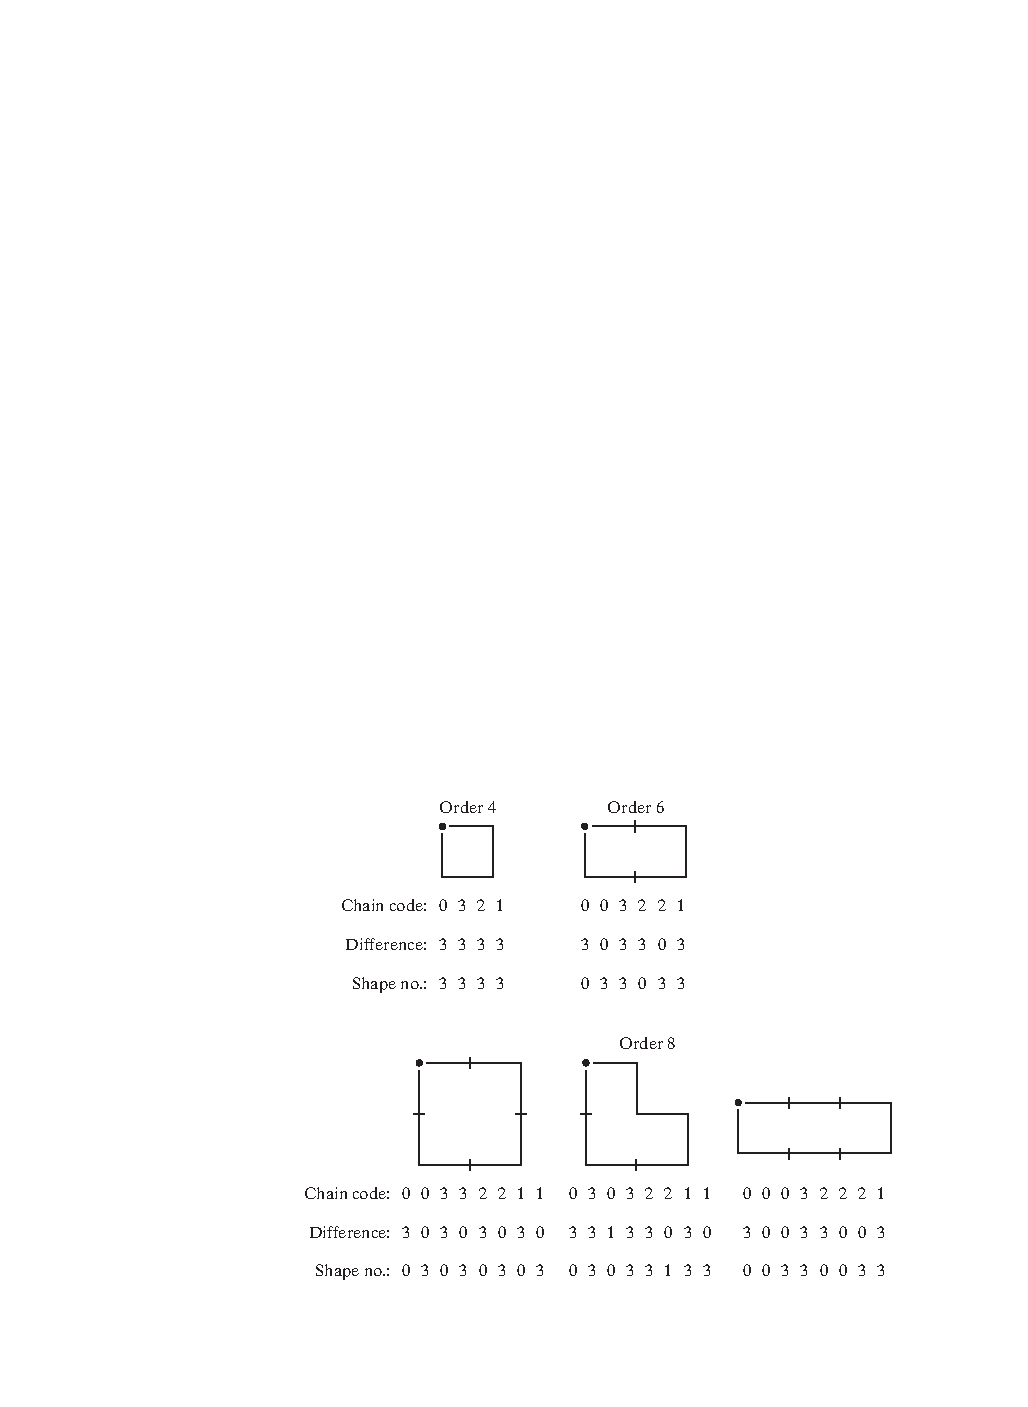
\includegraphics[scale=0.64]{Feature04}~~~
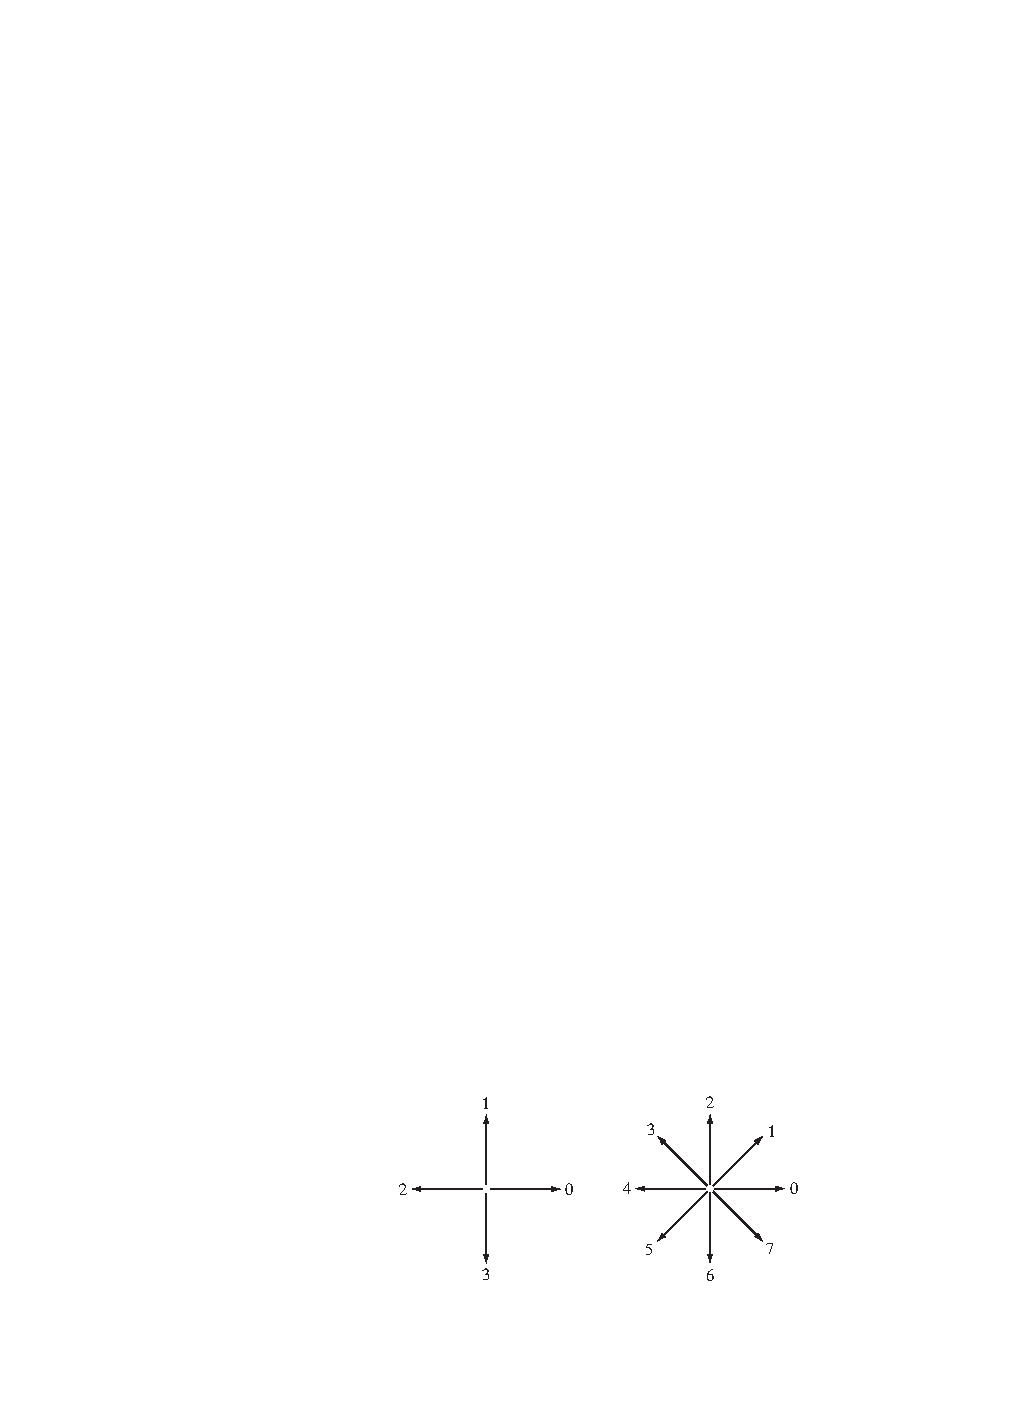
\includegraphics[scale=0.64]{Feature01}
\end{figure}
\end{frame}

\begin{frame}{Shape Number}
\begin{itemize}
\item It is advisable to normalize the grid orientation by {\color{mycolor4}aligning} the chain code grid {\color{mycolor4}to the basic rectangle}.
\end{itemize}
\begin{figure}
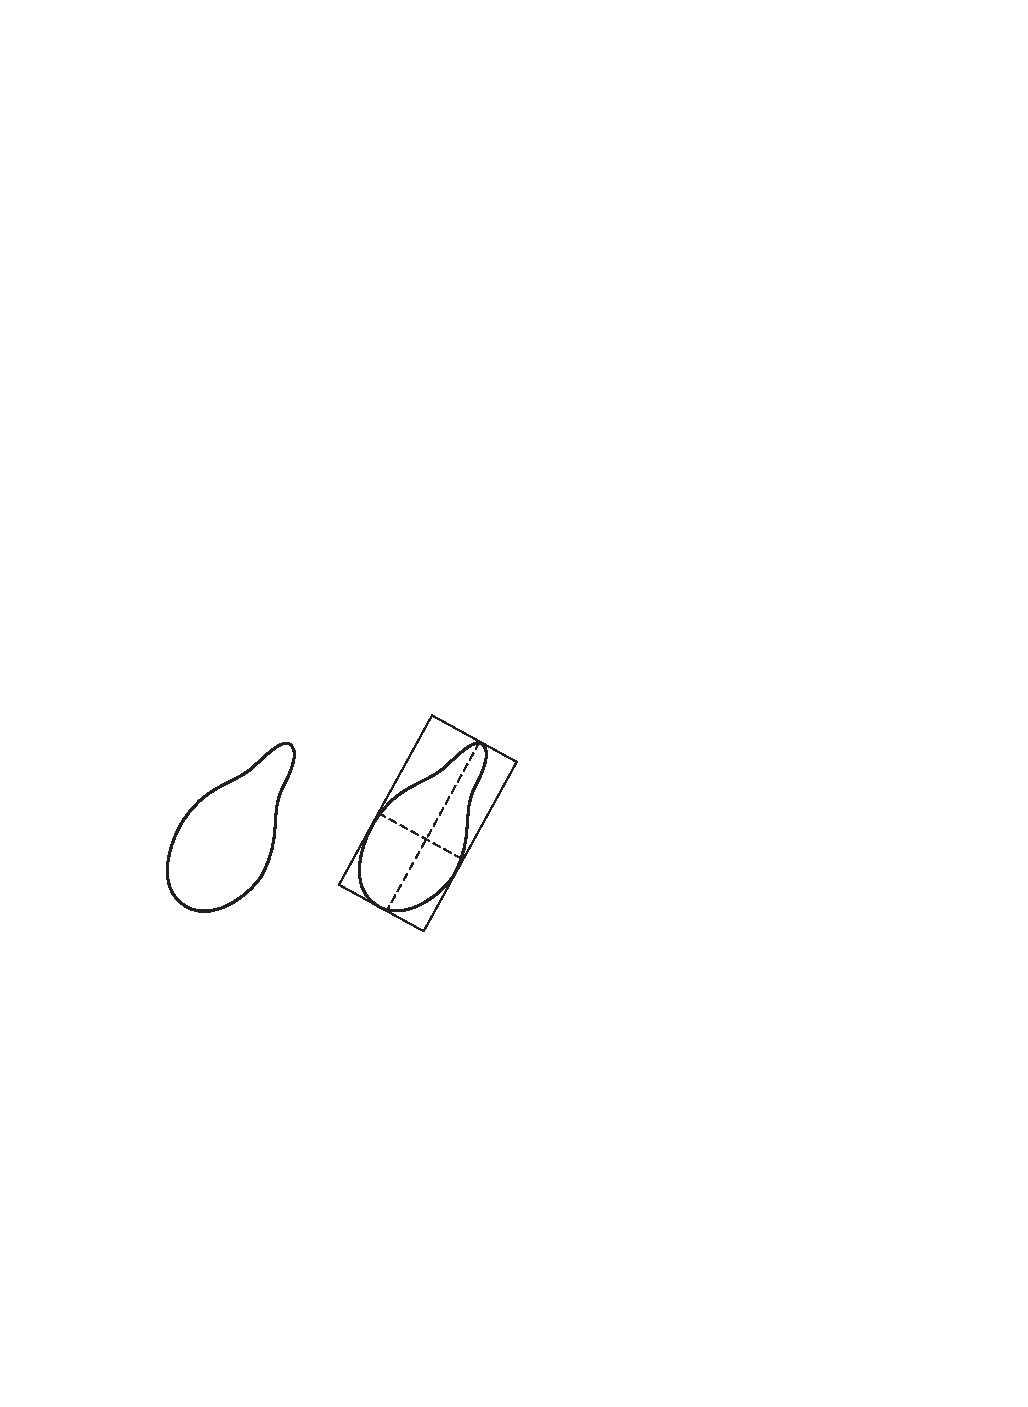
\includegraphics[scale=0.7]{Figures/Feature05}~~
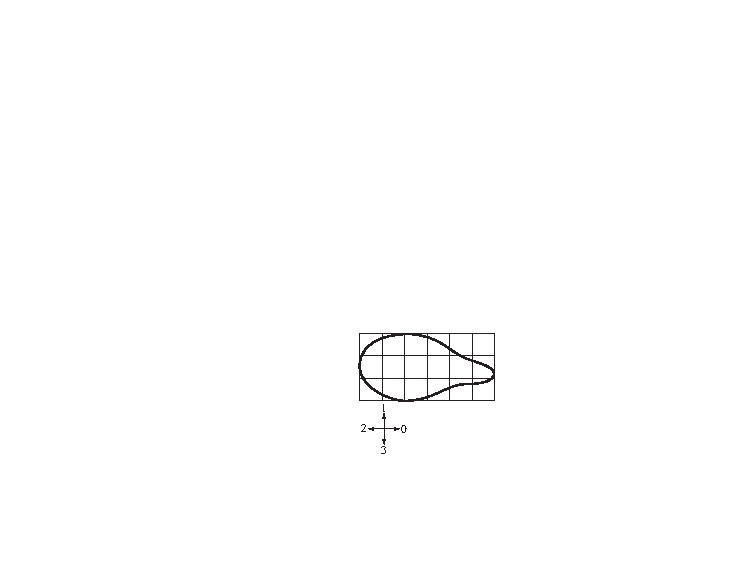
\includegraphics[scale=1]{Figures/Feature05e}~~
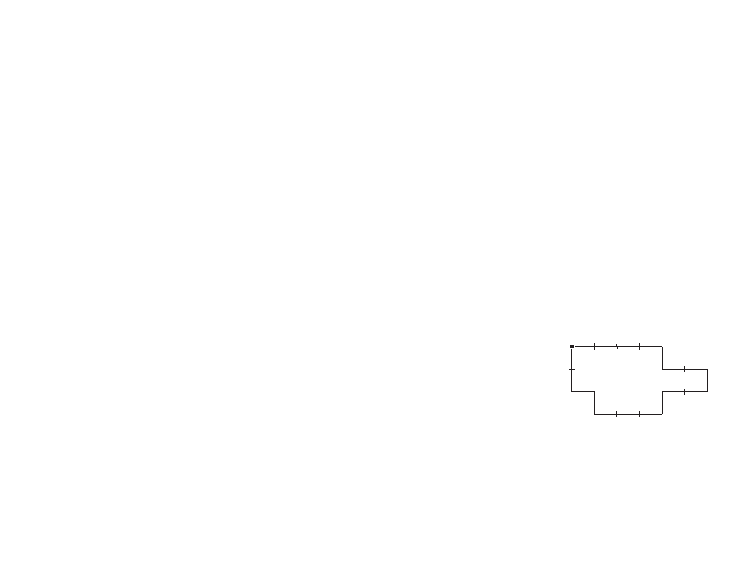
\includegraphics[scale=1]{Figures/Feature05f}
\end{figure}
\begin{figure}
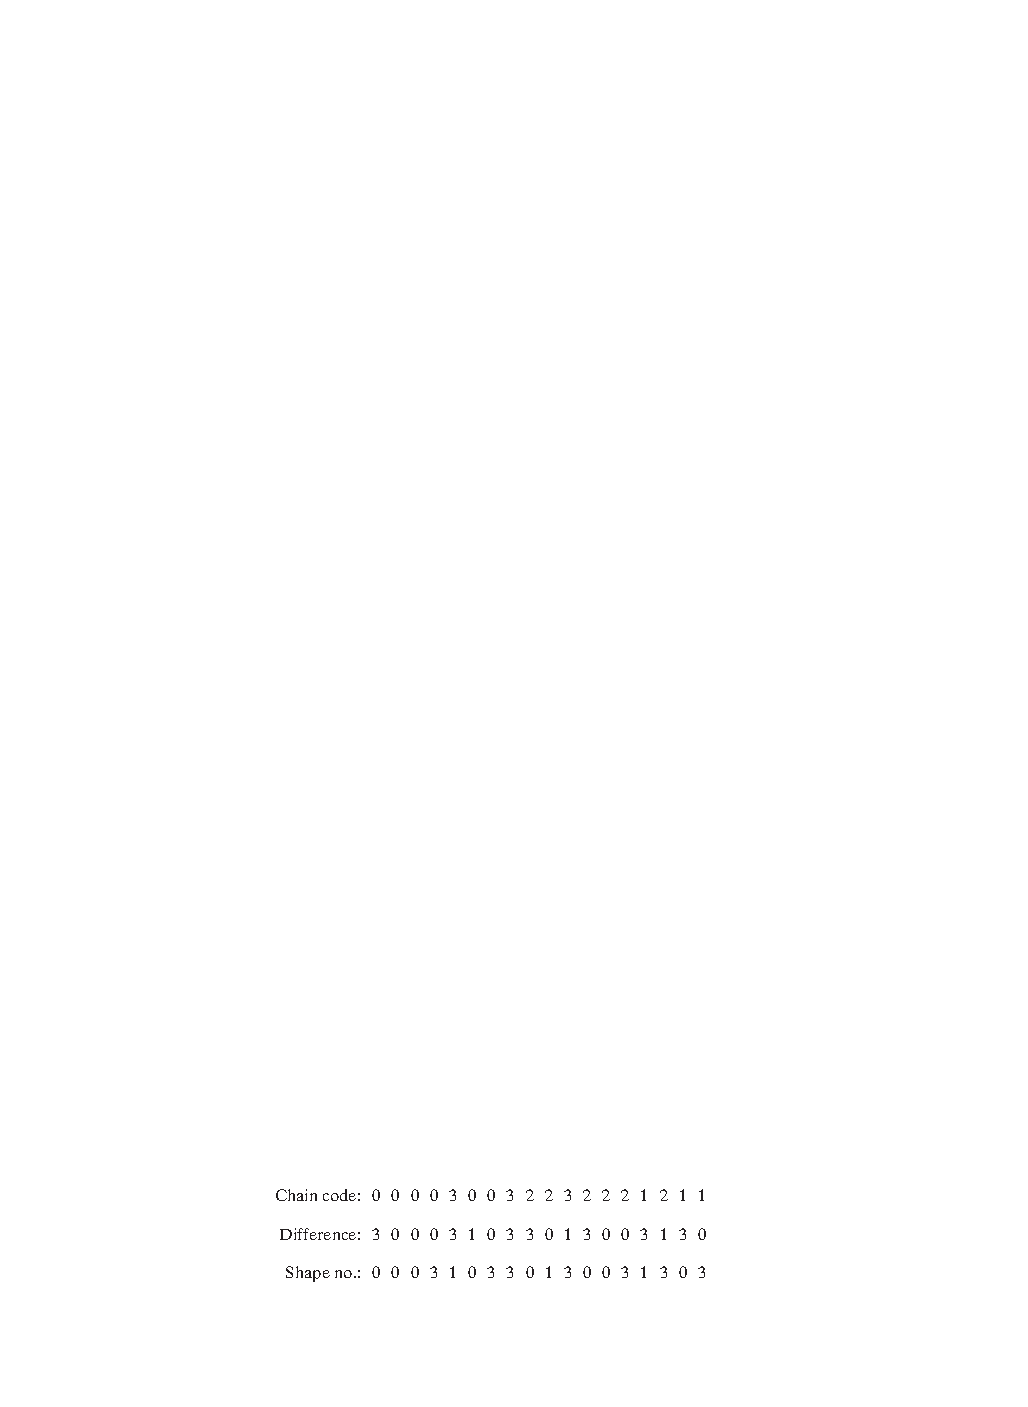
\includegraphics[scale=1]{Feature05a}
\end{figure}
\end{frame}

\begin{frame}{Fourier Descriptors}
\begin{figure}
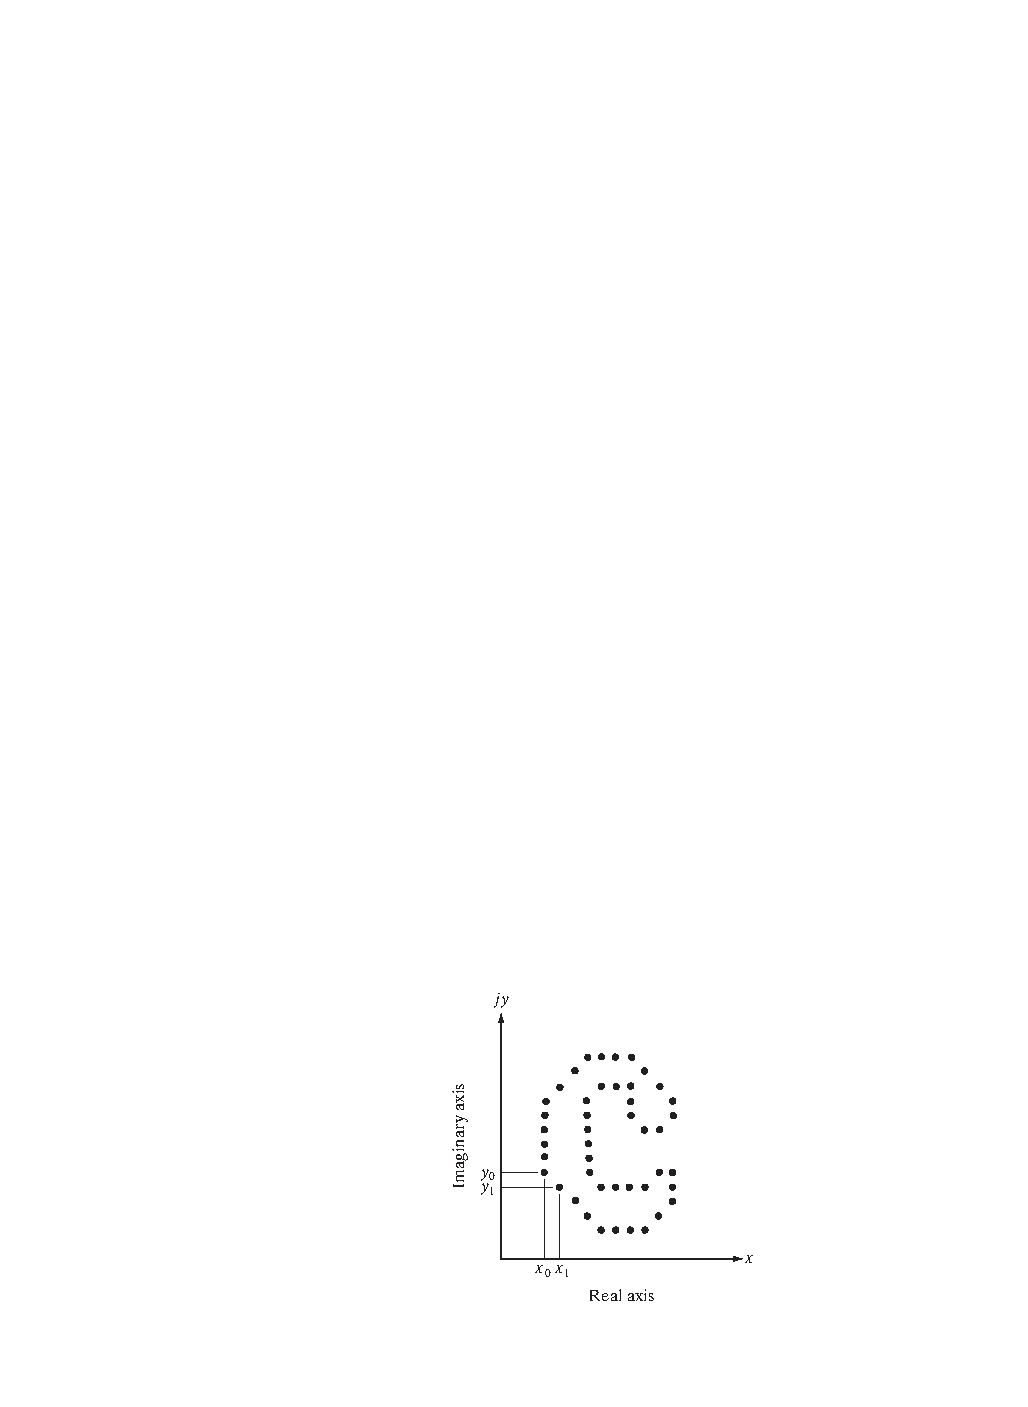
\includegraphics[scale=1]{Feature30}
\caption{A digital boundary and its representation as a complex sequence. The point $(x_0,y_0)$ and $(x_1,y_1)$ shown are (arbitrarily) the first two points in the sequence.}
\end{figure}
\end{frame}

\begin{frame}{Fourier Descriptors}
\begin{itemize}
\item Each coordinate pair treat as a complex number
\[\boxed{s(k)=x(k)+jy(k)}\]
for $k=0,1,2,\ldots, N-1$.
\item The discrete Fourier transform (DFT) of $s(k)$ is
\[\boxed{a(u) = \sum\limits_{k = 0}^{N - 1} {s(k){e^{ - j2\pi uk/N}}} }\]
for $u=0,1,2,\ldots,N-1$
\item $a(u)$ are Fourier Descriptors.
\end{itemize}
\end{frame}

\begin{frame}{Statistical moments}
\vspace{-4pt}
\begin{figure}
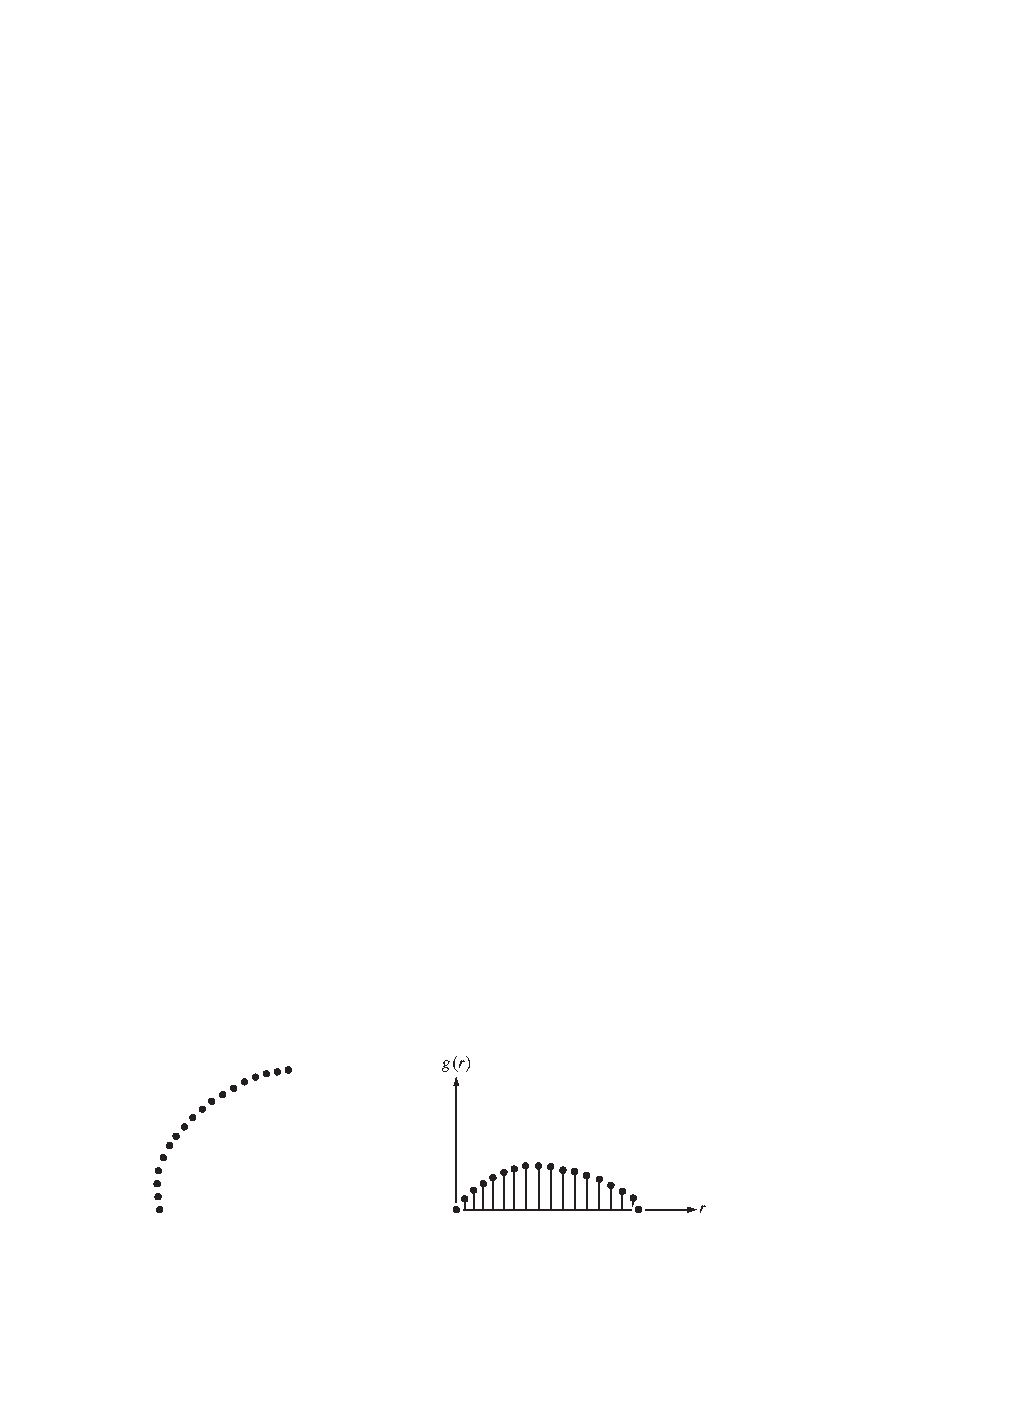
\includegraphics[scale=0.7]{Feature27}
\end{figure}
\begin{itemize}
\item Once a boundary is described as a 1-D function, {\color{mycolor2}statistical moments} (mean, variance, and a few higher-order central moments) can be used to describe it.
\[\boxed{{\mu _n}(z) = \sum\limits_{i = 0}^{N - 1} {{{({z_i} - m)}^n}p({z_i})}} \]
\[\boxed{m = \sum\limits_{i = 0}^{N - 1} {{z_i}p({z_i})}} \]

%\begin{figure}
%\includegraphics[scale=1]{Feature28}\\
%\includegraphics[scale=1]{Feature29}
%\end{figure}
\end{itemize}
\end{frame}

\section{Regional Descriptors}
\subsection{}

\begin{frame}{}
\begin{variableblock}{\centering \Large \textbf{\vspace{4pt}\newline Regional Features/Descriptors\vspace{4pt}}}{bg=slidecolor,fg=white}{bg=slidecolor,fg=white}
\end{variableblock}
\begin{figure}
\centering
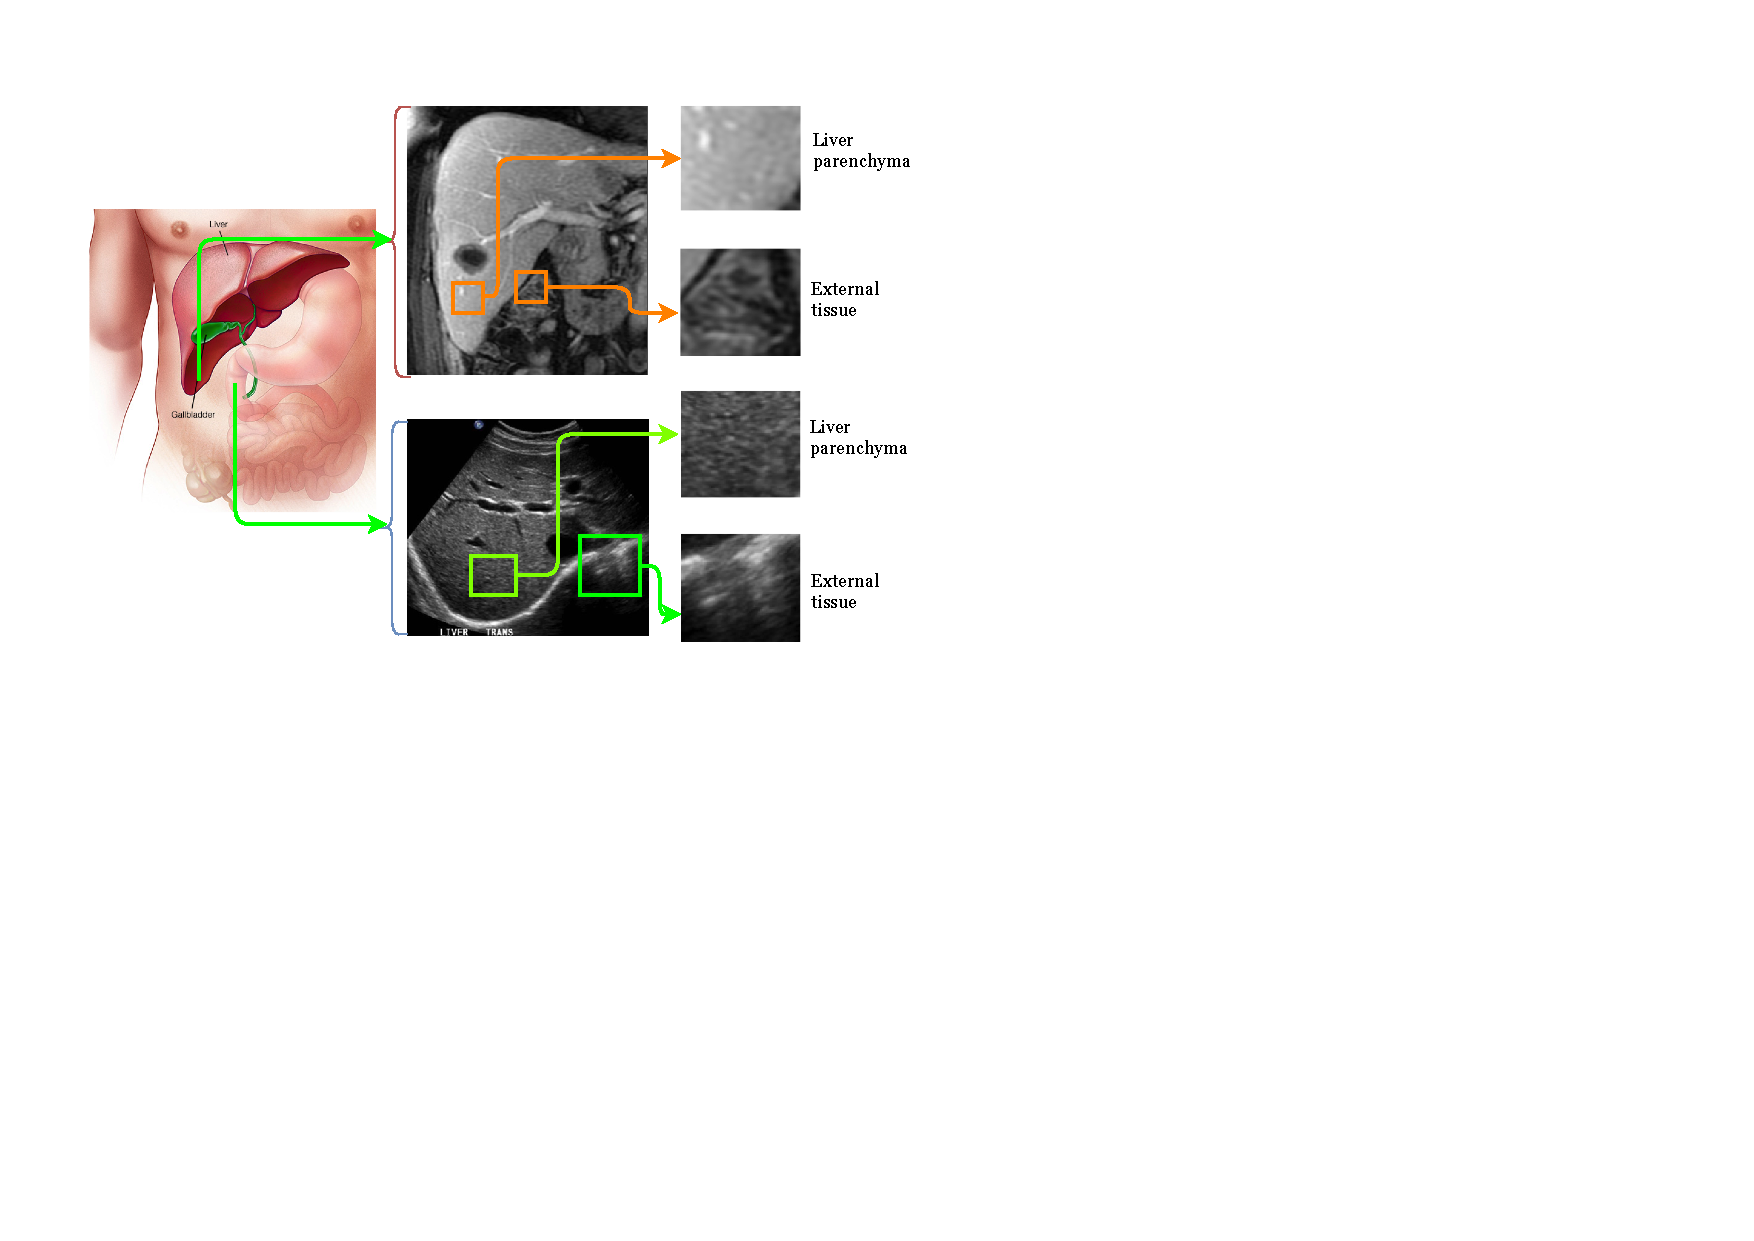
\includegraphics[scale=0.6]{Figures/FE008}
\end{figure}
\end{frame}

\begin{frame}{Some simple Descriptors}
\begin{itemize}
\item The \textit{\color{mycolor1}area of a region} is defined as the number of 
pixels in the region.
\item The \textit{\color{mycolor1}perimeter of a region} is the length of its 
boundary.
\item \textit{\color{mycolor1}Compactness of a region}, defined as 
$(perimeter)^2/area$, and is minimal for a disk-shape 
region.
\item A slightly different descriptor of compactness is the \textit{\color{mycolor1}circularity ratio}, defined as the ratio of the area of a region to the area of a circle (the most compact shape).
\item \textit{\color{mycolor1}Region descriptors}:
\begin{itemize}
\item mean and median of the gray levels,
\item minimum and maximum gray-level values, and
\item number of pixels with above and below the mean.
\end{itemize}
\end{itemize}
\end{frame}

\begin{frame}{Region Features}
\begin{itemize}
\setlength{\itemsep}{12pt}
\item There are following region features
\begin{itemize}
\item Colors, e.g., RGB values, HSV value, L*a*b
\item Intensity, e.g. Gray Values
\item Textures
\end{itemize}
\item Further texture is divided into two classes:
\begin{itemize}
\item Spatial Domain Features
\begin{itemize}
\item Structural Features, e.g., LBP, Wavelets
\item Statistical Features, e.g., GLCM, Orientation Histogram
\end{itemize}
\item Transformed Domain Features
\begin{itemize}
\item Gabor Filters
\end{itemize}
\end{itemize}
\end{itemize}
\end{frame}

\begin{frame}{Texture}
\begin{itemize}
\item An important approach to region description is 
to quantify its texture content.
\begin{figure}
\includegraphics[scale=0.65]{Feature15}
\caption{The white squares mark, from left to
right, smooth, coarse, and regular textures. These are optical microscope images of a superconductor, human cholesterol, and a
microprocessor. (Courtesy of Dr. Michael W.
Davidson, Florida State University.)}
\end{figure}
\end{itemize}
\end{frame}

\begin{frame}{Texture: Statistical approaches}
\begin{itemize}
\item Compute the \textit{\color{mycolor1}histogram} of the \textit{\color{mycolor1}area of interest}.
\item The \textit{\color{mycolor1}$n^{th}$ moment} of $z$ about the mean is
\[\boxed{{\mu _n}(z) = \sum\limits_{i = 0}^{L - 1} {{{({z_i} - m)}^n}p({z_i})}}~~~~~~~\boxed{m = \sum\limits_{i = 0}^{L - 1} {{z_i}p({z_i})}}  \]
\item The \textit{\color{mycolor1}second moment} ($n=2$) is of particular importance in 
texture description. It is a measure of gray-level contrast that can be used 
to establish descriptors of relative \textit{\color{mycolor1}smoothness}.
\item  For example, the texture measure, $R$, is 0 for areas of contrast intensity (the variance is 0 here) and approaches 1 for 
large value of $\sigma^2(z)$
\[\boxed{R=1-\frac{1}{1+\sigma^2(z)}}\]
\end{itemize}
\end{frame}

\begin{frame}{Texture: Statistical approaches}
\vspace{-8pt}
\begin{small}
\begin{itemize}
\item The \textit{\color{mycolor1}third moment} 
\[\boxed{{\mu _3}(z) = \sum\limits_{i = 0}^{L - 1} {{{({z_i} - m)}^3}p({z_i})}} \]
%\begin{figure}
%\includegraphics[scale=1]{Feature18}
%\end{figure}
is a measure of the \textit{\color{mycolor1}skewness} of the histogram while the \textit{\color{mycolor1}fourth moment} is a measure of its relatives flatness.
\item Some useful additional texture measures bases on histograms include a measure of ``\textit{\color{mycolor1}uniformity}'', given by
\[\boxed{{\rm Uniformity} = \sum\limits_{i = 0}^{L - 1} {{p^2}({z_i})} }\]
%\begin{figure}
%\includegraphics[scale=1]{Feature19}
%\end{figure}
\item \textit{\color{mycolor1}Average entropy} measure
\[\boxed{{\rm Entropy} =  - \sum\limits_{i = 0}^{L - 1} {p({z_i}){{\log }_2}p({z_i})} }\]
%\begin{figure}
%\includegraphics[scale=1]{Feature20}
%\end{figure}
\end{itemize}
\end{small}
\end{frame}

\begin{frame}{Texture: Statistical approaches}
\begin{figure}
\caption{Texture measures for the subimages shown in previous slide}
\includegraphics[scale=0.9]{Feature25}
\end{figure}
\end{frame}

\begin{frame}{Image Histograms}
\begin{itemize}
\item The {\color{mycolor2}histogram} of a digital image with intensity levels in the range $[0,L-1]$ is a discrete function
\begin{equation}
h(r_k) = n_k
\end{equation}
where, $r_k$ is the $k$th intensity value and $n_k$ is the number of pixels in the image with intensity $r_k$
\item Normalized histogram
\begin{equation}
p(r_k) = \frac{r_k}{MN}~~~~~\text{for}~k=0,1,2,\ldots,L-1.
\end{equation}
\item $p(r_k)$ is an estimate of the probability of occurrence of intensity level $r_k$ in an image.
\end{itemize}
\end{frame}

\begin{frame}{Compute histogram}
Compute the histogram of the given image. First find out the number graylevels in the image (how many bit image?).
\begin{figure}
\onslide<1->{\includegraphics[height=3.5cm]{Hist03}~~~}
\onslide<2->{\includegraphics[height=3.5cm]{aa}}
\end{figure}
\end{frame}

\begin{frame}{Texture: Gray level co-occurrence matrix (GLCM)}
\begin{itemize}
\begin{small}
\item Gray Level Co-occurance Matrix:  $G_{l,\theta}(i,j)$\\
where $i=0,1,2,\ldots,L-1$, $j=0,1,2,\ldots,L-1$, $L$ is maximum intensity level.
\begin{figure}
\includegraphics[scale=0.85]{Feature21}
\end{figure}
\item Above calculation is just for demonstration. For real images, GLCM matrix dimension is $L\times L$, where index varies as $i=0,1,2,\ldots,L-1$, $j=0,1,2,\ldots,L-1$.
\end{small}
\end{itemize}
\end{frame}

\begin{frame}{GLCM Features}
\begin{footnotesize}
\begin{itemize}
\item \textit{\color{mycolor1}Maximum probability}: Measure of the strongest response of $G$. The range of value is $[0,1]$.
\begin{equation}
\boxed{\text{Maximum probability}=\max_{i,j}{p_{ij}}}\nonumber
\end{equation}
\item \textit{\color{mycolor1}Contrast}: A measure of intensity contrast between a pixel and its neighbor over the entire image. The range of values is 0 (When G is constant) to $(L-1)^2$.
%\begin{equation}
%\sum\limits_{i = 0}^{L-1} {\sum\limits_{j = 0}^{L-1} {{{(i - j)}^k}{p_{ij}}} }\nonumber
%\end{equation}
%for $k=2$, measure give the \textit{\color{mycolor1} contrast} of that region.
\begin{equation}
\boxed{{\rm Contrast} = \sum\limits_{i = 0}^{L-1} {\sum\limits_{j = 0}^{L-1} {{{(i - j)}^2}{p_{ij}}} }}\nonumber
\end{equation}
\item \textit{\color{mycolor1}Inverse Element Difference Moment}: A measure of intensity contrast between a pixel and its neighbor.
\begin{equation}
\sum\limits_{i = 0}^{L-1} {\sum\limits_{j = 0}^{L-1} {\frac{{{p_{ij}}}}{{{{(i - j)}^k}}}} } ~~~~~~{\text{for}~ i\neq j}\nonumber
\end{equation}
\end{itemize}
\end{footnotesize}
\end{frame}

\begin{frame}{GLCM Features}
\begin{footnotesize}
\begin{itemize}

\item \textit{\color{mycolor1}Uniformity/Energy}: A measure of how intensities are uniformly distributed.
\begin{equation}
\boxed{{\rm Uniformity} = \sum\limits_{i = 0}^{L-1} {\sum\limits_{j = 0}^{L-1} {{p_{ij}}^2} }} \nonumber
\end{equation}
\item \textit{\color{mycolor1}Homogeneity}: Measures the spatial closeness of the distribution of elements in $G$ to the diagonal. The range of values is [0,1], with the maximum being achieved when $G$ is a diagonal matrix.
\begin{equation}
\boxed{{\rm Homogeneity} = \sum\limits_{i = 0}^{L-1} {\sum\limits_{j = 0}^{L-1} {\frac{{{p_{ij}}}}{{1 + \left| {i - j} \right|}}} }}\nonumber
\end{equation}
also defined as
\begin{equation}
\boxed{{\rm Homogeneity} = \sum\limits_{i = 0}^{L-1} {\sum\limits_{j = 0}^{L-1} {\frac{{{p_{ij}}}}{{1 + \left( {i - j} \right)^2}}} }}\nonumber
\end{equation}
\end{itemize}
\end{footnotesize}
\end{frame}


\begin{frame}{GLCM Features}
\begin{footnotesize}
\begin{itemize}
\item \textit{\color{mycolor1}Entropy}: Measures the randomness of the elements of $G$. The entropy is 0 when all $p_{ij}$'s are 0 and is maximum when all $p_{ij}$'s are equal. The maximum value is $2\log_2{L}$.
\begin{equation}
\boxed{{\rm Entropy} = - \sum\limits_{i = 0}^{L-1} {\sum\limits_{j = 0}^{L-1} {{p_{ij}}{{\log }_2}} } {p_{ij}}}\nonumber
\end{equation}
\item \textit{\color{mycolor1}Correlation}: A measure of how correlated a pixel is to its neighbor over the entire image. Range of values is 1 to $-1$.
\begin{equation}
\boxed{{\rm Correlation} = \sum\limits_{i = 0}^{L-1} {\sum\limits_{j = 0}^{L-1} {\frac{(i-m_r)(j-m_c)p_{ij}}{\sigma_r \sigma_c}} }} \nonumber
\end{equation}
\[m_r = \sum\limits_{i = 0}^{L-1} i{\sum\limits_{j = 0}^{L-1} {{p_{ij}}} }~~~~~m_r = \sum\limits_{j = 0}^{L-1} j{\sum\limits_{i = 0}^{L-1} {{p_{ij}}} }\]
\[\sigma^2_r = \sum\limits_{i = 0}^{L-1} (i-m_r)^2{\sum\limits_{j = 0}^{L-1} {{p_{ij}}} }~~~~~\sigma^2_c = \sum\limits_{j = 0}^{L-1} (j-m_c)^2{\sum\limits_{i = 0}^{L-1} {{p_{ij}}} }\]
\end{itemize}
\end{footnotesize}
\end{frame}

\begin{frame}{GLCM feature Visualization}
\begin{figure}
\includegraphics[scale=0.45]{Figures/glcmImg01.pdf}\\
~~\includegraphics[scale=0.45]{Figures/glcmImg02.pdf}
\end{figure}
\end{frame}

\begin{frame}{Local Binary Pattern}
\vspace{-6pt}
\begin{small}
\begin{itemize}
\item Basic Local Binary Pattern is governed by
\[\boxed{{b_k} = \left\{ {\begin{array}{*{20}{c}}
  1&{\text{if~~}{g_k} \geqslant g(x)} \\ 
  0&\text{otherwise} 
\end{array}} \right.}\text{~~~~~and~~~~~}\boxed{LB{P_{ri}}(x) = \min \left\{ {{P_j}} \right\}}\]
where $P_j$ is decimal equivalent of binary sequence $b_j$.
\end{itemize}
\end{small}
\vspace{-6pt}
\begin{figure}
\centering
\includegraphics[width=0.8\textwidth]{Figures/FE010}
\end{figure}
\end{frame}

\begin{frame}{Local Binary Pattern: Example}
\begin{figure}
\centering
\includegraphics[width=.8\textwidth]{Figures/LBP001}
\end{figure}
\begin{tikzpicture}[remember picture,overlay]
  \pause
  \node (img1) at (2.1,2.8) {?};
    \node (img1) at (4.5,0.3) {Can you compute LBP at the position (?)?};
\end{tikzpicture}
\end{frame}

\begin{frame}{Local Binary Pattern: Example}
\begin{figure}
\centering
\includegraphics[width=0.7\textwidth]{Figures/LBP003.png}\\\vspace{0.2cm}
\includegraphics[width=0.2\textwidth]{Figures/tonyStark.jpg}~~~~
\includegraphics[width=0.2\textwidth]{Figures/TonyStarkGray.jpg}~~~~
\includegraphics[width=0.2\textwidth]{Figures/TonyStarkLBP.jpg}\\
\includegraphics[width=0.4\textwidth]{Figures/tonyStarkBar}
\end{figure}
\end{frame}

\section[TD Features]{Transformed Domain Features}
\subsection{}

\begin{frame}{}
\begin{variableblock}{\centering \Large \textbf{\vspace{4pt}\newline Transformed Domain Features\vspace{4pt}}}{bg=slidecolor,fg=white}{bg=slidecolor,fg=white}
\end{variableblock}
\end{frame}

%\begin{frame}{Transformed Domain Features}
%\begin{itemize}
%\item \textit{\color{mycolor1}Gabor Filters/Transform}
%\begin{figure}
%\includegraphics[scale=0.75]{Feature24}
%\end{figure}
%\end{itemize}
%\end{frame}

\begin{frame}{2D-Gabor filters}
\begin{itemize}
\item Gabor filters are bandpass filters which are used in image processing for
\begin{itemize}
\item feature extraction,
\item texture analysis, etc.
\end{itemize}   
\item In the spatial domain, a 2D Gabor filter is a Gaussian kernel function modulated by a sinusoidal wave. 
\begin{equation}
{g_{\lambda ,\theta ,\varphi ,\sigma ,\gamma }}(x,y) = \exp \left( { - \frac{{x{'^2} + {\gamma ^2}y{'^2}}}{{2{\sigma ^2}}}} \right)\exp \left( i\left({2\pi \frac{{x'}}{\lambda } + \varphi }\right) \right)\nonumber
\end{equation}
where $x'=x\cos\theta+y\sin \theta$ and $y'=-\sin \theta+y\cos \theta$.
\item It has been shown by several researchers that the profile of simple-cell receptive fields in the mammalian visual cortex can by described by oriented 2D-Gabor functions.
\end{itemize}
\end{frame}

\begin{frame}{2D-Gabor filters: Visual System}
\begin{itemize}
\item Simple cells respond to bars and gratings of given
orientation.
\end{itemize}
\begin{figure}
\includegraphics[scale=0.59]{Figures/visualSystem.png}
\end{figure}
\end{frame}

\begin{frame}{2D Gabor Functions}
\begin{itemize}
\item Complex
\begin{equation}
{g_{\lambda ,\theta ,\varphi ,\sigma ,\gamma }}(x,y) = \exp \left( { - \frac{{x{'^2} + {\gamma ^2}y{'^2}}}{{2{\sigma ^2}}}} \right)\exp \left( i\left({2\pi \frac{{x'}}{\lambda } + \varphi }\right) \right)\nonumber
\end{equation}
\item Real
\begin{equation}
{g_{\lambda ,\theta ,\varphi ,\sigma ,\gamma }}(x,y) = \exp \left( { - \frac{{x{'^2} + {\gamma ^2}y{'^2}}}{{2{\sigma ^2}}}} \right)\cos \left( {2\pi \frac{{x'}}{\lambda } + \varphi } \right)\nonumber
\end{equation}
\item Imaginary
\begin{equation}
{g_{\lambda ,\theta ,\varphi ,\sigma ,\gamma }}(x,y) = \exp \left( { - \frac{{x{'^2} + {\gamma ^2}y{'^2}}}{{2{\sigma ^2}}}} \right)\sin \left( {2\pi \frac{{x'}}{\lambda } + \varphi } \right)\nonumber
\end{equation}
where
\begin{align*}
x'=&x\cos \theta +y\sin \theta\\
y'=&-x\sin \theta +y\cos \theta\\
\end{align*}
\end{itemize}
\end{frame}
%\section{Filter Parameter}
%\subsection{}
\begin{frame}{2D Gabor function parameters}
\begin{equation}
{g_{\lambda ,\theta ,\varphi ,\sigma ,\gamma }}(x,y) = \exp \left( { - \frac{{x{'^2} + {\gamma ^2}y{'^2}}}{{2{\sigma ^2}}}} \right)\cos \left( {2\pi \frac{{x'}}{\lambda } + \varphi } \right)\nonumber
\end{equation}
where
\begin{align*}
x'=&x\cos \theta +y\sin \theta\\
y'=&-x\sin \theta +y\cos \theta\\
\end{align*}
$\lambda\rightarrow$ wavelength of the sinusoidal factor,\\
$\theta\rightarrow$ orientation of the normal to the parallel stripes of a Gabor function,\\
$\varphi\rightarrow$ phase offset,\\
$\sigma\rightarrow$ standard deviation of the Gaussian envelope,\\
$\gamma\rightarrow$ spatial aspect ratio, specifies the ellipticity of the support of the Gabor function.
\end{frame}

%\begin{frame}{Wavelength ($\lambda$)}
%\begin{itemize}
%\item Wavelength of the cosine factor of the Gabor filter kernel.
%\item Value is to be specified in number of pixels.
%\item Valid values are real numbers, $\lambda\geq 2$
%\item The value $\lambda=2$ should not be used in combination with phase offset $\phi = -90$ or $\phi=90$, because in these cases the Gabor function is sampled in its zero crossings.
%\item To avoid undesirable effect at the image borders, $\lambda$ value should be smaller than one fifth of the input size.
%\begin{figure}
%\includegraphics[scale=0.8]{Figures/Gabor03}
%\caption{Image size is $100\times 100$, $\lambda=5,10,15$ from left to right, other parameters $\theta = 0$, $\varphi = 0$, $\gamma=0.5$, $b = 1$}
%\end{figure}
%\end{itemize}
%\end{frame}
%
%\begin{frame}{Orientations ($\theta$)}
%\begin{itemize}
%\item This parameter specifies the orientation of the normal to the parallel stripes of a Gabor function.
%\item Value is to be specified in degrees.
%\item Valid values are real numbers between $0-360$.
%\begin{figure}
%\includegraphics[scale=1]{Figures/Gabor04}
%\caption{Image size is $100\times 100$, $\theta=0,45,90$ from left to right, other parameters $\lambda = 10$, $\varphi= 0$, $\gamma=0.5$, $b = 1$}
%\end{figure}
%\end{itemize}
%\end{frame}
%
%\begin{frame}{Phase offset ($\varphi$)}
%\begin{itemize}
%\item The phase offset $\varphi$ in the cosine factor of the Gabor function is specified in degree.
%\item Valid values are real number in between $-180$ and $180$.
%\item The values 0 and 180 corresponds to center-symmetric `center-on' and `center-off' function, respectively. While $-90$ and $90$ corresponds to anti-symmetric functions
%\begin{figure}
%\includegraphics[scale=0.8]{Figures/Gabor06}
%\caption{Image size is $100\times 100$, $\phi=0,~180,~-90,~and~90$ degrees from left to right, other parameters $\lambda = 10$, $\theta = 0$, $\gamma=0.5$, $b = 1$}
%\end{figure}
%\end{itemize}
%\end{frame}
%
%\begin{frame}{Aspect ratio ($\gamma$)}
%\begin{itemize}
%\item This is spatial aspect ratio which specifies the ellipticity of the support of the Gabor function.
%\item For $\gamma=1$, the support is circular.
%\item For $\gamma <1$ the support is elongated in orientation of the parallel stripes of the function
%\item Normal value is $\gamma=0.5$
%\begin{figure}
%\includegraphics[scale=1]{Figures/Gabor07}
%\caption{Image size is $100\times 100$, $\gamma=0.5~and~1$ degrees from left to right, other parameters $\lambda = 10$, $\theta = 0$, $\varphi=0$, $b = 1$}
%\end{figure}
%\end{itemize}
%\end{frame}
%
%\begin{frame}{Bandwidth ($b$)}
%\begin{itemize}
%\item The half-response spatial frequency bandwidth $b$ (in octaves)  of a Gabor filter is related to the ratio $\frac{\sigma}{\lambda}$.
%%, where $\sigma$ and $\lambda$  are the standard deviation of the Gaussian factor of the Gabor function and the preferred wavelength, respectively.
%\[b = {\log _2}\frac{{\frac{\sigma }{\lambda }\pi  + \sqrt {\frac{{\ln 2}}{2}} }}{{\frac{\sigma }{\lambda }\pi  - \sqrt {\frac{{\ln 2}}{2}} }},~~~\frac{\sigma }{\lambda } = \frac{1}{\pi }\sqrt {\frac{{\ln 2}}{2}}  \cdot \frac{{{2^b} + 1}}{{{2^b} - 1}}\]
%\item The value of $\sigma$ cannot be specified directly. It can only be changed through the bandwidth $b$.
%\item Must be a real positive number.
%\item The smaller the bandwidth, the larger $\sigma$,
%\end{itemize}
%\end{frame}
%
%\begin{frame}{Spatial frequency (${1}/{\lambda}$)}
%\begin{itemize}
%\item Preferred spatial frequency, ${1}/{\lambda}$, and size $\sigma$ are not fully independent. Values are related with a relation
%\begin{equation}
%\sigma = a\lambda \nonumber
%\end{equation}
%\item $a$ varies in between $0.03$ and $0.6$ for most cells.
%\item In many experiments, $a=0.56$ is used, i.e., $\sigma=0.56\lambda$.
%\begin{figure}
%\includegraphics[scale=0.8]{Figures/Gabor08}
%\caption{Image size is $100\times 100$, $b=0.5,~1$~and~$2$ from left to right, respectively. Other parameters $\lambda = 10$, $\theta = 0$, $\varphi=0$, $\gamma= 0.5$}.
%\end{figure}
%\end{itemize}
%\end{frame}

\begin{frame}{Feature Vector from spectral bands}
\begin{columns}
\begin{column}{3.5cm}
\begin{figure}
\includegraphics[scale=0.47]{Figures/FE011}
\end{figure}
\end{column}
\begin{column}{7cm}
\begin{figure}
\includegraphics[scale=0.23]{Texture01}\\
\includegraphics[scale=0.138]{Texture02}~~
\includegraphics[scale=0.138]{Texture03}~~
\includegraphics[scale=0.138]{Texture04}\\
\includegraphics[scale=0.138]{Texture05}~~
\includegraphics[scale=0.138]{Texture06}~~
\includegraphics[scale=0.138]{Texture07}
\end{figure}
\end{column}
\end{columns}

\end{frame}

\begin{frame}{Feature Vector from spectral bands}
\begin{figure}
\includegraphics[scale=1]{Feature26}
\end{figure}
\end{frame}


%\begin{frame}{Assignment}
%\textit{\color{mycolor1}Question 01}:
%\begin{itemize}
%\item[i.] What is the order of the shape number for figure shown?
%\item[ii.] Obtain the shape number.
%\begin{figure}
%\includegraphics[scale=0.8]{Question01}
%\end{figure}
%\end{itemize}
%\textit{\color{mycolor1}Question 02}: Draw the Medial axis of the following
%\begin{itemize}
%\item[i.] Circle
%\item[ii.] Square
%\item[iii.] Rectangle
%\item[iv.] Equilateral Triangle
%\end{itemize}
%\end{frame}
%
%\begin{frame}{Assignment}
%\textit{\color{mycolor1}Question 03}:
%\begin{itemize}
%\item[i.] Compute gray level co-occurance matrix $G_{1,45^o}$ for given image.
%\begin{figure}
%\includegraphics[scale=0.25]{GLCM01}
%\end{figure}
%\item[ii.] Compute probability density function of GLCM matrix.
%\item[iii.] Compute Maximum probability, Correlation, Contrast, Uniformity (Energy), Homogeneity, and Entropy features.
%\end{itemize}
%\end{frame}
%
%\begin{frame}{Assignment}
%\textit{\color{mycolor1}Question 04}: Consider a binary image of size pixels, with a vertical black band extending from columns 1 to 99 and a vertical white band extending from columns 100 to 200
%\begin{itemize}
%\item[i.] Obtain the co-occurrence matrix of this image using the position operator
%``one pixel to the right.''
%\item[ii.]Normalize this matrix so that its elements become probability estimates.
%\item[iii.] Maximum probability, Correlation, Contrast, Uniformity (Energy), Homogeneity, and Entropy features.
%\end{itemize}
%\end{frame}
%
%\begin{frame}{Assignment}
%\textit{\color{mycolor1}Question 05}: Draw the signature of the following shapes:
%\begin{itemize}
%\item[i.] Equilateral Triangle
%\item[ii.] Rectangle
%\item[iii.] Ellipse
%\end{itemize}
%\textit{\color{mycolor1}Question 06}:
%\begin{itemize}
%\item[i.] Show that the first difference of a chain code normalizes it to rotation
%\item[ii.] Compute the first difference of the code 0101030303323232212111
%\end{itemize}
%\end{frame}

\section{References}
\subsection{}
\begin{frame}[allowframebreaks]{References}
\linespread{1}
\footnotesize
\printbibliography[heading=none]
\end{frame}
{
\setbeamertemplate{logo}{}
\makeatletter
\setbeamertemplate{footline}{
        \leavevmode%
  
  % First line.
  \hbox{%
  \begin{beamercolorbox}[wd=.2\paperwidth,ht=\beamer@decolines@lineup,dp=0pt]{}%
  \end{beamercolorbox}%
  \begin{beamercolorbox}[wd=.8\paperwidth,ht=\beamer@decolines@lineup,dp=0pt]{lineup}%
  \end{beamercolorbox}%
  } %
  % Second line.
  \hbox{%
  \begin{beamercolorbox}[wd=\paperwidth,ht=\beamer@decolines@linemid,dp=0pt]{linemid}%
  \end{beamercolorbox}%
  } %
  % Third line.
  \hbox{%
  \begin{beamercolorbox}[wd=.1\paperwidth,ht=\beamer@decolines@linebottom,dp=0pt]{}%
  \end{beamercolorbox}%
  \begin{beamercolorbox}[wd=.9\paperwidth,ht=\beamer@decolines@linebottom,dp=0pt]{linebottom}%
  \end{beamercolorbox}%
  }%
        }
\makeatother

\begin{frame}
\centering
\includegraphics[width=0.4\paperwidth]{queries.jpg}\\
\includegraphics[width=0.5\paperwidth]{thank_you.png}
\end{frame}
}



